% !TEX TS-program = xelatex
% Command for running this example (needs latexmkrc file):
%    latexmk -bibtex -pdf main.tex

% این قالب با استفاده از کلاس kntu-thesis جهت نگارش گزارش پروژه، پایان‌نامه و رساله توسط محمدسینا اله‌کرم آماده سازی شده و از طریق لینک زیر در دسترس علاقه‌مندان قرار گرفته است.
%	https://github.com/msinamsina/kntu-thesis

%----------------------------------------------------------------------------------------------
% اگر قصد نوشتن پروژه کارشناسی را دارید، در خط زیر به جای msc، کلمه bsc و اگر قصد نوشتن رساله دکترا را دارید، کلمه phd را قرار دهید. کلیه تنظیمات لازم، به طور خودکار، اعمال می‌شود.

% اگر مایلید پایان‌نامه شما دورو باشد به جای oneside در خط زیر از twoside استفاده کنید.

% برای حاشیه‌نویسی و کم کردن صفحات ابتدایی، گزینه draft را وارد و برای نسخه نهایی آن را حذف کنید.

% برای استفاده از قلم‌های سری IR Series گزینه irfonts را وارد و برای استفاده از قلم‌های X Series 2 آن را حذف کنید.

\documentclass[
twoside
% ,openany
,msc
,irfonts
% ,draft
]{./kntu-thesis}

% فایل commands.tex را مطالعه کنید؛ چون دستورات مربوط به فراخوانی بسته‌ها، فونت و دستورات خاص در این فایل قرار دارد.
% در این فایل، دستورها و تنظیمات مورد نیاز، آورده شده است.
%-------------------------------------------------------------------------------------------------------------------
% دستوراتی که پوشه پیش‌فرض زیرفایل‌های tex را مشخص می‌کند.
%\makeatletter
%\def\input@path{{./tex/}}
%\makeatother
% در ورژن جدید زی‌پرشین برای تایپ متن‌های ریاضی، این سه بسته، حتماً باید فراخوانی شود
\usepackage{amsthm,amssymb,amsmath}
% بسته‌ای برای تنطیم حاشیه‌های بالا، پایین، چپ و راست صفحه
\usepackage[a4paper, top=40mm, bottom=40mm, outer=25mm, inner=35mm]{geometry}
% بسته‌‌ای برای ظاهر شدن شکل‌ها و تعیین آدرس تصاویر
\usepackage[final]{graphicx}
\graphicspath{{./img/}}



% بسته‌های مورد نیاز برای نوشتن کدها، رنگ‌آمیزی آنها و تعیین پوشهٔ کدها
%%man ezafe kardam
\usepackage{subfig}

\usepackage{diagbox}
\usepackage{multirow}
\usepackage{rotating}
\usepackage[final]{listings}
\usepackage[usenames,dvipsnames,svgnames,table]{xcolor}
\lstset{inputpath=./code/}
\usepackage[notransparent]{svg}
\usepackage[final]{pdfpages}
\usepackage{tabularray}
\usepackage{booktabs, makecell, multirow, tabularx}
% بسته‌ای برای رسم کادر
\usepackage{framed} 
% بسته‌‌ای برای چاپ شدن خودکار تعداد صفحات در صفحه «معرفی پایان‌نامه»
\usepackage{lastpage}
% بسته‌ٔ لازم برای: ۱. تغییر شماره‌گذاری صفحات پیوست. ۲. تصحیح باگ آدرس وب حاوی '%' در مراجع
\usepackage{etoolbox}

%%%%%%%%%%%%%%%%%%%%%%%%%%%%%%%%%%%%
%%% دستورات وابسته به استیل مراجع:
%% اگر از استیل‌های natbib (plainnat-fa، asa-fa، chicago-fa) استفاده می‌کنید، خط زیر را فعال و بعدی‌اش را غیرفعال کنید.
%\usepackage{natbib}
%\newcommand{\citelatin}[1]{\cite{#1}\LTRfootnote{\citeauthor*{#1}}}
%\newcommand{\citeplatin}[1]{\citep{#1}\LTRfootnote{\citeauthor*{#1}}}


%% اگر از سایر استیل‌ها استفاده می‌کنید، خط بالا را غیرفعال و خط‌های زیر را فعال کنید.
\let\citep\cite
\let\citelatin\cite
\let\citeplatin\cite
%%%%%%%%%%%%
%% بررسی حالت پیش نویس
\usepackage{ifdraft}
\ifdraft
{%
	% بسته‌ٔ ایجاد لینک‌های رنگی با امکان جهش
	\usepackage[unicode=true,pagebackref=true,
colorlinks,linkcolor=blue,citecolor=blue,final]{hyperref}
	%\usepackage{todonotes}
	\usepackage[firstpage]{draftwatermark}
	\SetWatermarkText{\ \ \ \rl{پیش‌نویس}}
	\SetWatermarkScale{1.2}
}
{ 
	\usepackage[pagebackref=false]{hyperref}
	%\usepackage[disable]{todonotes} % final without TODOs
}

\usepackage[obeyDraft]{todonotes}
\setlength{\marginparwidth}{2cm}

%%%%%%%%%%%%
%%% تصحیح باگ: اگر در مراجع، آدرس وب حاوی '%' بوده و pagebackref فعال باشد، دستورات زیر باید بیایند:
%% برای استیل‌های natbib مثل plainnat-fa، asa-fa، chicago-fa
\makeatletter
\let\ORIG@BR@@lbibitem\BR@@lbibitem
\apptocmd\ORIG@BR@@lbibitem{\endgroup}{}{}
\def\BR@@lbibitem{\begingroup\catcode`\%=12 \ORIG@BR@@lbibitem}
\makeatother
%% برای سایر استیل‌ها
\makeatletter
\let\ORIG@BR@@bibitem\BR@@bibitem
\apptocmd\ORIG@BR@@bibitem{\endgroup}{}{}
\def\BR@@bibitem{\begingroup\catcode`\%=12 \ORIG@BR@@bibitem}
\makeatother
%%%%%%%%%%%%%%%%%%%%%%%%%%%%%%%%%%%%

% بسته‌ لازم برای تنظیم سربرگ‌ها
\usepackage{fancyhdr}
%\usepackage{enumitem}
\usepackage{setspace}
% بسته‌های لازم برای نوشتن الگوریتم
\usepackage{algorithm}
\usepackage{algorithmic}
% بسته‌های لازم برای رسم بهتر جداول
\usepackage{tabulary}
\usepackage{tabularx}
\usepackage{rotating}
% بسته‌های لازم برای رسم تنظیم بهتر شکل‌ها و زیرشکل‌ها
\usepackage[export]{adjustbox}
\usepackage{subfig}
\usepackage[subfigure]{tocloft}
% بسته‌ای برای رسم نمودارها و نیز صفحه مالکیت اثر
\usepackage{tikz}
% بسته‌ای برای ظاهر شدن «مراجع» و «نمایه» در فهرست مطالب
\usepackage[nottoc]{tocbibind}
% دستورات مربوط به ایجاد نمایه
\usepackage{makeidx}
\makeindex


% بسته‌ای برای افزودن تورفتگی به ابتدای اولین پاراگراف هر بخش
\usepackage{indentfirst}

% بسته زیر باگ ناشی از فراخوانی بسته‌های زیاد را برطرف می‌کند.
\usepackage{morewrites}
%%%%%%%%%%%%%%%%%%%%%%%%%%
%khodam
\RequirePackage{zref-perpage}
\zmakeperpage{footnote}

%%% بسته ایجاد واژه‌نامه با xindy
\usepackage[xindy,toc,acronym,nonumberlist=true]{glossaries}

% فراخوانی بسته زی‌پرشین (باید آخرین بسته باشد)
\usepackage[extrafootnotefeatures, localise=on, displaymathdigits=persian]{xepersian}
\paragraphfootnotes

\makeatletter
% تعریف قلم فارسی و انگلیسی و مکان قلم‌ها
\if@irfonts
\settextfont[Path={./font/}, BoldFont={IRLotusICEE_Bold.ttf}, BoldItalicFont={IRLotusICEE_BoldIranic.ttf}, ItalicFont={IRLotusICEE_Iranic.ttf},Scale=1.2]{IRLotusICEE.ttf}
% LiberationSerif or FreeSerif as free equivalents of Times New Roman
\setlatintextfont[Path={./font/}, BoldFont={LiberationSerif-Bold.ttf}, BoldItalicFont={LiberationSerif-BoldItalic.ttf}, ItalicFont={LiberationSerif-Italic.ttf},Scale=1]{LiberationSerif-Regular.ttf}
% چنانچه می‌خواهید اعداد در فرمول‌ها، انگلیسی باشد، خط زیر را غیرفعال کنید
% و گزینهٔ displaymathdigits=persian را از خط ۱۰۹ حذف کنید.
\setdigitfont[Path={./font/}, Scale=1.2]{IRLotusICEE.ttf}
% تعریف قلم‌های فارسی و انگلیسی اضافی برای استفاده در بعضی از قسمت‌های متن
\setiranicfont[Path={./font/}, Scale=1.3]{IRLotusICEE_Iranic.ttf}				% ایرانیک، خوابیده به چپ
\setmathsfdigitfont[Path={./font/}]{IRTitr.ttf}
\defpersianfont\titlefont[Path={./font/}, Scale=1]{IRTitr.ttf}
% برای تعریف یک قلم خاص عنوان لاتین، خط بعد را فعال و ویرایش کنید و خط بعد از آن را غیرفعال کنید.
% \deflatinfont\latintitlefont[Scale=1]{LiberationSerif}
\font\latintitlefont=cmssbx10 scaled 2300 %cmssbx10 scaled 2300
\else
\settextfont{XB Niloofar}
\setlatintextfont{Junicode}
% چنانچه می‌خواهید اعداد در فرمول‌ها، انگلیسی باشد، خط زیر را غیرفعال کنید
% و گزینهٔ displaymathdigits=persian را از خط ۱۰۹ حذف کنید.
\setdigitfont{XB Niloofar}
% تعریف قلم‌های فارسی و انگلیسی اضافی برای استفاده در بعضی از قسمت‌های متن
% \setmathsfdigitfont{XB Titre}
\defpersianfont\titlefont{XB Titre}
\deflatinfont\latintitlefont[Scale=1.1]{Junicode}
\fi
\makeatother

% برای استفاده از قلم نستعلیق خط بعد را فعال کنید.
\defpersianfont\nast[Path={./font/}, Scale=2]{IranNastaliq}


%%%%%%%%%%%%%%%%%%%%%%%%%%
% راستچین شدن todonotes
\presetkeys{todonotes}{align=right,textdirection=righttoleft}{}
\makeatletter
\providecommand\@dotsep{5}
\def\listtodoname{فهرست کارهای باقیمانده}
\def\listoftodos{\noindent{\Large\vspace{10mm}\textbf{\listtodoname}}\@starttoc{tdo}}
\renewcommand{\@todonotes@MissingFigureText}{شکل}
\renewcommand{\@todonotes@MissingFigureUp}{شکل}
\renewcommand{\@todonotes@MissingFigureDown}{جاافتاده}
\makeatother
% دستوری برای حذف کلمه «چکیده»
% \renewcommand{\abstractname}{}
% دستوری برای حذف کلمه «abstract»
%\renewcommand{\latinabstract}{}
% دستوری برای تغییر نام کلمه «اثبات» به «برهان»
\renewcommand\proofname{\textbf{برهان}}
% دستوری برای تغییر نام کلمه «کتاب‌نامه» به «مراجع»
\renewcommand{\bibname}{مراجع}
% دستوری برای تعریف واژه‌نامه انگلیسی به فارسی
\newcommand\persiangloss[2]{#1\dotfill\lr{#2}\\}
% دستوری برای تعریف واژه‌نامه فارسی به انگلیسی 
\newcommand\englishgloss[2]{#2\dotfill\lr{#1}\\}
% تعریف دستور جدید «\پ» برای خلاصه‌نویسی جهت نوشتن عبارت «پروژه/پایان‌نامه/رساله»
\newcommand{\پ}{پروژه/پایان‌نامه/رساله }

%\newcommand\BackSlash{\char`\\}

%%%%%%%%%%%%%%%%%%%%%%%%%%
% \SepMark{-}

% تعریف و نحوه ظاهر شدن عنوان قضیه‌ها، تعریف‌ها، مثال‌ها و ...
\theoremstyle{definition}
\newtheorem{definition}{تعریف}[section]
\theoremstyle{theorem}
\newtheorem{theorem}[definition]{قضیه}
\newtheorem{lemma}[definition]{لم}
\newtheorem{proposition}[definition]{گزاره}
\newtheorem{corollary}[definition]{نتیجه}
\newtheorem{remark}[definition]{ملاحظه}
\theoremstyle{definition}
\newtheorem{example}[definition]{مثال}

%\renewcommand{\theequation}{\thechapter-\arabic{equation}}
%\def\bibname{مراجع}
\numberwithin{algorithm}{chapter}
\def\listalgorithmname{فهرست الگوریتم‌ها}
\def\listfigurename{فهرست تصاویر}
\def\listtablename{فهرست جداول}

% دستور های لازم برای تعریف ترجمهٔ دستورات الگوریتم
\makeatletter
\renewcommand{\algorithmicrequire}{\if@RTL\textbf{ورودی:}\else\textbf{Require:}\fi}
\renewcommand{\algorithmicensure}{\if@RTL\textbf{خروجی:}\else\textbf{Ensure:}\fi}
\renewcommand{\algorithmicend}{\if@RTL\textbf{پایان}\else\textbf{end}\fi}
\renewcommand{\algorithmicif}{\if@RTL\textbf{اگر}\else\textbf{if}\fi}
\renewcommand{\algorithmicthen}{\if@RTL\textbf{آنگاه}\else\textbf{then}\fi}
\renewcommand{\algorithmicelse}{\if@RTL\textbf{وگرنه}\else\textbf{else}\fi}
\renewcommand{\algorithmicfor}{\if@RTL\textbf{برای}\else\textbf{for}\fi}
\renewcommand{\algorithmicforall}{\if@RTL\textbf{برای هر}\else\textbf{for all}\fi}
\renewcommand{\algorithmicdo}{\if@RTL\textbf{انجام بده}\else\textbf{do}\fi}
\renewcommand{\algorithmicwhile}{\if@RTL\textbf{تا زمانی که}\else\textbf{while}\fi}
\renewcommand{\algorithmicloop}{\if@RTL\textbf{تکرار کن}\else\textbf{loop}\fi}
\renewcommand{\algorithmicrepeat}{\if@RTL\textbf{تکرار کن}\else\textbf{repeat}\fi}
\renewcommand{\algorithmicuntil}{\if@RTL\textbf{تا زمانی که}\else\textbf{until}\fi}
\renewcommand{\algorithmicprint}{\if@RTL\textbf{چاپ کن}\else\textbf{print}\fi}
\renewcommand{\algorithmicreturn}{\if@RTL\textbf{بازگردان}\else\textbf{return}\fi}
\renewcommand{\algorithmicand}{\if@RTL\textbf{و}\else\textbf{and}\fi}
\renewcommand{\algorithmicor}{\if@RTL\textbf{و یا}\else\textbf{or}\fi} % TODO add better translate
\renewcommand{\algorithmicxor}{\if@RTL\textbf{یا}\else\textbf{xor}\fi} % TODO add better translate
\renewcommand{\algorithmicnot}{\if@RTL\textbf{نقیض}\else\textbf{not}\fi}
\renewcommand{\algorithmicto}{\if@RTL\textbf{تا}\else\textbf{to}\fi}
\renewcommand{\algorithmicinputs}{\if@RTL\textbf{ورودی‌ها}\else\textbf{inputs}\fi}
\renewcommand{\algorithmicoutputs}{\if@RTL\textbf{خروجی‌ها}\else\textbf{outputs}\fi}
\renewcommand{\algorithmicglobals}{\if@RTL\textbf{متغیرهای عمومی}\else\textbf{globals}\fi}
\renewcommand{\algorithmicbody}{\if@RTL\textbf{انجام بده}\else\textbf{do}\fi}
\renewcommand{\algorithmictrue}{\if@RTL\textbf{درست}\else\textbf{true}\fi}
\renewcommand{\algorithmicfalse}{\if@RTL\textbf{نادرست}\else\textbf{false}\fi}
\renewcommand{\algorithmicendif}{\algorithmicend\textbf{ شرط }\algorithmicif}
\renewcommand{\algorithmicendfor}{\algorithmicend\textbf{ حلقهٔ }\algorithmicfor}
\renewcommand{\algorithmicendwhile}{\algorithmicend\textbf{ حلقهٔ }\algorithmicwhile}
\renewcommand{\algorithmicendloop}{\algorithmicend\textbf{ حلقهٔ }\algorithmicloop}
\renewcommand{\algorithmiccomment}[1]{\{{\itshape #1}\}}
\makeatletter

%%%%%%%%%%%%%%%%%%%%%%%%%%%%
%%% دستورهایی برای سفارشی کردن سربرگ صفحات:
%\newcommand{\SetHeader}[1]{
% دستور زیر معادل با گزینه twoside است.
%\csname@twosidetrue\endcsname
\pagestyle{fancy}
%% دستورات زیر سبک صفحات fancy را تغییر می‌دهد:
% O=Odd, E=Even, L=Left, R=Right
% در صورت oneside بودن، عنوان فصل، سمت چپ ظاهر می‌شود.
\fancyhead{}
\fancyhead[OL]{\small\leftmark}
\fancyhead[ER]{\small\rightmark}
%\fancyhead[OR]{\footnotesize}
%\fancyhead[EL]{\footnotesize\rightmark}
\renewcommand{\headrulewidth}{0.75pt}
% شکل‌دهی شماره و عنوان فصل در سربرگ
\renewcommand{\chaptermark}[1]{\markboth{\@chapapp~\thechapter:\ #1}{}}
\makeatletter
\renewcommand{\rightmark}[1]{\@title}
\makeatother
%}
%%%%%%%%%%%%%%%%%%%%%%%%%%%%
%\def\MATtextbaseline{1.5}
%\renewcommand{\baselinestretch}{\MATtextbaseline}
\doublespacing
%%%%%%%%%%%%%%%%%%%%%%%%%%%%%
% دستوراتی برای اضافه کردن کلمه «فصل» در فهرست مطالب

\newlength\mylenprt
\newlength\mylenchp
\newlength\mylenapp

\renewcommand\cftpartpresnum{\partname~}
\renewcommand\cftchappresnum{\chaptername~}
\renewcommand\cftchapaftersnum{:}

\settowidth\mylenprt{\cftpartfont\cftpartpresnum\cftpartaftersnum}
\settowidth\mylenchp{\cftchapfont\cftchappresnum\cftchapaftersnum}
\settowidth\mylenapp{\cftchapfont\appendixname~\cftchapaftersnum}
\addtolength\mylenprt{\cftpartnumwidth}
\addtolength\mylenchp{\cftchapnumwidth}
\addtolength\mylenapp{\cftchapnumwidth}

\setlength\cftpartnumwidth{\mylenprt}
\setlength\cftchapnumwidth{\mylenchp}	

\makeatletter
{\def\thebibliography#1{\chapter*{\refname\@mkboth
   {\uppercase{\refname}}{\uppercase{\refname}}}\list
   {[\arabic{enumi}]}{\settowidth\labelwidth{[#1]}
   \rightmargin\labelwidth
   \advance\rightmargin\labelsep
   \advance\rightmargin\bibindent
   \itemindent -\bibindent

   \listparindent \itemindent
   \parsep \z@
   \usecounter{enumi}}
   \def\newblock{}
   \sloppy
   \sfcode`\.=1000\relax}}
   
%اگر مایلید در شماره گذاری حرفی و ابجد به جای آ از الف استفاده شود دستورات زیر را فعال کنید.   
%\def\@Abjad#1{%
%  \ifcase#1\or الف\or ب\or ج\or د%
%           \or هـ\or و\or ز\or ح\or ط%
%           \or ی\or ک\or ل\or م\or ن%
%           \or س\or ع\or ف\or ص%
%           \or ق\or ر\or ش\or ت\or ث%
%            \or خ\or ذ\or ض\or ظ\or غ%
%            \else\@ctrerr\fi}
%
% \def\abj@num@i#1{%
%   \ifcase#1\or الف\or ب\or ج\or د%
%            \or هـ‍\or و\or ز\or ح\or ط\fi

%   \ifnum#1=\z@\abjad@zero\fi}   
%  
%   \def\@harfi#1{\ifcase#1\or الف\or ب\or پ\or ت\or ث\or

% ج\or چ\or ح\or خ\or د\or ذ\or ر\or ز\or ژ\or س\or ش\or ص\or ض\or ط\or ظ\or ع\or غ\or

% ف\or ق\or ک\or گ\or ل\or م\or ن\or و\or ه\or ی\else\@ctrerr\fi}

%
\makeatother

%%% امکان درج کد در سند
% در این قسمت رنگ، قلم و قالب‌بندی قسمت‌های مختلف یک کد تعیین می‌شود. 
\lstdefinestyle{myStyle}{
	basicstyle=\ttfamily, % whole listing /w verbatim font
	keywordstyle=\color{blue}\bfseries, % bold black keywords
	identifierstyle=, % nothing happens
	commentstyle=\color{LimeGreen}, % green comments
	stringstyle=\ttfamily\color{red}, % red typewriter font for strings
	showstringspaces=false % no special string spaces
	breaklines=true,
	breakatwhitespace=false,
	numbers=right, % line number formats
	numberstyle=\footnotesize\lr,
	numbersep=-10pt,
	frame=single,
	captionpos=b,
	captiondirection=RTL
}
\lstset{style=myStyle} % command to set default style
\def\lstlistingname{\rl{برنامهٔ}}
\def\lstlistlistingname{\rl{فهرست برنامه‌ها}}


% for numbering subsubsections
\setcounter{secnumdepth}{3}
%to include subsubsections in the table of contents
\setcounter{tocdepth}{3}

\makeatletter
\renewcommand{\p@subfigure}{\thefigure.}
\makeatother


% مشخصات پایان‌نامه را در فایلهای faTitle و enTitle وارد نمایید.
% !TeX root=../main.tex
% در این فایل، عنوان پایان‌نامه، مشخصات خود، متن تقدیمی‌، ستایش، سپاس‌گزاری و چکیده پایان‌نامه را به فارسی، وارد کنید.
% توجه داشته باشید که جدول حاوی مشخصات پروژه/پایان‌نامه/رساله و همچنین، مشخصات داخل آن، به طور خودکار، درج می‌شود.
%%%%%%%%%%%%%%%%%%%%%%%%%%%%%%%%%%%%
% دانشگاه خود را وارد کنید
\university{دانشگاه خواجه نصیرالدین طوسی}
% پردیس دانشگاهی خود را اگر نیاز است وارد کنید (مثال: فنی، علوم پایه، علوم انسانی و ...)
\college{...}
% دانشکده، آموزشکده و یا پژوهشکده  خود را وارد کنید
\faculty{دانشکده برق}
% گروه آموزشی خود را وارد کنید (در صورت نیاز)
\department{گروه مکاترونیک}
% رشته تحصیلی خود را وارد کنید
\subject{رشته مهندسی مکاترونیک}
% در صورت داشتن گرایش، خط زیر را از حالت کامت خارج نموده و گرایش خود را وارد کنید
% \field{گرابش}
% عنوان پایان‌نامه را وارد کنید
\title{بررسی روش های طراحی و ساخت موتور های مسطح با استفاده از شناوری مغناطیسی}
% نام استاد(ان) راهنما را وارد کنید
\firstsupervisor{دکتر مهدی علیاری شوره دلی}
\firstsupervisorrank{دانشیار}
\secondsupervisor{دکتر اسماعیل نجفی}
\secondsupervisorrank{استادیار}
% نام استاد(دان) مشاور را وارد کنید. چنانچه استاد مشاور ندارید، دستورات پایین را غیرفعال کنید.
%\firstadvisor{دکتر مشاور اول}
%\firstadvisorrank{استادیار}
%\secondadvisor{دکتر مشاور دوم}
% نام داوران داخلی و خارجی خود را وارد نمایید.
%\internaljudge{دکتر داور داخلی}
%\internaljudgerank{دانشیار}
%\externaljudge{دکتر داور خارجی}
%\externaljudgerank{دانشیار}
%\externaljudgeuniversity{دانشگاه داور خارجی}
% نام نماینده کمیته تحصیلات تکمیلی در دانشکده \ گروه
%\graduatedeputy{دکتر نماینده}
%\graduatedeputyrank{دانشیار}
% نام دانشجو را وارد کنید
\name{علیرضا}
% نام خانوادگی دانشجو را وارد کنید
\surname{امیری}
% شماره دانشجویی دانشجو را وارد کنید
\studentID{40202414}
% تاریخ پایان‌نامه را وارد کنید
\thesisdate{شهریور 1403}
% به صورت پیش‌فرض برای پایان‌نامه‌های کارشناسی تا دکترا به ترتیب از عبارات «پروژه»، «پایان‌نامه» و «رساله» استفاده می‌شود؛ اگر  نمی‌پسندید هر عنوانی را که مایلید در دستور زیر قرار داده و آنرا از حالت توضیح خارج کنید.
\projectLabel{گزارش سمینار}

% به صورت پیش‌فرض برای عناوین مقاطع تحصیلی کارشناسی تا دکترا به ترتیب از عبارت «کارشناسی»، «کارشناسی ارشد» و «دکتری» استفاده می‌شود؛ اگر نمی‌پسندید هر عنوانی را که مایلید در دستور زیر قرار داده و آنرا از حالت توضیح خارج کنید.
%\degree{}
%%%%%%%%%%%%%%%%%%%%%%%%%%%%%%%%%%%%%%%%%%%%%%%%%%%%
%% پایان‌نامه خود را تقدیم کنید! %%
%\dedication
%{
%{\Large تقدیم به:}\\
%\begin{flushleft}{
%	\huge
%به آنان که با علم خود زندگی آزاد می‌سازند\\
%	\vspace{7mm}
%}
%\end{flushleft}
%}
%% متن قدردانی %%
%% این متن را به سلیقه‌ی خود تعییر دهید
%\acknowledgement{
%اکنون که به یاری پروردگار و یاری و راهنمایی اساتید بزرگ موفق به پایان این رساله شده‌ام وظیفه خود دانشته که نهایت سپاسگزاری را از تمامی عزیزانی که در این راه به من کمک کرده‌اند را به عمل آورم:
%در آغاز از استاد بزرگ و دانشمند جناب آقای/سرکار خانم …. که راهنمایی این پایانامه را به عهده داشته‌اند کمال تشکر را دارم.
%از جناب آقایان/ خانم‌ها …. که اساتید مشاور این پایانامه بوده‌اند نیز قدردانی می‌نمایم.
%از داوران گرامی … که زحمت داوری و تصحیح این پایانامه را به عهده داشتند کمال سپاس را دارم.
%خالصانه از تمامی اساتید و معلمان و مدرسانی که در مقاطع مختلف تحصیلی به من علم آموخته و مرا از سرچشمه دانایی سیراب کرده‌اند متشکرم.
%از کلیه هم دانشگاهیان و همراهان عزیز، دوستان خوبم خانم‌ها و آقایان …. نهایت سپاس را دارم.
%
%و در پایان این پایان‌نامه را تقدیم می‌کنم به …. که با حضورش و همراهی اش همیشه راه را به من نشان داده و مرا در این راه استوار و ثابت قدم نموده است.
%}
%%%%%%%%%%%%%%%%%%%%%%%%%%%%%%%%%%%%
%چکیده پایان‌نامه را وارد کنید
\fa-abstract{
تدوین گزارشی مناسب برای ارائه‌ی دستاوردهای هر پروژه‌ و مراحل رسیدن به آن‌ها لازم است. اگر چه باید تمامی کارهای صورت گرفته در پروژه به شکل مناسب در گزارش بیان گردد اما باید به این نکته نیز توجه شود که از بیان مسائل اضافی که ذهن خواننده را از هدف اصلی دور می‌کند اجتناب شود. این راهنما، علاوه بر ارائه‌ی یک قالب نمونه‌ برای تدوین گزارش پروژه، پایان‌نامه و رسالهٔ دکتری که بر اساس دستور العمال دانشگاه خواجه نصیرالدین طوسی ایجاد شده است، راهنمایی‌هایی نیز برای تدوین یک گزارش مناسب ارائه می‌دهد. برای تهیه‌ی این قالب از کلاس 
\lr{kntu-thesis}
و بستهٔ زی‌پرشین استفاده شده است.

چکیده بخش بسیار مهمی از گزارش است که نمایی کلی از آنچه در گزارش بیان خواهد شد را به خواننده نشان می‌دهد. به طور کلی چکیده باید شامل سه بخش شود: اول از همه باید صورت مسئله به اختصار بیان گردد و سپس مشکلات اصلی که در مسیر پروژه وجود داشته است بیان گردد و در نهایت نیز دستاوردهای حاصل شده از پروژه بیان گردد که تمرکز اصلی نیز برروی بخش سوم می‌باشد. توضیحات باید بیانگر نکات اصلی باشند اما اگر در گزارش روش نوینی برای بار اول ارائه گردیده، بهتر است جزئیات بیشتری از آن بیان گردد.چکیده ترجیحاً‌ یک پاراگراف باشد که شامل حدود ۳۰۰ تا ۵۰۰ کلمه می‌شود. متن چکیده باید روان و سلیس باشد و از جملاتی با معنی و روشن استفاده گردد که خواننده را به خواندن ادامه‌ی گزارش ترغیب کند. چکیده متنی جدای از سایر بخش‌ها است و باید به تنهایی گویا و کامل باشد و از ذکر منابع و ارجاع به بخش‌های دیگر گزارش اجتناب شود. همچنین نداشتن غلط املایی و دستور زبانی در چکیده از اهمیت بالاتری نسبت به سایر بخش‌های گزارش برخوردار است.
کلمات کلیدی که در انتهای چکیده فارسی و انگلیسی آورده می‌شود مبنایی برای طبقه‌بندی گزارش در مراکز اطلاعاتی هستند بنابراین باید  کلمه‌ها یا عباراتی برای آن انتخاب شوند که ماهیت، محتوا و گرایش کار را به وضوح نشان دهند.
}
% کلمات کلیدی پایان‌نامه را وارد کنید
\keywords{حداکثر ۵ کلمه یا عبارت، متناسب با عنوان، قالب پایان‌نامه، لاتک}
% انتهای وارد کردن فیلد‌ها
%%%%%%%%%%%%%%%%%%%%%%%%%%%%%%%%%%%%%%%%%%%%%%%%%%%%%%

% مشخصات انگلیسی پایان‌نامه
% !TeX root=../main.tex
% در این فایل، عنوان پایان‌نامه، مشخصات خود و چکیده پایان‌نامه را به انگلیسی، وارد کنید.

%%%%%%%%%%%%%%%%%%%%%%%%%%%%%%%%%%%%
\latinuniversity{K. N. Toosi University of Technology}
\latincollege{...}
\latinfaculty{Faculty of ...}
\latindepartment{... Group}
\latinsubject{... Engineering}
%\latinfield{field}
\latintitle{Prepared template for writing projects, theses, and dissertations of K. N. Toosi university of technology }
\firstlatinsupervisor{First Supervisor}
\secondlatinsupervisor{Second Supervisor}
\firstlatinadvisor{First Advisor}
\secondlatinadvisor{Second Advisor}
\latinname{Mohammad Sina}
\latinsurname{Allahkaram}
\latinthesisdate{Winter 2023}
\latinkeywords{Writing Thesis, Template, \LaTeX, \XePersian}
\en-abstract{
This thesis studies on writing projects, theses and dissertations using kntu-thesis class. It ...
}


% تنظیمات و تعاریف واژه‌نامه و اختصارات در صورتی که نمی‌خواهید واژه‌نامه‌ها و اختصارات نمایش داده شوند سه خط زیر را کامنت نمایید.
%%% تنظیمات مربوط به بسته  glossaries
%%% تعریف استایل برای واژه‌نامه فارسی به انگلیسی، در این استایل واژه‌های فارسی در سمت راست و واژه‌های انگلیسی در سمت چپ خواهند آمد. از حالت گروه ‌بندی استفاده می‌کنیم، 
%%% یعنی واژه‌ها در گروه‌هایی به ترتیب حروف الفبا مرتب می‌شوند، مثلا:
%%% الف
%%% افتصاد ................................... Economy
%%% اشکال ........................................ Failure
%%% ش
%%% شبکه ...................................... Network
\newglossarystyle{myFaToEn}{%
	\renewenvironment{theglossary}{}{}
	\renewcommand*{\glsgroupskip}{\vskip 10mm}
	\renewcommand*{\glsgroupheading}[1]{\subsection*{\glsgetgrouptitle{##1}}}
	\renewcommand*{\glossentry}[2]{\noindent\glsentryname{##1}\dotfill\space \glsentrytext{##1}
		
	}
}

%% % تعریف استایل برای واژه‌نامه انگلیسی به فارسی، در این استایل واژه‌های فارسی در سمت راست و واژه‌های انگلیسی در سمت چپ خواهند آمد. از حالت گروه ‌بندی استفاده می‌کنیم، 
%% % یعنی واژه‌ها در گروه‌هایی به ترتیب حروف الفبا مرتب می‌شوند، مثلا:
%% % E
%%% Economy ............................... اقتصاد
%% % F
%% % Failure................................... اشکال
%% %N
%% % Network ................................. شبکه

\newglossarystyle{myEntoFa}{%
	%%% این دستور در حقیقت عملیات گروه‌بندی را انجام می‌دهد. بدین صورت که واژه‌ها در بخش‌های جداگانه گروه‌بندی می‌شوند، 
	%%% عنوان بخش همان نام حرفی است که هر واژه در آن گروه با آن شروع شده است. 
	\renewenvironment{theglossary}{}{}
	\renewcommand*{\glsgroupskip}{\vskip 10mm}
	\renewcommand*{\glsgroupheading}[1]{\begin{LTR} \subsection*{\glsgetgrouptitle{##1}} \end{LTR}}
	%%% در این دستور نحوه نمایش واژه‌ها می‌آید. در این جا واژه فارسی در سمت راست و واژه انگلیسی در سمت چپ قرار داده شده است، و بین آن با نقطه پر می‌شود. 
	\renewcommand*{\glossentry}[2]{\noindent\glsentrytext{##1}\dotfill\space \glsentryname{##1}
		
	}
}

%%% تعیین استایل برای فهرست اختصارات
\newglossarystyle{myAbbrlist}{%
	%%% این دستور در حقیقت عملیات گروه‌بندی را انجام می‌دهد. بدین صورت که اختصارات‌ در بخش‌های جداگانه گروه‌بندی می‌شوند، 
	%%% عنوان بخش همان نام حرفی است که هر اختصار در آن گروه با آن شروع شده است. 
	\renewenvironment{theglossary}{}{}
	\renewcommand*{\glsgroupskip}{\vskip 10mm}
	\renewcommand*{\glsgroupheading}[1]{\begin{LTR} \subsection*{\glsgetgrouptitle{##1}} \end{LTR}}
	%%% در این دستور نحوه نمایش اختصارات می‌آید. در این جا حالت کوچک اختصار در سمت چپ و حالت بزرگ در سمت راست قرار داده شده است، و بین آن با نقطه پر می‌شود. 
	\renewcommand*{\glossentry}[2]{\noindent\Glsentrylong{##1}\dotfill\space \glsentrytext{##1} 
		
	}
	%%% تغییر نام محیط abbreviation به فهرست اختصارات
	\renewcommand*{\acronymname}{\rl{فهرست اختصارات}}
}

%%% برای اجرا xindy بر روی فایل .tex و تولید واژه‌نامه‌ها و فهرست اختصارات و فهرست نمادها یکسری  فایل تعریف شده است.‌ Latex داده های مربوط به واژه‌نامه و .. را در این 
%%%  فایل‌ها نگهداری می‌کند. مهم‌ترین option‌ این قسمت این است که 
%%% عنوان واژه‌نامه‌ها و یا فهرست اختصارات و یا فهرست نمادها را می‌توانید در این‌جا مشخص کنید. 
%%% در این جا عباراتی مثل glg، gls، glo و ... پسوند فایل‌هایی است که برای xindy بکار می‌روند. 
\newglossary[glg]{english}{gls}{glo}{واژه‌نامهٔ انگلیسی به فارسی}
\newglossary[blg]{persian}{bls}{blo}{واژه‌نامهٔ فارسی به انگلیسی}
\makeglossaries
\glsdisablehyper
%%% تعاریف مربوط به تولید واژه‌نامه و فهرست اختصارات و فهرست نمادها
%%%  در این فایل یکسری دستورات عمومی برای وارد کردن واژه‌نامه آمده است.
%%%  به دلیل این‌که قرار است این دستورات پایه‌ای را بازنویسی کنیم در این‌جا تعریف می‌کنیم. 
\let\oldgls\gls
\let\oldglspl\glspl

\makeatletter

\renewrobustcmd*{\gls}{\@ifstar\@msgls\@mgls}
\newcommand*{\@mgls}[1] {\ifthenelse{\equal{\glsentrytype{#1}}{english}}{\oldgls{#1}\glsuseri{f-#1}}{\lr{\oldgls{#1}}}}
\newcommand*{\@msgls}[1]{\ifthenelse{\equal{\glsentrytype{#1}}{english}}{\glstext{#1}\glsuseri{f-#1}}{\lr{\glsentryname{#1}}}}

\renewrobustcmd*{\glspl}{\@ifstar\@msglspl\@mglspl}
\newcommand*{\@mglspl}[1] {\ifthenelse{\equal{\glsentrytype{#1}}{english}}{\oldglspl{#1}\glsuseri{f-#1}}{\oldglspl{#1}}}
\newcommand*{\@msglspl}[1]{\ifthenelse{\equal{\glsentrytype{#1}}{english}}{\glsplural{#1}\glsuseri{f-#1}}{\glsentryplural{#1}}}

\makeatother

\newcommand{\newword}[4]{
	\newglossaryentry{#1}     {type={english},name={\lr{#2}},plural={#4},text={#3},description={}}
	\newglossaryentry{f-#1} {type={persian},name={#3},text={\lr{#2}},description={}}
}

%%% بر طبق این دستور، در اولین باری که واژه مورد نظر از واژه‌نامه وارد شود، پاورقی زده می‌شود. 
\defglsentryfmt[english]{\glsgenentryfmt\ifglsused{\glslabel}{}{\LTRfootnote{\glsentryname{\glslabel}}}}

%%% بر طبق این دستور، در اولین باری که واژه مورد نظر از فهرست اختصارات وارد شود، پاورقی زده می‌شود. 
\defglsentryfmt[acronym]{\glsentryname{\glslabel}\ifglsused{\glslabel}{}{\footnote{\glsentrydesc{\glslabel}}}}


%%%%%% ============================================================================================================

%%============================ دستور برای قرار دادن فهرست اختصارات 
\newcommand{\printabbreviation}{
	%\cleardoublepage
	%\phantomsection
	\baselineskip=.75cm
	\setglossarystyle{myAbbrlist}
	%\begin{LTR}
	\Oldprintglossary[type=acronym]	
	%\end{LTR}
	\clearpage
}%

\newcommand{\printacronyms}{\printabbreviation}
%%% در این جا محیط هر دو واژه‌نامه را باز تعریف کرده ایم، تا اولا مشکل قرار دادن صفحه اضافی را حل کنیم، ثانیا عنوان واژه‌نامه ها را با دستور addcontentlist وارد فهرست مطالب کرده ایم.
\let\Oldprintglossary\printglossary
\renewcommand{\printglossary}{
	\let\appendix\relax
	%% تنظیم کننده فاصله بین خطوط در این قسمت
	\clearpage
	%\phantomsection
	%% این دستور موجب این می‌شود که واژه‌نامه‌ها در  حالت دو ستونی نوشته شود. 
	\twocolumn{}
	\setglossarystyle{myFaToEn}
	\Oldprintglossary[type=persian]
	\clearpage
	%\phantomsection
	\setglossarystyle{myEntoFa}
	\Oldprintglossary[type=english]	
	\onecolumn{}
}%
%%%%%%

%%%% A
\newword{Gloss}{Glossary}{واژه‌نامه}{واژه‌نامه‌ها}

\newword{Acronym}{Acronym}{اختصار}{اختصارات}

\newword{Description}{Description}{توصیف}{توصیف‌ها}

\newword{Draft}{Draft}{پیش‌نویس}{پیش‌نویس‌ها}

\newword{Absorption}{Absorption}{جذب}{جذب‌ها}

\newword{RandomVariable}{Random Variable}
{متغیر تصادفی}{متغیرهای تصادفی}

\newword{Action}{Action}
{کنش}{کنش‌ها}

\newword{Optimization}{Optimization}{بهینه‌سازی}{}

\newword{Online}{Online}{برخط}{برخط}

\newword{Platform}{Platform}{سکو}{سکو‌ها}

\newword{Upload}{Upload}{بارگذاری}{بارگذاری}


\newacronym{a}{$a$}{\rl{شتاب ($m/s^2$)}}
\newacronym{F}{$F$}{\rl{نیرو ($N$)}}


\begin{document}

\pagenumbering{adadi} % یک، دو، ...
% ابتدای درج صفحات مختلف
%\coverPage
% بررسی حالت پیش‌نویس
\ifoptiondraft{}{% 
    \titlePage
    \besmPage
% چنانچه مایل به چاپ صفحات «تقدیم»، «نیایش» و «سپاس‌گزاری» در خروجی نیستید، خط‌های زیر را با گذاشتن ٪  در ابتدای آنها غیرفعال کنید.
%    \taghdimPage
 %  \davaranPage
%%%%%%%%%%%%%%%%%%%%%%%%%%%
%    \esalatPage
%    \mojavezPage
%    \ghadrdaniPage
} % end ifoptiondraft
\abstractPage
% شروع درج فهرست‌ها

\cleardoublepage
\clearpage
\pagenumbering{harfi} % آ، ب، ...
\tableofcontents \clearpage
% بررسی حالت پیش‌نویس برای بقیه فهرست‌ها
\ifoptiondraft{
 %   \listoftodos
}{%

% % Redefining the name of the list of figures to "فهرست شکل‌ها"
% \renewcommand{\listfigurename}{فهرست شکل‌ها}

% % Redefining the name of the list of tables to "فهرست جدول‌ها"
% \renewcommand{\listtablename}{فهرست جدول‌ها}

%\listoffigures \clearpage
%\listoftables  \clearpage
% فهرست الگوریتم‌ها: اگر نیازی به ایجاد فهرست الگوریتم‌ها ندارید دو خط زیر را کامنت کنید
%\addcontentsline{toc}{chapter}{\listalgorithmname}
%\listofalgorithms \clearpage
% فهرست برنامه‌ها: اگر نیازی به ایجاد فهرست برنامه‌ها ندارید دو خط زیر را کامنت کنید
%\addcontentsline{toc}{chapter}{\lstlistlistingname}
%\lstlistoflistings \clearpage
% فهرست اختصارات: اگر نیازی به ایجاد فهرستاختصارات ندارید خط زیر را کامنت کنید
%\printacronyms
} % end ifoptiondraft


\pagestyle{fancy}
\pagenumbering{arabic} % 1, 2, ...

% !TeX root=../main.tex

\chapter{مقدمه}
% دستور زیر باعث عدم‌نمایش شماره صفحه در اولین صفحهٔ این فصل می‌شود.
%\thispagestyle{empty}
حروف چینی و قالب‌بندی مناسب برای نوشتن گزارش پروژه، پایان‌نامه یا رسالهٔ‌دکتری امری ضروری است که معمولاً نیازمند صرف زمان بسیار می‌باشد و این مهم نگارنده را از هدف اصلی خود یعنی انتقال دانش به دست آمده، دور می‌کند. نرم‌افزارهای مختلفی برای تدون و نگارش متون وجود دارند که یکی از معروف‌ترین آن‌ها نرم‌افزار ورد%
\LTRfootnote{Word}
از مجموعه نرم‌افزار‌های آفیس می‌باشد. این نرم‌افزار توسط شرکت ماکروسافت توسعه داده شده است و قابلیت استفاده برای نگارش متون مختلف را دارد. اما اگر از این نرم‌افزار برای نگارش \پ استفاده کرده باشید قطعاً متوجه چالش‌های فراوان آن هنگام ایجاد انواع فهرست‌ها، ارجاع به بخش‌های مختلف و ایجاد لیست مراجع شده اید. از این رو توصیه می‌شود برای نگارش چنین متن‌هایی از 
\lr{\LaTeX}
استفاده شود که یک نرم‌افزار کارآمد برای حروف چینی متون است و می‌تواند به صورت خودکار فهرست بندی، ایجاد لیست مراجع، شماره گذاری‌ها، واژه نامه و نمایه را مدیریت کند. حروف‌چینی \پ یکی از موارد پرکاربرد استفاده از
\lr{\LaTeX}
و زی‌پرشین
\cite{Khalighi87xepersian}
است. به علاوه
\lr{\LaTeX}
را می‌توان هم در سیستم عامل ویندوز، هم در سیستم عامل‌های لینوکسی استفاده نمود. این نرم‌افزار قابلیت‌های بسیاری در حروف چینی و ایجاد قالب از طریق ساخت یک فایل کلاس را دارد، از این رو  کلاسی با نام 
\lr{kntu-thesis}
برای حروف‌چینی \پ دانشگاه صتعتی خواجه نصیرالدین طوسی (بر پایه‌ی کلاس
\lr{tehran-thesis}
) آماده نموده ایم که این کلاس مطابق با ستورالعمل نگارش و تدوین پایان‌نامه کارشناسی ارشد و دکتری دانشگاه خواجه نصیرالدین طوسی
\cite{KNTUThesisGuide}
تهیه و تنظیم شده است. 

در ادامه این راهنما ابتدا نحوه‌ی استفاده از این قالب شرح داده می‌شود و سپس نکات لازم برای نوشتن فصل مقدمه بیان می‌گردد. در فصل‌های آتی تنها ویژگی‌های محتوایی که باید در هر فصل شرح داده شود بیان می‌گردد. در پیوست نیز نکات عمومی و دستورات رایج جهت استفاده از لاتک آورده شده است.

\section{نحوه‌ی استفاده از قالب}
این قالب برای استفاده‌ی راحت‌تر از تعدادی فایل و پوشه تشکیل شده است و بر حسب نیاز می‌توان هنگام نگارش
فایل‌های دیگری را نیز به آن اضافه نمود. تمامی فونت‌های مورد استفاده در این قالب در پوشه‌ی 
\lr{font}
همراه با سایر فایل‌های قالب قرار داده شده است و نیاز به نصب جداگانه‌ی فونت‌های استفاده شده نمی‌باشد.
تصاویر در پوشه‌ی 
\lr{img}
قرار دارند و بهتر است برای تصاویر استفاده ‌شده در فصل‌های مختلف پوشه‌های مختلفی در پوشه‌ی
\lr{img}
ایجاد گردد تا از سردرگمی ‌هنگام زیاد شدن تصاویر جلوگیری شود. همچنین توصیه می‌شود تصاویر با فرمت
\lr{PDF}
ذخیره شوند تا کیفیت بالاتر و حجم کمتری داشته باشد.
تمامی فایل‌های متنی که نیاز به ویرایش و بازنویسی توسط نگارنده \پ دارند در پوشه‌ی
\lr{tex}
قرار داده شده‌است. در بخش
\ref{sec:edit}
به طور کامل به کاربرد هر یک از این فایل‌ها پرداخته می‌شود.

\subsection{فونت‌های استفاده شده در قالب}
در این قالب از فونت‌های
\lr{IRLotusICEE}
 و
\lr{IRTitr}
استفاده شده است.
قلم‌های
\lr{IRLotusICEE}
مستخرج از قلم‌های استاندارد
\lr{IRLotus}
شورای عالی اطلاع‌رسانی%
\footnote{
قلم‌های استاندارد
\lr{IRFonts}
از شورای عالی اطلاع‌رسانی، منطبق بر آخرین نسخه استاندارد یونیکد، استاندارد ملی ۶۲۱۹ و استاندارد
\lr{Adobe Glyph Naming}
هستند.
}
هستند که توسط دکتر بابایی‌زاده اصلاحاتی روی آنها صورت پذیرفته است: تبدیل صفر توپر به صفر توخالی (جهت تمایز بیشتر با نقطه) و اضافه شدن
\textit{\textbf{حالت توپر و ایرانیک توأم}}،
که این موارد در قلم‌های شورای عالی اطلاع‌رسانی وجود ندارد.


\subsection{روش ویراش فایل‌ها}\label{sec:edit}
گزارش پروژه، پایان‌نامه یا رساله، یک نوشته طولانی است که از بخش‌های متعددی تشکیل شده است. بنابراین اگر تمام تنطیمات و مطالب را در یک فایل قرار دهیم، موجب سردرگمی می‌گردد و یافتن بخش‌های مختلف را دشوار می‌کند. برای رفع این مشکل در لاتک می‌توان از فایل‌ها جداگانه برای نگارش بخش‌های مختلف و انجام تنظیمات استفاده نمود و سپس همه‌ی آن‌ها را در فایل اصلی فراخوانی نمود.
در قالب تهیه‌شده توسط ما  
\textbf{
	فایل اصلی مجموعه،
	\lr{main.tex}
	می‌باشد.
}
که قسمت‌های مختلف، توسط دستورهایی مانند 
\lr{input}
و
\lr{include}
در این فایل فراخوانی شده‌اند.
برای درک بهتر فایل‌های مختلف فراخوانی شده در
\lr{main.tex}،
در این بخش به توضیح مختصر هر یک پرداخته می‌شود.

\begin{itemize}
	\item \lr{kntu-thesis.cls}: 
	در این فایل تنظیمات پایه‌ای قالب قرار داده شده است 
	و توصیه می‌شود اگر در استفاده از لاتک تازه‌کار هستید
	این فایل را تغییر ندهید.
	\item \lr{commands.tex}:
	در این فایل تنظیمات قابل تغییر توسط کاربر قرار داده شده است.
	اگر در هنگام نگارش به پکیج جدیدی نیاز داشتید که از پیش در قالب
	فراخوانی نشده بود آن‌ها را در این فایل اضافه شود. همچنین فونت‌های
	جدید نیز یاید به این فایل اضافه شود.
	\item \lr{faTitle.tex}:
	در این فایل مشخصات فارسی نظیر عنوان، نام نگارنده و 
	اساتید راهنما به همراه چکیده فارسی قرار دارد 
	که باید توسط کاربر تغییر کند. در این فایل در صورت
	نداشتن گرایش، استاد مشاور و یا استاد راهنمای دوم هر
	یک از این موارد را با قرار دادن کاراکتر
	\%
	در ابتدای آن خط کامنت کنید. لازم به ذکر است که تنظیمات
	موجود در فایل
	\lr{kntu-thesis.cls}
	به گونه‌ای است که کاربر فقط یک با مشخصات خود و عنوان
	را وارد کند و اطلاعات لازم به صورت خودکار در بخش‌های 
	مختلف قرار می‌گیرد. 
	\item \lr{enTitle.tex}:
	همانند فایل
	\lr{faTitle.tex}
	اما برای مشخصات و چکیده‌ی انگیسی می‌باشد.
	\item \lr{glossaries-settings.tex}
	و
	\lr{words.tex}:
	این دو فایل برای ایجاد واژه‌نامه استفاده می‌شوند.
	تنظیمات پکیج استفاده شده جهت ایجاد واژه نامه در فایل
	\lr{glossaries-settings.tex}
	قرار دارد و نیازی به نغییر این فایل توسط کاریر نمی‌باشد.
	اما واژه‌های معادلی که برای واژه‌های انگلیسی استفاده شده
	است را باید در فایل  
	\lr{words.tex}
	اضافه کنیم.
	\item \lr{thesis\_preamble.tex}:
	این فایل جهت تنظیم صفحات ابتدایی استفاده می‌شود به
	عنوان مثال اگر	قصد دارید صفحات تفدیم و یا قدردانی
	را حذف کنید می‌توانید دستورات	مربوط به آن را در این
	فایل کامنت کنید.
	\item \lr{MyReferences.bib}:
	این فایل برای مدیریت مراجع استفاده می‌شود. می‌توانید
	با جست‌و‌جوی مقالات مورد نظر در 
	\lr{\href{https://scholar.google.com/}{Google Scholar}}
	محتوای
	\lr{bib.tex}
	آن‌ها کپی و در فایل
	\lr{MyReferences.bib}
	قرار دهید و سپس در متن خود با دستور
	\verb*|\cite{lable}|
	به آن ارجاع دهید. این قالب ترتیب مراجع را به
	صورت خودکار مدیریت می‌کند و از استاندارد ‌IEEE 
	برای این کار استفاده می‌کند.
	
	\item
	 فایل‌های فصل‌ها و پیوست‌ها: به صورت پیش‌فرض پنچ
	 فصل و سه پیوست در این قالب قرار داده شده است.
	 اما کاربر می‌تواند به دلخواه خود و صلاح دید استاد
	 راهنما این موارد را کم یا زیاد کند. به عنوان 
	 مثال اگر بخواهید یک فصل دیگر اضافه کند می‌تواند
	 یک فایل با نامی دلخواه مثل
	 \verb*|chapter6.tex|
	 ایجاد کند و آن را در پوشه‌ی 
	 \lr{tex}
	 سپس با دستور
	 \verb*|\include{./tex/chapter6}|
	آن را در ادامه‌‌ی سایر فصل‌ها قرار دهد و یا در صورتی
	که نیازی به پیوست نداشته باشد می‌تواند دستورات مربوط
	به آن را در فایل 
	\lr{main.tex}
	کامنت کند.

\end{itemize}

در ویرایش فایل‌ها باید به این نکته توجه شود که دستورات موجود در آن‌ها ناآگاهانه حذف نگردد چراکه ممکن است باعث ایجاد خطا در هنگام اجرا شود.
نکته دیگری که باید به آن توجه کنید این است که در قالب آماده شده، سه گزینه به نام‌های
\lr{bsc}،
\lr{msc}
و
\lr{phd}
برای نوشتن پروژه، پایان‌نامه و رساله، در نظر گرفته شده است. بنابراین اگر قصد تایپ پروژهٔ کارشناسی، پایان‌نامهٔ کارشناسی ارشد یا رسالهٔ دکتری را دارید، به ترتیب باید از گزینه‌های
\lr{bsc}،
\lr{msc}
و
\lr{phd}
در فایل 
\lr{main.tex}
استفاده کنید. با انتخاب هر کدام از این گزینه‌ها، تنظیمات مربوط به آنها به طور خودکار، اعمال می‌شود.
 
\subsection{آماده سازی محیط اجرا}
برای استفاده از این قالب ابتدا باید یک توزیع تک مناسب بر روی سیستم خود نصب کنید. برای این منظور می‌توانید از تک‌لایو
\lr{(TeXLive)}
استفاده کنید.

برای نصب نسخه‌های مختلف تک‌لایو در ویندوز می‌توانید فایل 
\lr{iso}
آن را از این
 \href{https://ftp.math.utah.edu/pub/tex/historic/systems/texlive/}{لینک}%
\LTRfootnote{\lr{\url{https://ftp.math.utah.edu/pub/tex/historic/systems/texlive/}}}
دانلود کنید.
همچنین برای نصب آن در لینوکس می‌توان مستقیماً آن را از مخازن توزیع لینوکس خود بگیرید. به عنوان مثال در اوبونتو می‌توانید با دستور
\LRE{\verb!sudo apt install texlive-full!}
آن را نصب کنید.

برای تایپ و ویرایش فایل‌ها علاوه بر نصب لاتک باید یک ویرایشگر مناسب نیز نصب کتید. برای این منظور می‌نوانید از ویرایشگرهایی نظیر
\lr{TeXstudio},
\lr{TeXWroks},
\lr{Texmaker}
و
\lr{BiDiTeXmaker}
استفاده کنید. ویرایش‌گر 
 \href{https://bitbucket.org/srazi/biditexmaker3}{\lr{BiDiTeXmaker}}%
 \LTRfootnote{\lr{\url{https://bitbucket.org/srazi/biditexmaker3}}}
برای کار با زی‌پرشین و نگارش مطالب دوجهته بهبود یافته است و بهینه‌ترین ویرایشگر لاتک برای کار با اسناد فارسی است. اما ما در ادامه از ویرایشگر 
\lr{TeXstudio}
استفاده می‌کنیم که رایج‌تر است.

\subsection{منابع مناسب برای یادگیری لاتک}
اگر نوشتن \پ اولین تجربه شما از کار با لاتک است، توصیه می‌شود که یک‌بار به صورت اجمالی، کتاب «%
مقدمه‌ای نه چندان کوتاه بر
\lr{\LaTeXe}%
\LTRfootnote{فایل آن در پوشه‌ی قالب قرار داده شده است}»
ترجمه دکتر مهدی امیدعلی را مطالعه کنید. این کتاب، کتاب بسیار کاملی است که خیلی از نیازهای شما در ارتباط با حروف‌چینی را برطرف می‌کند.
اگر تک لایو کامل را داشته باشید، این کتاب را هم دارید. کافیست در خط فرمان دستور زیر را بزنید:
\begin{latin}
	\texttt{texdoc lshort-persian}
\end{latin}
اگر عجله دارید، برخی دستورات پایه‌ای مورد نیاز در پیوست \ref{app:latexIntro} بیان شده‌اند.

\subsection[مطالب پایان‌نامه را چطور بنویسم؟]
{مطالب \پ را چطور بنویسم؟}
\subsubsection{نوشتن فصل‌ها}
همان‌طور که در بخش \ref{sec:edit} گفته شد برای جلوگیری از شلوغی، قسمت‌های مختلف \پ از جمله فصل‌ها، در فایل‌های جداگانه‌ای قرار داده شده‌اند. 
مثلاً اگر می‌خواهید مطالب فصل ۱ را تایپ کنید، باید فایل‌های 
\lr{main.tex}
و
\lr{chapter1.tex}
را باز کرده و مطالب خود را جایگزین محتویات داخل 
\lr{chapter1.tex}
نمایید. دقت شود که در ابتدای برخی فایلها دستوراتی نوشته شده است و از شما خواسته شده که آن دستورات را حذف نکنید.

%توجه کنید که همان‌طور که قبلاً هم گفته شد، تنها فایل قابل اجرا، 
%\lr{main.tex}
%است. لذا برای دیدن حاصل (خروجی) فایل خود، باید  
%\lr{chapter1.tex}
%را ذخیره کرده و سپس فایل 
%\lr{main.tex}
%را اجرا کنید.

نکته بسیار مهمی که در اینجا باید گفته شود این است که سیستم \lr{\TeX}، محتویات یک فایل تِک را به ترتیب پردازش می‌کند.  بنابراین، اگر مثلاً  دو فصل اول خود را نوشته و خروجی آنها را دیده‌اید و مشغول تایپ مطالب فصل ۳ هستید، بهتر است
که دو دستور 
\verb!% !TeX root=../main.tex

\chapter{مقدمه}
% دستور زیر باعث عدم‌نمایش شماره صفحه در اولین صفحهٔ این فصل می‌شود.
%\thispagestyle{empty}
حروف چینی و قالب‌بندی مناسب برای نوشتن گزارش پروژه، پایان‌نامه یا رسالهٔ‌دکتری امری ضروری است که معمولاً نیازمند صرف زمان بسیار می‌باشد و این مهم نگارنده را از هدف اصلی خود یعنی انتقال دانش به دست آمده، دور می‌کند. نرم‌افزارهای مختلفی برای تدون و نگارش متون وجود دارند که یکی از معروف‌ترین آن‌ها نرم‌افزار ورد%
\LTRfootnote{Word}
از مجموعه نرم‌افزار‌های آفیس می‌باشد. این نرم‌افزار توسط شرکت ماکروسافت توسعه داده شده است و قابلیت استفاده برای نگارش متون مختلف را دارد. اما اگر از این نرم‌افزار برای نگارش \پ استفاده کرده باشید قطعاً متوجه چالش‌های فراوان آن هنگام ایجاد انواع فهرست‌ها، ارجاع به بخش‌های مختلف و ایجاد لیست مراجع شده اید. از این رو توصیه می‌شود برای نگارش چنین متن‌هایی از 
\lr{\LaTeX}
استفاده شود که یک نرم‌افزار کارآمد برای حروف چینی متون است و می‌تواند به صورت خودکار فهرست بندی، ایجاد لیست مراجع، شماره گذاری‌ها، واژه نامه و نمایه را مدیریت کند. حروف‌چینی \پ یکی از موارد پرکاربرد استفاده از
\lr{\LaTeX}
و زی‌پرشین
\cite{Khalighi87xepersian}
است. به علاوه
\lr{\LaTeX}
را می‌توان هم در سیستم عامل ویندوز، هم در سیستم عامل‌های لینوکسی استفاده نمود. این نرم‌افزار قابلیت‌های بسیاری در حروف چینی و ایجاد قالب از طریق ساخت یک فایل کلاس را دارد، از این رو  کلاسی با نام 
\lr{kntu-thesis}
برای حروف‌چینی \پ دانشگاه صتعتی خواجه نصیرالدین طوسی (بر پایه‌ی کلاس
\lr{tehran-thesis}
) آماده نموده ایم که این کلاس مطابق با ستورالعمل نگارش و تدوین پایان‌نامه کارشناسی ارشد و دکتری دانشگاه خواجه نصیرالدین طوسی
\cite{KNTUThesisGuide}
تهیه و تنظیم شده است. 

در ادامه این راهنما ابتدا نحوه‌ی استفاده از این قالب شرح داده می‌شود و سپس نکات لازم برای نوشتن فصل مقدمه بیان می‌گردد. در فصل‌های آتی تنها ویژگی‌های محتوایی که باید در هر فصل شرح داده شود بیان می‌گردد. در پیوست نیز نکات عمومی و دستورات رایج جهت استفاده از لاتک آورده شده است.

\section{نحوه‌ی استفاده از قالب}
این قالب برای استفاده‌ی راحت‌تر از تعدادی فایل و پوشه تشکیل شده است و بر حسب نیاز می‌توان هنگام نگارش
فایل‌های دیگری را نیز به آن اضافه نمود. تمامی فونت‌های مورد استفاده در این قالب در پوشه‌ی 
\lr{font}
همراه با سایر فایل‌های قالب قرار داده شده است و نیاز به نصب جداگانه‌ی فونت‌های استفاده شده نمی‌باشد.
تصاویر در پوشه‌ی 
\lr{img}
قرار دارند و بهتر است برای تصاویر استفاده ‌شده در فصل‌های مختلف پوشه‌های مختلفی در پوشه‌ی
\lr{img}
ایجاد گردد تا از سردرگمی ‌هنگام زیاد شدن تصاویر جلوگیری شود. همچنین توصیه می‌شود تصاویر با فرمت
\lr{PDF}
ذخیره شوند تا کیفیت بالاتر و حجم کمتری داشته باشد.
تمامی فایل‌های متنی که نیاز به ویرایش و بازنویسی توسط نگارنده \پ دارند در پوشه‌ی
\lr{tex}
قرار داده شده‌است. در بخش
\ref{sec:edit}
به طور کامل به کاربرد هر یک از این فایل‌ها پرداخته می‌شود.

\subsection{فونت‌های استفاده شده در قالب}
در این قالب از فونت‌های
\lr{IRLotusICEE}
 و
\lr{IRTitr}
استفاده شده است.
قلم‌های
\lr{IRLotusICEE}
مستخرج از قلم‌های استاندارد
\lr{IRLotus}
شورای عالی اطلاع‌رسانی%
\footnote{
قلم‌های استاندارد
\lr{IRFonts}
از شورای عالی اطلاع‌رسانی، منطبق بر آخرین نسخه استاندارد یونیکد، استاندارد ملی ۶۲۱۹ و استاندارد
\lr{Adobe Glyph Naming}
هستند.
}
هستند که توسط دکتر بابایی‌زاده اصلاحاتی روی آنها صورت پذیرفته است: تبدیل صفر توپر به صفر توخالی (جهت تمایز بیشتر با نقطه) و اضافه شدن
\textit{\textbf{حالت توپر و ایرانیک توأم}}،
که این موارد در قلم‌های شورای عالی اطلاع‌رسانی وجود ندارد.


\subsection{روش ویراش فایل‌ها}\label{sec:edit}
گزارش پروژه، پایان‌نامه یا رساله، یک نوشته طولانی است که از بخش‌های متعددی تشکیل شده است. بنابراین اگر تمام تنطیمات و مطالب را در یک فایل قرار دهیم، موجب سردرگمی می‌گردد و یافتن بخش‌های مختلف را دشوار می‌کند. برای رفع این مشکل در لاتک می‌توان از فایل‌ها جداگانه برای نگارش بخش‌های مختلف و انجام تنظیمات استفاده نمود و سپس همه‌ی آن‌ها را در فایل اصلی فراخوانی نمود.
در قالب تهیه‌شده توسط ما  
\textbf{
	فایل اصلی مجموعه،
	\lr{main.tex}
	می‌باشد.
}
که قسمت‌های مختلف، توسط دستورهایی مانند 
\lr{input}
و
\lr{include}
در این فایل فراخوانی شده‌اند.
برای درک بهتر فایل‌های مختلف فراخوانی شده در
\lr{main.tex}،
در این بخش به توضیح مختصر هر یک پرداخته می‌شود.

\begin{itemize}
	\item \lr{kntu-thesis.cls}: 
	در این فایل تنظیمات پایه‌ای قالب قرار داده شده است 
	و توصیه می‌شود اگر در استفاده از لاتک تازه‌کار هستید
	این فایل را تغییر ندهید.
	\item \lr{commands.tex}:
	در این فایل تنظیمات قابل تغییر توسط کاربر قرار داده شده است.
	اگر در هنگام نگارش به پکیج جدیدی نیاز داشتید که از پیش در قالب
	فراخوانی نشده بود آن‌ها را در این فایل اضافه شود. همچنین فونت‌های
	جدید نیز یاید به این فایل اضافه شود.
	\item \lr{faTitle.tex}:
	در این فایل مشخصات فارسی نظیر عنوان، نام نگارنده و 
	اساتید راهنما به همراه چکیده فارسی قرار دارد 
	که باید توسط کاربر تغییر کند. در این فایل در صورت
	نداشتن گرایش، استاد مشاور و یا استاد راهنمای دوم هر
	یک از این موارد را با قرار دادن کاراکتر
	\%
	در ابتدای آن خط کامنت کنید. لازم به ذکر است که تنظیمات
	موجود در فایل
	\lr{kntu-thesis.cls}
	به گونه‌ای است که کاربر فقط یک با مشخصات خود و عنوان
	را وارد کند و اطلاعات لازم به صورت خودکار در بخش‌های 
	مختلف قرار می‌گیرد. 
	\item \lr{enTitle.tex}:
	همانند فایل
	\lr{faTitle.tex}
	اما برای مشخصات و چکیده‌ی انگیسی می‌باشد.
	\item \lr{glossaries-settings.tex}
	و
	\lr{words.tex}:
	این دو فایل برای ایجاد واژه‌نامه استفاده می‌شوند.
	تنظیمات پکیج استفاده شده جهت ایجاد واژه نامه در فایل
	\lr{glossaries-settings.tex}
	قرار دارد و نیازی به نغییر این فایل توسط کاریر نمی‌باشد.
	اما واژه‌های معادلی که برای واژه‌های انگلیسی استفاده شده
	است را باید در فایل  
	\lr{words.tex}
	اضافه کنیم.
	\item \lr{thesis\_preamble.tex}:
	این فایل جهت تنظیم صفحات ابتدایی استفاده می‌شود به
	عنوان مثال اگر	قصد دارید صفحات تفدیم و یا قدردانی
	را حذف کنید می‌توانید دستورات	مربوط به آن را در این
	فایل کامنت کنید.
	\item \lr{MyReferences.bib}:
	این فایل برای مدیریت مراجع استفاده می‌شود. می‌توانید
	با جست‌و‌جوی مقالات مورد نظر در 
	\lr{\href{https://scholar.google.com/}{Google Scholar}}
	محتوای
	\lr{bib.tex}
	آن‌ها کپی و در فایل
	\lr{MyReferences.bib}
	قرار دهید و سپس در متن خود با دستور
	\verb*|\cite{lable}|
	به آن ارجاع دهید. این قالب ترتیب مراجع را به
	صورت خودکار مدیریت می‌کند و از استاندارد ‌IEEE 
	برای این کار استفاده می‌کند.
	
	\item
	 فایل‌های فصل‌ها و پیوست‌ها: به صورت پیش‌فرض پنچ
	 فصل و سه پیوست در این قالب قرار داده شده است.
	 اما کاربر می‌تواند به دلخواه خود و صلاح دید استاد
	 راهنما این موارد را کم یا زیاد کند. به عنوان 
	 مثال اگر بخواهید یک فصل دیگر اضافه کند می‌تواند
	 یک فایل با نامی دلخواه مثل
	 \verb*|chapter6.tex|
	 ایجاد کند و آن را در پوشه‌ی 
	 \lr{tex}
	 سپس با دستور
	 \verb*|\include{./tex/chapter6}|
	آن را در ادامه‌‌ی سایر فصل‌ها قرار دهد و یا در صورتی
	که نیازی به پیوست نداشته باشد می‌تواند دستورات مربوط
	به آن را در فایل 
	\lr{main.tex}
	کامنت کند.

\end{itemize}

در ویرایش فایل‌ها باید به این نکته توجه شود که دستورات موجود در آن‌ها ناآگاهانه حذف نگردد چراکه ممکن است باعث ایجاد خطا در هنگام اجرا شود.
نکته دیگری که باید به آن توجه کنید این است که در قالب آماده شده، سه گزینه به نام‌های
\lr{bsc}،
\lr{msc}
و
\lr{phd}
برای نوشتن پروژه، پایان‌نامه و رساله، در نظر گرفته شده است. بنابراین اگر قصد تایپ پروژهٔ کارشناسی، پایان‌نامهٔ کارشناسی ارشد یا رسالهٔ دکتری را دارید، به ترتیب باید از گزینه‌های
\lr{bsc}،
\lr{msc}
و
\lr{phd}
در فایل 
\lr{main.tex}
استفاده کنید. با انتخاب هر کدام از این گزینه‌ها، تنظیمات مربوط به آنها به طور خودکار، اعمال می‌شود.
 
\subsection{آماده سازی محیط اجرا}
برای استفاده از این قالب ابتدا باید یک توزیع تک مناسب بر روی سیستم خود نصب کنید. برای این منظور می‌توانید از تک‌لایو
\lr{(TeXLive)}
استفاده کنید.

برای نصب نسخه‌های مختلف تک‌لایو در ویندوز می‌توانید فایل 
\lr{iso}
آن را از این
 \href{https://ftp.math.utah.edu/pub/tex/historic/systems/texlive/}{لینک}%
\LTRfootnote{\lr{\url{https://ftp.math.utah.edu/pub/tex/historic/systems/texlive/}}}
دانلود کنید.
همچنین برای نصب آن در لینوکس می‌توان مستقیماً آن را از مخازن توزیع لینوکس خود بگیرید. به عنوان مثال در اوبونتو می‌توانید با دستور
\LRE{\verb!sudo apt install texlive-full!}
آن را نصب کنید.

برای تایپ و ویرایش فایل‌ها علاوه بر نصب لاتک باید یک ویرایشگر مناسب نیز نصب کتید. برای این منظور می‌نوانید از ویرایشگرهایی نظیر
\lr{TeXstudio},
\lr{TeXWroks},
\lr{Texmaker}
و
\lr{BiDiTeXmaker}
استفاده کنید. ویرایش‌گر 
 \href{https://bitbucket.org/srazi/biditexmaker3}{\lr{BiDiTeXmaker}}%
 \LTRfootnote{\lr{\url{https://bitbucket.org/srazi/biditexmaker3}}}
برای کار با زی‌پرشین و نگارش مطالب دوجهته بهبود یافته است و بهینه‌ترین ویرایشگر لاتک برای کار با اسناد فارسی است. اما ما در ادامه از ویرایشگر 
\lr{TeXstudio}
استفاده می‌کنیم که رایج‌تر است.

\subsection{منابع مناسب برای یادگیری لاتک}
اگر نوشتن \پ اولین تجربه شما از کار با لاتک است، توصیه می‌شود که یک‌بار به صورت اجمالی، کتاب «%
مقدمه‌ای نه چندان کوتاه بر
\lr{\LaTeXe}%
\LTRfootnote{فایل آن در پوشه‌ی قالب قرار داده شده است}»
ترجمه دکتر مهدی امیدعلی را مطالعه کنید. این کتاب، کتاب بسیار کاملی است که خیلی از نیازهای شما در ارتباط با حروف‌چینی را برطرف می‌کند.
اگر تک لایو کامل را داشته باشید، این کتاب را هم دارید. کافیست در خط فرمان دستور زیر را بزنید:
\begin{latin}
	\texttt{texdoc lshort-persian}
\end{latin}
اگر عجله دارید، برخی دستورات پایه‌ای مورد نیاز در پیوست \ref{app:latexIntro} بیان شده‌اند.

\subsection[مطالب پایان‌نامه را چطور بنویسم؟]
{مطالب \پ را چطور بنویسم؟}
\subsubsection{نوشتن فصل‌ها}
همان‌طور که در بخش \ref{sec:edit} گفته شد برای جلوگیری از شلوغی، قسمت‌های مختلف \پ از جمله فصل‌ها، در فایل‌های جداگانه‌ای قرار داده شده‌اند. 
مثلاً اگر می‌خواهید مطالب فصل ۱ را تایپ کنید، باید فایل‌های 
\lr{main.tex}
و
\lr{chapter1.tex}
را باز کرده و مطالب خود را جایگزین محتویات داخل 
\lr{chapter1.tex}
نمایید. دقت شود که در ابتدای برخی فایلها دستوراتی نوشته شده است و از شما خواسته شده که آن دستورات را حذف نکنید.

%توجه کنید که همان‌طور که قبلاً هم گفته شد، تنها فایل قابل اجرا، 
%\lr{main.tex}
%است. لذا برای دیدن حاصل (خروجی) فایل خود، باید  
%\lr{chapter1.tex}
%را ذخیره کرده و سپس فایل 
%\lr{main.tex}
%را اجرا کنید.

نکته بسیار مهمی که در اینجا باید گفته شود این است که سیستم \lr{\TeX}، محتویات یک فایل تِک را به ترتیب پردازش می‌کند.  بنابراین، اگر مثلاً  دو فصل اول خود را نوشته و خروجی آنها را دیده‌اید و مشغول تایپ مطالب فصل ۳ هستید، بهتر است
که دو دستور 
\verb!% !TeX root=../main.tex

\chapter{مقدمه}
% دستور زیر باعث عدم‌نمایش شماره صفحه در اولین صفحهٔ این فصل می‌شود.
%\thispagestyle{empty}
حروف چینی و قالب‌بندی مناسب برای نوشتن گزارش پروژه، پایان‌نامه یا رسالهٔ‌دکتری امری ضروری است که معمولاً نیازمند صرف زمان بسیار می‌باشد و این مهم نگارنده را از هدف اصلی خود یعنی انتقال دانش به دست آمده، دور می‌کند. نرم‌افزارهای مختلفی برای تدون و نگارش متون وجود دارند که یکی از معروف‌ترین آن‌ها نرم‌افزار ورد%
\LTRfootnote{Word}
از مجموعه نرم‌افزار‌های آفیس می‌باشد. این نرم‌افزار توسط شرکت ماکروسافت توسعه داده شده است و قابلیت استفاده برای نگارش متون مختلف را دارد. اما اگر از این نرم‌افزار برای نگارش \پ استفاده کرده باشید قطعاً متوجه چالش‌های فراوان آن هنگام ایجاد انواع فهرست‌ها، ارجاع به بخش‌های مختلف و ایجاد لیست مراجع شده اید. از این رو توصیه می‌شود برای نگارش چنین متن‌هایی از 
\lr{\LaTeX}
استفاده شود که یک نرم‌افزار کارآمد برای حروف چینی متون است و می‌تواند به صورت خودکار فهرست بندی، ایجاد لیست مراجع، شماره گذاری‌ها، واژه نامه و نمایه را مدیریت کند. حروف‌چینی \پ یکی از موارد پرکاربرد استفاده از
\lr{\LaTeX}
و زی‌پرشین
\cite{Khalighi87xepersian}
است. به علاوه
\lr{\LaTeX}
را می‌توان هم در سیستم عامل ویندوز، هم در سیستم عامل‌های لینوکسی استفاده نمود. این نرم‌افزار قابلیت‌های بسیاری در حروف چینی و ایجاد قالب از طریق ساخت یک فایل کلاس را دارد، از این رو  کلاسی با نام 
\lr{kntu-thesis}
برای حروف‌چینی \پ دانشگاه صتعتی خواجه نصیرالدین طوسی (بر پایه‌ی کلاس
\lr{tehran-thesis}
) آماده نموده ایم که این کلاس مطابق با ستورالعمل نگارش و تدوین پایان‌نامه کارشناسی ارشد و دکتری دانشگاه خواجه نصیرالدین طوسی
\cite{KNTUThesisGuide}
تهیه و تنظیم شده است. 

در ادامه این راهنما ابتدا نحوه‌ی استفاده از این قالب شرح داده می‌شود و سپس نکات لازم برای نوشتن فصل مقدمه بیان می‌گردد. در فصل‌های آتی تنها ویژگی‌های محتوایی که باید در هر فصل شرح داده شود بیان می‌گردد. در پیوست نیز نکات عمومی و دستورات رایج جهت استفاده از لاتک آورده شده است.

\section{نحوه‌ی استفاده از قالب}
این قالب برای استفاده‌ی راحت‌تر از تعدادی فایل و پوشه تشکیل شده است و بر حسب نیاز می‌توان هنگام نگارش
فایل‌های دیگری را نیز به آن اضافه نمود. تمامی فونت‌های مورد استفاده در این قالب در پوشه‌ی 
\lr{font}
همراه با سایر فایل‌های قالب قرار داده شده است و نیاز به نصب جداگانه‌ی فونت‌های استفاده شده نمی‌باشد.
تصاویر در پوشه‌ی 
\lr{img}
قرار دارند و بهتر است برای تصاویر استفاده ‌شده در فصل‌های مختلف پوشه‌های مختلفی در پوشه‌ی
\lr{img}
ایجاد گردد تا از سردرگمی ‌هنگام زیاد شدن تصاویر جلوگیری شود. همچنین توصیه می‌شود تصاویر با فرمت
\lr{PDF}
ذخیره شوند تا کیفیت بالاتر و حجم کمتری داشته باشد.
تمامی فایل‌های متنی که نیاز به ویرایش و بازنویسی توسط نگارنده \پ دارند در پوشه‌ی
\lr{tex}
قرار داده شده‌است. در بخش
\ref{sec:edit}
به طور کامل به کاربرد هر یک از این فایل‌ها پرداخته می‌شود.

\subsection{فونت‌های استفاده شده در قالب}
در این قالب از فونت‌های
\lr{IRLotusICEE}
 و
\lr{IRTitr}
استفاده شده است.
قلم‌های
\lr{IRLotusICEE}
مستخرج از قلم‌های استاندارد
\lr{IRLotus}
شورای عالی اطلاع‌رسانی%
\footnote{
قلم‌های استاندارد
\lr{IRFonts}
از شورای عالی اطلاع‌رسانی، منطبق بر آخرین نسخه استاندارد یونیکد، استاندارد ملی ۶۲۱۹ و استاندارد
\lr{Adobe Glyph Naming}
هستند.
}
هستند که توسط دکتر بابایی‌زاده اصلاحاتی روی آنها صورت پذیرفته است: تبدیل صفر توپر به صفر توخالی (جهت تمایز بیشتر با نقطه) و اضافه شدن
\textit{\textbf{حالت توپر و ایرانیک توأم}}،
که این موارد در قلم‌های شورای عالی اطلاع‌رسانی وجود ندارد.


\subsection{روش ویراش فایل‌ها}\label{sec:edit}
گزارش پروژه، پایان‌نامه یا رساله، یک نوشته طولانی است که از بخش‌های متعددی تشکیل شده است. بنابراین اگر تمام تنطیمات و مطالب را در یک فایل قرار دهیم، موجب سردرگمی می‌گردد و یافتن بخش‌های مختلف را دشوار می‌کند. برای رفع این مشکل در لاتک می‌توان از فایل‌ها جداگانه برای نگارش بخش‌های مختلف و انجام تنظیمات استفاده نمود و سپس همه‌ی آن‌ها را در فایل اصلی فراخوانی نمود.
در قالب تهیه‌شده توسط ما  
\textbf{
	فایل اصلی مجموعه،
	\lr{main.tex}
	می‌باشد.
}
که قسمت‌های مختلف، توسط دستورهایی مانند 
\lr{input}
و
\lr{include}
در این فایل فراخوانی شده‌اند.
برای درک بهتر فایل‌های مختلف فراخوانی شده در
\lr{main.tex}،
در این بخش به توضیح مختصر هر یک پرداخته می‌شود.

\begin{itemize}
	\item \lr{kntu-thesis.cls}: 
	در این فایل تنظیمات پایه‌ای قالب قرار داده شده است 
	و توصیه می‌شود اگر در استفاده از لاتک تازه‌کار هستید
	این فایل را تغییر ندهید.
	\item \lr{commands.tex}:
	در این فایل تنظیمات قابل تغییر توسط کاربر قرار داده شده است.
	اگر در هنگام نگارش به پکیج جدیدی نیاز داشتید که از پیش در قالب
	فراخوانی نشده بود آن‌ها را در این فایل اضافه شود. همچنین فونت‌های
	جدید نیز یاید به این فایل اضافه شود.
	\item \lr{faTitle.tex}:
	در این فایل مشخصات فارسی نظیر عنوان، نام نگارنده و 
	اساتید راهنما به همراه چکیده فارسی قرار دارد 
	که باید توسط کاربر تغییر کند. در این فایل در صورت
	نداشتن گرایش، استاد مشاور و یا استاد راهنمای دوم هر
	یک از این موارد را با قرار دادن کاراکتر
	\%
	در ابتدای آن خط کامنت کنید. لازم به ذکر است که تنظیمات
	موجود در فایل
	\lr{kntu-thesis.cls}
	به گونه‌ای است که کاربر فقط یک با مشخصات خود و عنوان
	را وارد کند و اطلاعات لازم به صورت خودکار در بخش‌های 
	مختلف قرار می‌گیرد. 
	\item \lr{enTitle.tex}:
	همانند فایل
	\lr{faTitle.tex}
	اما برای مشخصات و چکیده‌ی انگیسی می‌باشد.
	\item \lr{glossaries-settings.tex}
	و
	\lr{words.tex}:
	این دو فایل برای ایجاد واژه‌نامه استفاده می‌شوند.
	تنظیمات پکیج استفاده شده جهت ایجاد واژه نامه در فایل
	\lr{glossaries-settings.tex}
	قرار دارد و نیازی به نغییر این فایل توسط کاریر نمی‌باشد.
	اما واژه‌های معادلی که برای واژه‌های انگلیسی استفاده شده
	است را باید در فایل  
	\lr{words.tex}
	اضافه کنیم.
	\item \lr{thesis\_preamble.tex}:
	این فایل جهت تنظیم صفحات ابتدایی استفاده می‌شود به
	عنوان مثال اگر	قصد دارید صفحات تفدیم و یا قدردانی
	را حذف کنید می‌توانید دستورات	مربوط به آن را در این
	فایل کامنت کنید.
	\item \lr{MyReferences.bib}:
	این فایل برای مدیریت مراجع استفاده می‌شود. می‌توانید
	با جست‌و‌جوی مقالات مورد نظر در 
	\lr{\href{https://scholar.google.com/}{Google Scholar}}
	محتوای
	\lr{bib.tex}
	آن‌ها کپی و در فایل
	\lr{MyReferences.bib}
	قرار دهید و سپس در متن خود با دستور
	\verb*|\cite{lable}|
	به آن ارجاع دهید. این قالب ترتیب مراجع را به
	صورت خودکار مدیریت می‌کند و از استاندارد ‌IEEE 
	برای این کار استفاده می‌کند.
	
	\item
	 فایل‌های فصل‌ها و پیوست‌ها: به صورت پیش‌فرض پنچ
	 فصل و سه پیوست در این قالب قرار داده شده است.
	 اما کاربر می‌تواند به دلخواه خود و صلاح دید استاد
	 راهنما این موارد را کم یا زیاد کند. به عنوان 
	 مثال اگر بخواهید یک فصل دیگر اضافه کند می‌تواند
	 یک فایل با نامی دلخواه مثل
	 \verb*|chapter6.tex|
	 ایجاد کند و آن را در پوشه‌ی 
	 \lr{tex}
	 سپس با دستور
	 \verb*|\include{./tex/chapter6}|
	آن را در ادامه‌‌ی سایر فصل‌ها قرار دهد و یا در صورتی
	که نیازی به پیوست نداشته باشد می‌تواند دستورات مربوط
	به آن را در فایل 
	\lr{main.tex}
	کامنت کند.

\end{itemize}

در ویرایش فایل‌ها باید به این نکته توجه شود که دستورات موجود در آن‌ها ناآگاهانه حذف نگردد چراکه ممکن است باعث ایجاد خطا در هنگام اجرا شود.
نکته دیگری که باید به آن توجه کنید این است که در قالب آماده شده، سه گزینه به نام‌های
\lr{bsc}،
\lr{msc}
و
\lr{phd}
برای نوشتن پروژه، پایان‌نامه و رساله، در نظر گرفته شده است. بنابراین اگر قصد تایپ پروژهٔ کارشناسی، پایان‌نامهٔ کارشناسی ارشد یا رسالهٔ دکتری را دارید، به ترتیب باید از گزینه‌های
\lr{bsc}،
\lr{msc}
و
\lr{phd}
در فایل 
\lr{main.tex}
استفاده کنید. با انتخاب هر کدام از این گزینه‌ها، تنظیمات مربوط به آنها به طور خودکار، اعمال می‌شود.
 
\subsection{آماده سازی محیط اجرا}
برای استفاده از این قالب ابتدا باید یک توزیع تک مناسب بر روی سیستم خود نصب کنید. برای این منظور می‌توانید از تک‌لایو
\lr{(TeXLive)}
استفاده کنید.

برای نصب نسخه‌های مختلف تک‌لایو در ویندوز می‌توانید فایل 
\lr{iso}
آن را از این
 \href{https://ftp.math.utah.edu/pub/tex/historic/systems/texlive/}{لینک}%
\LTRfootnote{\lr{\url{https://ftp.math.utah.edu/pub/tex/historic/systems/texlive/}}}
دانلود کنید.
همچنین برای نصب آن در لینوکس می‌توان مستقیماً آن را از مخازن توزیع لینوکس خود بگیرید. به عنوان مثال در اوبونتو می‌توانید با دستور
\LRE{\verb!sudo apt install texlive-full!}
آن را نصب کنید.

برای تایپ و ویرایش فایل‌ها علاوه بر نصب لاتک باید یک ویرایشگر مناسب نیز نصب کتید. برای این منظور می‌نوانید از ویرایشگرهایی نظیر
\lr{TeXstudio},
\lr{TeXWroks},
\lr{Texmaker}
و
\lr{BiDiTeXmaker}
استفاده کنید. ویرایش‌گر 
 \href{https://bitbucket.org/srazi/biditexmaker3}{\lr{BiDiTeXmaker}}%
 \LTRfootnote{\lr{\url{https://bitbucket.org/srazi/biditexmaker3}}}
برای کار با زی‌پرشین و نگارش مطالب دوجهته بهبود یافته است و بهینه‌ترین ویرایشگر لاتک برای کار با اسناد فارسی است. اما ما در ادامه از ویرایشگر 
\lr{TeXstudio}
استفاده می‌کنیم که رایج‌تر است.

\subsection{منابع مناسب برای یادگیری لاتک}
اگر نوشتن \پ اولین تجربه شما از کار با لاتک است، توصیه می‌شود که یک‌بار به صورت اجمالی، کتاب «%
مقدمه‌ای نه چندان کوتاه بر
\lr{\LaTeXe}%
\LTRfootnote{فایل آن در پوشه‌ی قالب قرار داده شده است}»
ترجمه دکتر مهدی امیدعلی را مطالعه کنید. این کتاب، کتاب بسیار کاملی است که خیلی از نیازهای شما در ارتباط با حروف‌چینی را برطرف می‌کند.
اگر تک لایو کامل را داشته باشید، این کتاب را هم دارید. کافیست در خط فرمان دستور زیر را بزنید:
\begin{latin}
	\texttt{texdoc lshort-persian}
\end{latin}
اگر عجله دارید، برخی دستورات پایه‌ای مورد نیاز در پیوست \ref{app:latexIntro} بیان شده‌اند.

\subsection[مطالب پایان‌نامه را چطور بنویسم؟]
{مطالب \پ را چطور بنویسم؟}
\subsubsection{نوشتن فصل‌ها}
همان‌طور که در بخش \ref{sec:edit} گفته شد برای جلوگیری از شلوغی، قسمت‌های مختلف \پ از جمله فصل‌ها، در فایل‌های جداگانه‌ای قرار داده شده‌اند. 
مثلاً اگر می‌خواهید مطالب فصل ۱ را تایپ کنید، باید فایل‌های 
\lr{main.tex}
و
\lr{chapter1.tex}
را باز کرده و مطالب خود را جایگزین محتویات داخل 
\lr{chapter1.tex}
نمایید. دقت شود که در ابتدای برخی فایلها دستوراتی نوشته شده است و از شما خواسته شده که آن دستورات را حذف نکنید.

%توجه کنید که همان‌طور که قبلاً هم گفته شد، تنها فایل قابل اجرا، 
%\lr{main.tex}
%است. لذا برای دیدن حاصل (خروجی) فایل خود، باید  
%\lr{chapter1.tex}
%را ذخیره کرده و سپس فایل 
%\lr{main.tex}
%را اجرا کنید.

نکته بسیار مهمی که در اینجا باید گفته شود این است که سیستم \lr{\TeX}، محتویات یک فایل تِک را به ترتیب پردازش می‌کند.  بنابراین، اگر مثلاً  دو فصل اول خود را نوشته و خروجی آنها را دیده‌اید و مشغول تایپ مطالب فصل ۳ هستید، بهتر است
که دو دستور 
\verb!\include{chapter1}!
و
\verb!\include{chapter2}!
را در فایل 
\lr{main.tex}،
غیرفعال%
\footnote{
برای غیرفعال کردن یک دستور، کافی است در ابتدای آن، علامت درصد انگلیسی (\%) بگذارید.
}
 کنید. در غیر این صورت، ابتدا مطالب دو فصل اول پردازش شده و سپس مطالب فصل ۳ پردازش می‌شود که این کار باعث طولانی شدن زمان پردازش می‌گردد. هر زمان که خروجی کل \پ را خواستید، تمام فصل‌ها را دوباره در
\lr{main.tex}
فعال نمائید.
بدیهتاً لازم نیست فصل‌های \پ را به ترتیب تایپ کنید. مثلاً می‌توانید ابتدا مطالب فصل ۳ را تایپ نموده و سپس مطالب فصل ۱ را تایپ کنید. 
\subsubsection{مراجع}
برای وارد کردن مراجع \پ کافی است فایل 
\lr{MyReferences.bib}
را باز کرده و مراجع خود را به شکل اقلام نمونهٔ داخل آن، وارد کنید.  سپس از \lr{bibtex} برای تولید مراجع با قالب مناسب استفاده نمائید. برای توضیحات بیشتر بخش \ref{Sec:Ref} از پیوست \ref{app:latexIntro} و نیز پیوست \ref{app:refMan} را ببینید.

\subsubsection{واژه‌نامه فارسی به انگلیسی و برعکس}
برای وارد کردن معادل فارسی اصطلاحات لاتین در متن و تهیه فهرست واژه‌نامه از آنها، از بستهٔ
\lr{glossaries}
و نرم‌افزار
\lr{xindy}
استفاده می‌شود. بدین منظور کافی است اصطلاحات لاتین و ترجمهٔ آنها را در فایل
\lr{words.tex}
وارد کرده و هر جای متن که خواستید با دستورات
\verb|gls{label}|
یا \verb|glspl{label}|
معادل فارسی مفرد یا جمع یک اصطلاح را بیاورید.

مثلا در اینجا، واژهٔ
«\gls{Action}»
برای بار اول و دوباره
«\gls{Action}»
برای بار دوم در متن ظاهر شده است.
جهت توضیحات بیشتر به پیوست
\ref{app:refMan}
مراجعه کنید.
\subsubsection{نمایه}
برای وارد کردن نمایه، باید از 
\lr{xindy}
استفاده کنید. 
%زیرا 
%\lr{MakeIndex}
%با حروف «گ»، «چ»، «پ»، «ژ» و «ک» مشکل دارد و ترتیب الفبایی این حروف را رعایت نمی‌کند. همچنین، فاصله بین هر گروه از کلمات در 
%\lr{MakeIndex}،
%به درستی رعایت نمی‌شود که باعث زشت شدن حروف‌چینی این قسمت می‌شود. 
راهنمای چگونگی کار با 
\lr{xindy} 
را می‌توانید در ویکی پارسی‌لاتک و یا مثالهای موجود در دی‌وی‌دی «مجموعه پارسی‌لاتک»، پیدا کنید.

\subsection{اگر سوالی داشتم، از کی بپرسم؟}
برای پرسیدن سوال‌های خود موقع حروف‌چینی با زی‌پرشین، می‌توانید به
\href{http://qa.parsilatex.com}{سایت پرسش و پاسخ پارسی‌لاتک}%
\LTRfootnote{http://qa.parsilatex.com}
یا
\href{http://forum.parsilatex.com}{بایگانی تالارگفتگوی قدیمی پارسی‌لاتک}%
\LTRfootnote{http://forum.parsilatex.com}
مراجعه کنید. شما هم می‌توانید روزی به سوال‌های دیگران در اینترنت جواب دهید.
بستهٔ زی‌پرشین و بسیاری از بسته‌های مرتبط با آن مانند
\lr{bidi} و
\lr{Persian-bib}،
مجموعه پارسی‌لاتک، مثالهای مختلف موجود در آن، قالب پایان‌نامه دانشگاههای مختلف و سایت پارسی‌لاتک همه به صورت داوطلبانه توسط افراد گروه پارسی‌لاتک و گروه
\lr{Persian TeX}
و بدون هیچ کمک مالی انجام شده‌اند. کار اصلی نوشتن و توسعه زی‌پرشین توسط آقای وفا خلیقی انجام شده است که این کار بزرگ را به انجام رساندند.
اگر مایل به کمک به گروه پارسی‌لاتک هستید به سایت این گروه مراجعه فرمایید:
\begin{center}
	\url{http://www.parsilatex.com}
\end{center}

\section{محتویات فصل اول یک پایان‌نامه}
فصل اول یک پایان‌نامه باید به مقدمه یا کلیات تحقیق بپردازد.
هدف از فصل مقدمه%
\LTRfootnote{Introduction}،
شرح مختصر مسأله تحقیق، اهمیت و انگیزه محقق از پرداختن به آن موضوع، بهمراه اشاره‌ای کوتاه به روش و مراحل تحقیق است. مقدمه، اولین فصل از ساختار اصلی \پ بوده و زمینه اطلاعاتی لازم را برای خواننده فراهم می‌آورد. در طول مقدمه باید سعی شود موضوع تحقیق با زبانی روشن، ساده و بطور عمیق و هدفمند به خواننده معرفی شود. این فصل باید خواننده را مجذوب و اهمیت موضوع تحقیق را آشکار سازد. در مقدمه باید با ارائهٔ سوابق، شواهد تحقیقی و اطلاعات موجود (با ذکر منبع) با روشی منظم، منطقی و هدف‌دار، خواننده را جهت داد و به سوی راه حل مورد نظر هدایت کرد. مقدمه مناسب‌ترین جا برای ارائهٔ اختصارات و بعضی توضیحات کلی است، توضیحاتی که شاید نتوان در مباحث دیگر آنها را شرح داد.

مقدمه، یکی از ارکان اساسی و اصلی پایان نامه است که مهمترین قسمت‌های آن عبارتند از: 

\subsection{عنوان تحقیق} 
باید شناختی دقیق و روشن از حوزهٔ موضوع تحقیق را عرضه دارد و خالی از هرگونه ابهام و پیچیدگی باشد.

\subsection{مسأله تحقیق}
وظیفه اصلی مقدمه بیان این مطلب به خواننده است که چرا انجام تحقیق را به عهده گرفته‌اید. اگر دلیل شما برای انجام این کار پاسخگویی به سؤال مورد علاقه‌تان است، با مشکل زیادی روبه‌رو نخواهید بود. یکی از بهترین روش‌ها برای نوشتن مقدمهٔ یک پایان‌نامه، طرح پرسش یا پرسش‌هایی مهم و اساسی است که کار تحقیقاتی شما از آغاز تا پایان قصد پاسخ دادن به آن را دارد. گاهی می‌توانید ابتدا اهمیت موضوع را بیان و سپس پرسش خود را در آن موضوع مطرح کنید.

\subsection{تاریخچه‌ای از موضوع تحقیق}
به طور کلی تشریح روندهای تحقیقاتی در محدودهٔ مورد مطالعه، مستلزم ارجاع به کارهای دیگران است. بعضی از نویسندگان برای کارهای دیگران هیچ اعتباری قائل نمی‌شوند و در مقابل، بعضی دیگر از نویسندگان در توصیف کارهای دیگران، بسیار زیاده‌روی می‌کنند. اکثر مواقع، ارجاع به مقالات دو سال قبل از کارتان، بهتر از نوشتن سطرهای مرجع است. در این قسمت باید به طور مختصر به نظرات و تحقیقات مربوط به موضوع و یا مسائل و مشکلات حل نشده در این حوزه و همچنین توجه و علاقه جامعه به این موضوع، اشاره شود.

\subsection{تعریف موضوع تحقیق}
در این قسمت محقق، موضوع مورد علاقه و یا نیاز احساس شدهٔ خود را در حوزه تحقیق بیان می‌دارد و عوامل موجود در موقعیت را تعریف و تعیین می‌کند.

\subsection{هدف یا هدف‌های کلی و آرمانی تحقیق}
این قسمت باید با جملات مثبت و کلی طرح شود و از طولانی شدن مطالب پرهیز شود.

\subsection{روش انجام تحقیق}
در این قسمت، پژوهشگر روش کاری خود را بیان می‌دارد و شیوه‌های گوناگونی را که در گردآوری مطالب خود بکار برده، ذکر می‌کند. همچنین اگر روش آماری خاصی را در تهیه و تدوین اطلاعات به کار برده است، آن شیوه را نیز اینجا بیان می‌کند.

\subsection{نوآوری، اهمیت و ارزش تحقیق}
در این قسمت، در مورد نوآوری علمی و عملی تحقیق که محقق به آن دست خواهد یافت، بحث می‌شود. ممکن است لازم باشد تا برخی نمودارهای خلاصه در این بخش استفاده شوند. به عنوان مثال، نموداری از مقاله
\cite{kim2016integrated}
در شکل
\ref{fig:sampleDiagram}
آمده است.
\begin{figure}[ht]
	\centerline{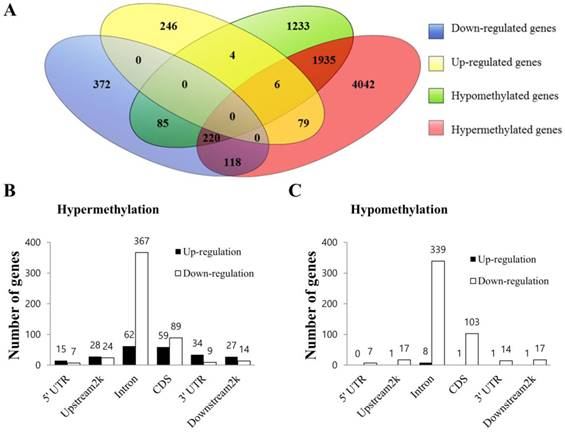
\includegraphics[width=0.8\textwidth]{journal-of-cancer_sample-result}}
	\caption{یک نمونه نمودار خلاصه برای نمایش نوآوری در نتایج
		%\cite{kim2016integrated}
	}
	\label{fig:sampleDiagram}
\end{figure}\\
طبیعتاً به صلاحدید نگارنده، شکل‌ها و نمودار‌ها می توانند در بخش های مختلف، خصوصا فصل
\ref{chap:results}
مورد استفاده قرار گیرند.

\subsection{تعریف واژه‌ها (اختیاری)}
در این قسمت محقق باید واژه‌هایی را که ممکن است برای خواننده آشنا نباشد، تعریف کند.

\subsection{خلاصه فصل‌ها}
در آخرین قسمتِ فصل اول پایان‌نامه، خلاصه‌ای اشاره‌وار از فصل‌های آتی آورده می‌شود تا خواننده بتواند تصویری واضح از دیگر قسمت‌های پایان‌نامه در ذهن خود ترسیم کند.

\section{جمع‌بندی}
در این فصل به دو مقولهٔ نحوه استفاده از قالب \پ دانشگاه تهران و نیز ویژگی‌هایی که محتویات فصل اول پایان‌نامه (یعنی مقدمه) باید داشته باشند، پرداخته شد. با توجه به اینکه این راهنما نحوه استفاده از قالب را شرح داده، ملزومات محتوایی هر فصل پایان‌نامه را توضیح می‌دهد و در پیوست‌ها نیز نحوهٔ کار با لاتک را یادآوری خواهد کرد، بنابراین مطالعهٔ کامل آن مقداری وقت شما را خواهد گرفت؛ اما مطمئن باشید از اتلاف وقت شما در ادامه کارتان تا حد زیادی جلوگیری خواهد کرد. در نوشتن متن حاضر سعی شده است علاوه بر ایجاد یک قالب لاتک برای پایان‌نامه‌های دانشگاه تهران، نکات محتوایی هر فصل نیز گوشزد گردد. طبیعتاً برای نگارش پایان‌نامهٔ خود می‌بایست مطالب تمام فصل‌ها را خودتان بازنویسی کنید.

در ادامهٔ این راهنما، تنها فصل‌هایی که یک پایان‌نامه باید داشته باشد و نیز خصوصیات یا ساختاری که محتویات هر فصل باید از آنها برخوردار باشد%
\footnote{از روی فایل «تمپلیت نگارش و تدوین پایان‌نامه \cite{UTThesisGuide}»}،
آورده می‌شوند. نهایتاً  در پیوست‌ها، مطالبی در باب یادآوری دستورات لاتک، نحوه نوشتن فرمول‌ها، تعاریف، قضایا، مثال‌ها، درج تصاویر، نمودارها، جداول و الگوریتم‌ها و نیز مدیریت مراجع، آمده است.

همچنین توصیه اکید دارم که رفع خطاهایی که احتمالاً با آنها مواجه می‌شوید را به آخر موکول نفرمایید و به محض برخورد با خطا، آن را اشکال‌زدایی و برطرف نمائید.!
و
\verb!% !TeX root=../main.tex
\setcounter{topnumber}{5}      % Increase number of floats at the top of the page
\setcounter{totalnumber}{5}    % Increase total number of floats on a page
\renewcommand{\floatpagefraction}{.8}  % Allow more of the page to be taken up by floats

\chapter{مروری بر مطالعات انجام شده}
%\thispagestyle{empty} 
\section{مقدمه}
در این فصل، پژوهش‌های پیشین در زمینه‌ی موتورهای مسطح مبتنی بر شناوری مغناطیسی (MLPM) با تمرکز بر ویژگی‌های اساسی آنان که به طور کلی در بخش‌های زیر دسته‌بندی شده‌اند، مورد بررسی قرار می‌گیرند. 
\begin{itemize}
	\item
		\textit{معماری دستگاه}:
بررسی انواع معماری‌های موجود برای MLPM و تأثیر آن‌ها بر عملکرد کلی سیستم.
	\item
		\textit{ساختار آهنرباهای دائمی و الکتریکی}:
مرور انواع آهنرباهای الکتریکی و چینش‌های مختلف آهنربا‌های دائمی و نقش آن‌ها در بهینه‌سازی عملکرد سیستم.
	\item
		\textit{طراحی کنترلر}:
معرفی روش‌های کنترل کلاسیک و مدرن برای این سیستم‌ها و چگونگی بهبود پایداری و دقت حرکت.
	\item
		\textit{روش‌های شناسایی سیستم و مدل‌سازی دینامیکی}:
تحلیل روش‌های شناسایی و تخمین مدل‌های دینامیکی سیستم برای شبیه‌سازی و بهینه‌سازی عملکرد.
\end{itemize}
در بخش‌های بعد، پژوهش‌های انجام‌شده بر اساس این ویژگی‌ها ارزیابی شده و مزایا و معایب هر روش مورد بررسی قرار می‌گیرد.

\section{معماری دستگاه‌های MLPM}
سیستم‌های شناوری مغناطیسی به دلیل ماهیت ناپایدارشان بدون استفاده از حلقه‌های کنترلی نمی‌توانند پایداری لازم را فراهم کنند. به همین دلیل، در تمامی ساختارهای پیشنهادی، از سیم‌پیچ‌های الکتریکی برای تولید میدان مغناطیسی با شدت کنترل ‌شده استفاده می‌شود. این سیم‌پیچ‌ها وظیفه دارند تا موقعیت جسم معلق را پایدار کرده و آن را در حالت مطلوب نگه ‌دارند.

در طراحی موتورهای مسطح، که از دو بخش ثابت
\LTRfootnote{Stator}
 و متحرک
\LTRfootnote{Mover}
تشکیل شده‌اند، امکان تغییر در طراحی و محل قرارگیری آهنرباهای الکتریکی و دائمی وجود دارد. نیروی مغناطیسی وارد بر بخش متحرک می‌تواند به‌صورت جاذبه‌ای از بالا یا دافعه‌ای از پایین اعمال شود. با این حال، در موتورهای مسطح به دلیل لزوم کم بودن فاصله میان سیم‌پیچ‌ها و اجسام معلق، اعمال نیروی جاذبه‌ای از بالا امکان‌پذیر نیست. به همین دلیل، در تمامی طراحی‌ها، نیروی مغناطیسی دافعه‌ای از سمت پایین به بخش متحرک وارد می‌شود که امکان جابه‌جایی اجسامی که بر روی آنها قرار می‌گیرند را فراهم می‌کند.

با توجه به این موارد، دو طراحی کلی برای ساخت دستگاه‌های MLPM ارائه می‌شود که در ادامه بررسی می‌‌شوند.
\subsection{سیم‌پیچ‌های متحرک و آهنرباهای ثابت}

در این معماری، بخش استاتور از مجموعه‌ای آهنربای ثابت تشکیل شده که میدان مغناطیسی پایدار در محیط اطراف خود ایجاد می‌کنند. بخش متحرک دستگاه شامل سیم‌پیچ‌هایی است که با عبور جریان الکتریکی از آن‌ها، میدان مغناطیسی متغیری تولید می‌گردد. این جریان به گونه‌ای تنظیم می‌شود که نیروی وارد بر آهنرباهای دائمی به‌دقت کنترل شود. طبق قانون سوم نیوتن، نیروهای وارد بر سیم‌پیچ‌ها و آهنرباهای دائمی به‌عنوان عمل و عکس‌العمل رفتار می‌کنند؛ به این ترتیب، نیرویی که به آهنرباها اعمال می‌شود، باعث ایجاد نیرویی برابر و در جهت مخالف بر سیم‌پیچ‌ها خواهد شد.

در پژوهش 
\cite{RN49}
، از ساختاری با سیم‌پیچ‌های چندلایه متعامد در بخش متحرک استفاده شده است. لایه اول سیم‌پیچ‌ها نیرویی را در راستاهای x و z ایجاد می‌کند، در حالی که لایه دوم نیرو را در راستاهای y و z اعمال می‌کند. این جداسازی نیروها به بهبود کنترل سیستم کمک می‌کند. علاوه بر این، به دلیل تفاوت فاصله میان لایه‌ها و استاتور، نیروهای تولیدشده توسط هر لایه متفاوت خواهند بود. راهکار ارائه‌شده برای این چالش، افزایش ضخامت لایه‌های دورتر از استاتور است. با این حال، برای جلوگیری از مشکلات ناشی از تفاوت ضخامت لایه‌ها، ساختاری سه‌لایه طراحی شده که ضمن افزایش نیروی تولیدی، ضخامت یکنواختی را در تمامی راستاها فراهم می‌نماید. در شکل 
\ref{fig:Multilayer_Mover_Coil}
ساختار این دستگاه نمایش داده شده است.

در پژوهش 
\cite{RN38}
، بخش متحرک از یک لایه سیم‌پیچ با چینش متعامد تشکیل شده که قابلیت اعمال نیرو در سه راستا را فراهم می‌سازد. در ادامه، پژوهش
\cite{RN14}
 روشی تحلیلی برای بهینه‌سازی ضخامت این سیم‌پیچ‌ها ارائه کرده است که با در نظر گرفتن معیارهای مختلف، به بهبود عملکرد سیستم می‌پردازد. شکل 
\ref{fig:Single_layer_Mover_Coil}
 این ساختار را نمایش داده است.

\begin{figure}[ht]
\centering 
\subfloat[استفاده از سیم‌پیچ‌های چندلایه
\cite{RN49}]
{ \label{fig:Multilayer_Mover_Coil}
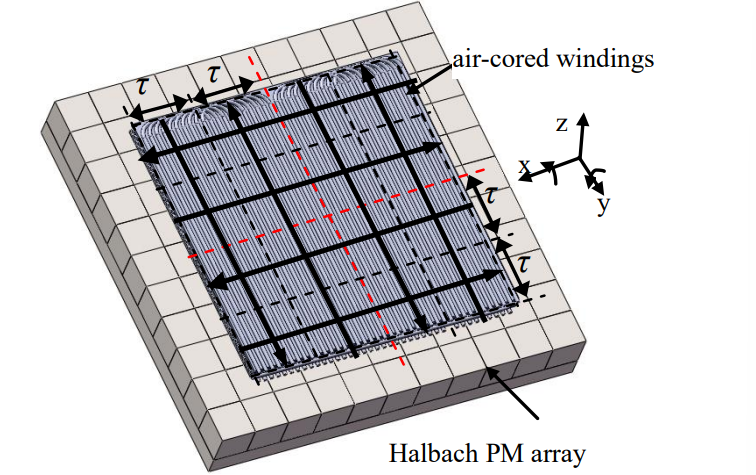
\includegraphics[width=0.5\textwidth]{Multilayer_Mover_Coil}}
%\hspace{2mm}
\subfloat[استفاده از سیم‌پیچ‌های یک لایه متعامد
\cite{RN14}]
{ \label{fig:Single_layer_Mover_Coil}
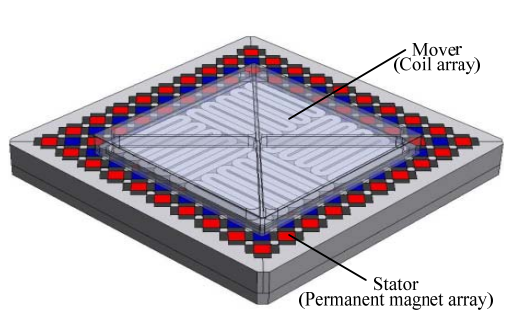
\includegraphics[width=0.5\textwidth]{Single_layer_Mover_Coil}}%
\caption{ساختار سیستم‌های MLPM با سیم‌پیچ‌های متحرک و آهنربای ثابت}
\label{fig:Moveing_Coil} %% label for entire figure
\end{figure}

با وجود اینکه این معماری امکان دستیابی به شناوری پایدار و حرکت با شش درجه آزادی را فراهم می‌کند، اما در کاربردهای عملی با محدودیت‌هایی مواجه است که بر عملکرد نهایی سیستم تأثیرگذار هستند. نخستین محدودیت، نیاز به تأمین انرژی الکتریکی برای سیم‌پیچ‌ها از طریق سیم‌های فیزیکی است که این امر به‌طور اجتناب‌ناپذیری ارتباط فیزیکی میان جسم متحرک و محیط اطراف را برقرار می‌سازد، در نتیجه حرکت آزادانه کامل جسم متحرک محدود می‌شود. دومین محدودیت، چالش خنک‌کاری سیم‌پیچ‌ها است که به دلیل ماهیت متحرک و معلق بودن آن‌ها، اجرای یک سیستم خنک‌کننده کارآمد دشوار خواهد بود. این مشکلات، نیاز به ارائه معماری جدیدی را آشکار می‌کند که بتواند این چالش‌ها را برطرف سازد.

\subsection{‌آهنرباهای متحرک و سیم‌پیچ‌های ثابت}

معماری دیگری که برای طراحی دستگاه‌های MLPM ارائه شده است، شامل قرار دادن سیم‌پیچ‌ها در بخش استاتور و استفاده از آهنرباهای دائمی در بخش متحرک می‌باشد. این ساختار نوین که در بسیاری از پژوهش‌ها مورد استفاده قرار گرفته، مشکلات معماری‌های پیشین مانند محدودیت جابه‌جایی متحرک ناشی از اتصالات فیزیکی و چالش‌های خنک‌کاری سیم‌پیچ‌ها را برطرف کرده و منجر به بهبود عملکرد کلی سیستم شده است.

در پژوهش 
\cite{RN7}
 استاتوری با چینش سیم‌پیچ‌ها مطابق با الگوی شاه‌ماهی
\LTRfootnote{Herringbone pattern}
 طراحی و پیاده‌سازی شده است. این طراحی امکان اعمال نیروی مغناطیسی به دو آهنربای دیسکی تعبیه‌شده در بخش متحرک را فراهم کرده است که دقتی در حدود 1 درجه در زوایای حرکت و 1 میلی‌متر در موقعیت متحرک به دست آورده است
\cite{RN7}
. در ادامه این پژوهش، ساختاری جدید برای بخش متحرک ارائه شده که شامل 6 آهنربای دیسکی با چینش کروی و فواصل ثابت می‌باشد. این طراحی توانسته است چرخش آزادانه متحرک را حول سه محور ممکن سازد 
\cite{RN39}.
شکل (
\ref{fig:Moving_Magnet_1})
همچنین در پژوهش 
\cite{RN62}
 نیز از این چینش سیم‌پیچ‌ها استفاده شده و مطابق با شبیه‌سازی‌های ارائه شده، مزیت آنان در ایجاد میدان مغناطیسی یکنواخت‌تر در نواحی کناری سیم‌پیچ‌ها نمایش داده شده است.

استفاده از سیم‌پیچ‌های سه‌فاز به‌جای تغذیه با جریان مستقیم، رویکردی است که در پژوهش 
\cite{RN24}
معرفی و اجرا شده است. در این ساختار، چهار آرایه از سیم‌پیچ‌های سه‌فاز، همان‌طور که در 
شکل (
\ref{fig:Moving_Magnet_2})
 نشان داده شده است، به‌گونه‌ای طراحی شده‌اند که نیروی مغناطیسی لازم را تولید کنند.

به ‌منظور کاهش هزینه‌ی محاسباتی در جابه‌جایی‌های طولانی، پژوهش 
\cite{RN32}
 ساختاری را ارائه کرده است که از دو مجموعه سیم‌پیچ‌ سه‌فاز و تک‌فاز تشکیل شده است. در این طراحی، کنترل حرکت در مسافت‌های طولانی توسط سیم‌پیچ‌های سه‌فاز انجام می‌پذیرد، در حالی که برای تنظیم دقیق موقعیت متحرک در صفحه، از سیم‌پیچ‌های تک‌فاز بهره برده می‌شود.
شکل (
\ref{fig:Moving_Magnet_3})

استفاده از سیم‌پیچ‌های ماژولار در طراحی استاتورهایی با چینش دوبعدی، رویکردی است که در دستگاه‌های MagTable و MagFloor از دانشگاه واترلو پیاده‌سازی شده است
\cite{RN8,RN30,RN10}
 در این طراحی، ماژول‌هایی از سیم‌پیچ‌های با سطح مقطع مربع به‌گونه‌ای طراحی شده‌اند که با قرار گرفتن در کنار یکدیگر، فضای کاری نامحدودی برای جابه‌جایی متحرک فراهم می‌کنند.(شکل
\ref{fig:Moving_Magnet_4})
 همچنین، پژوهش
\cite{RN8}
 نشان داده است که آهنرباهای با سطح مقطع مربع، در مقایسه با سیم‌پیچ‌های دایروی با جریان الکتریکی مشابه، می‌توانند شدت میدان مغناطیسی بیشتری ایجاد کنند، که این مزیت عملکرد کلی سیستم را بهبود می‌بخشد.

\begin{figure}[ht]
\centering 
\subfloat[الگوی شاه‌ماهی سیم‌پیچ‌ها
\cite{RN39}]
{ \label{fig:Moving_Magnet_1}
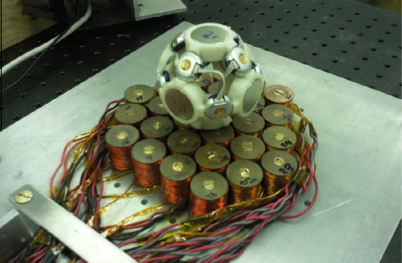
\includegraphics[width=0.45\textwidth]{Moving_Magnet_1}}
\hspace{2mm}
\subfloat[سیم‌پیچ‌های سه فاز
\cite{RN24}]
{ \label{fig:Moving_Magnet_2}
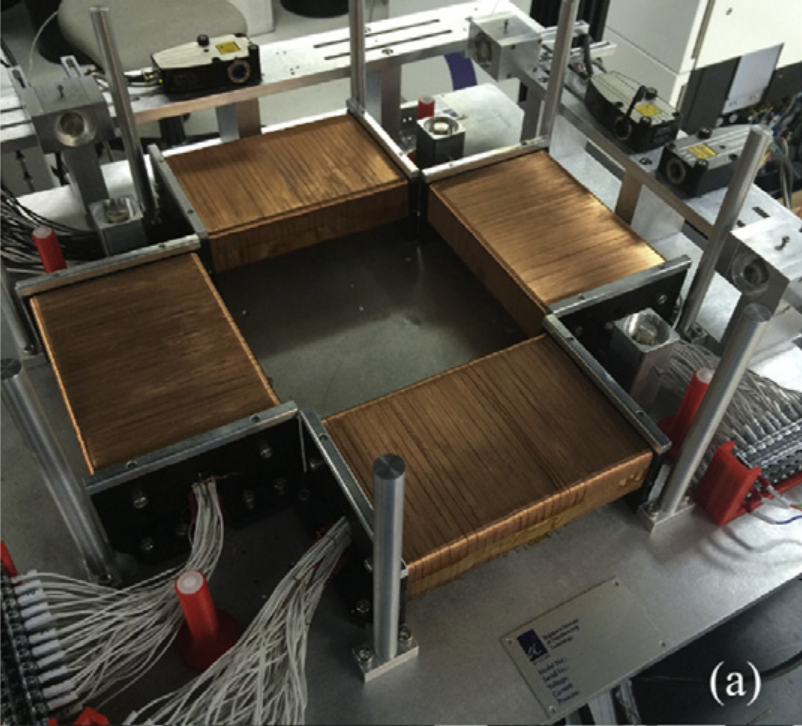
\includegraphics[width=0.45\textwidth]{Moving_Magnet_2}}
\\ % Newline to wrap the figures to the next row
\subfloat[ساختار دوگانه سیم‌پیچ‌ها
\cite{RN32}]
{ \label{fig:Moving_Magnet_3}
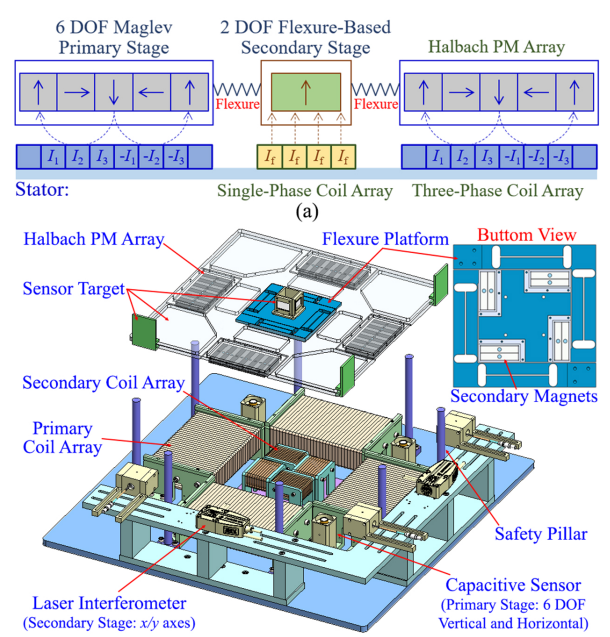
\includegraphics[width=0.45\textwidth]{Moving_Magnet_3}}
\hspace{2mm}
\subfloat[ساختار ماژولار سیم‌پیچ‌ها
\cite{RN10}]
{ \label{fig:Moving_Magnet_4}
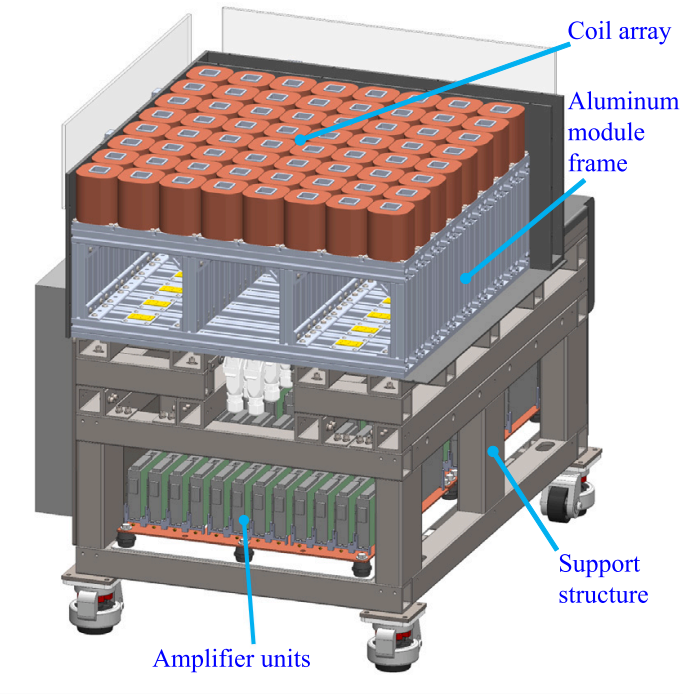
\includegraphics[width=0.45\textwidth]{Moving_Magnet_4}}
\label{fig:Moveing_Magnet} %% label for entire figure
\caption{ساختارهای آهنرباهای متحرک و سیم‌پیچ‌های ثابت}
\end{figure}








\section{ساختار آهنرباهای دائمی}

همان‌طور که در بخش قبل اشاره شد، میدان مغناطیسی کنترل‌شده توسط آهنرباهای الکتریکی ایجاد می‌شود و بر اثر تعامل این میدان متغیر با میدان ثابت آهنرباهای دائمی، نیرویی بر بخش متحرک دستگاه وارد می‌شود که حرکت آن را در راستاهای مختلف ممکن می‌سازد. بنابراین، طراحی بهینه آهنرباهای دائمی، به‌ویژه برای تولید میدان مغناطیسی قوی‌تر با کمترین وزن، در بهبود کارایی دستگاه نقش کلیدی دارد. در این بخش، طراحی‌های مختلف آهنرباهای دائمی که در پژوهش‌های پیشین ارائه شده‌اند، با تمرکز بر بهینه‌سازی این ویژگی‌ها بررسی می‌شوند.
\subsection{استفاده از آهنرباهای دیسکی}

استفاده از آهنرباهای دیسکی رویکردی ساده و مؤثر برای ایجاد میدان مغناطیسی دائمی محسوب می‌شود. با انتخاب موادی با خاصیت مغناطیسی بالا، مانند آهنرباهای نئودیمیومی، می‌توان به شدت میدان مغناطیسی مطلوب دست یافت. به عنوان نمونه، در پژوهش 
\cite{RN7}
 از دو آهنربای دیسکی جهت تأمین میدان مغناطیسی ثابت استفاده شده است. همچنین در پژوهش 
\cite{RN39}
 با به‌کارگیری ۶ آهنربای دیسکی، امکان چرخش آزادانه حول سه محور فراهم شده است.(شکل
\ref{fig:Disk_Magnet_1})
 در پژوهش 
\cite{RN8}
 نیز از ترکیب‌های متفاوتی از آهنرباهای دیسکی برای بخش متحرک دستگاه استفاده شده است، که این ترکیب‌ها شامل تغییر اندازه‌ی یک آهنربا و استفاده از سه آهنربای دیسکی است. سیستم شناوری مغناطیسی با پنج درجه آزادی که تنها از یک آهنربای دیسکی تشکیل شده است، در پژوهش 
\cite{RN62}
 به عنوان نمونه‌ای موفق از این رویکرد معرفی شده است. این طراحی، با وجود سادگی معماری، توانسته نتایج رضایت‌بخشی را از نظر عملکرد ارائه دهد و نشان می‌دهد که استفاده از آهنربای دیسکی، علاوه بر سادگی، می‌تواند در کاربردهای مختلف به‌ویژه در سیستم‌های با نیاز به دقت بالا و چند درجه آزادی، کارآمد باشد. شکل((
\ref{fig:Disk_Magnet_2})


\begin{figure}[ht]
\centering 
\subfloat[دو آهنربای دیسکی
\cite{RN7}]
{ \label{fig:Disk_Magnet_1}
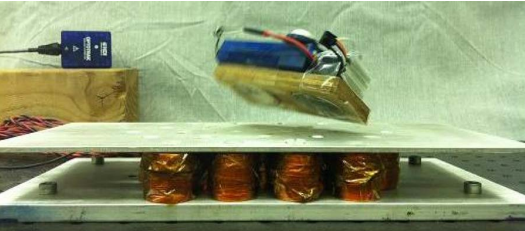
\includegraphics[width=0.5\textwidth]{Disk_Magnet_1}}
%\hspace{2mm}
\subfloat[یک آهنربای دیسکی
\cite{RN62}]
{ \label{fig:Disk_Magnet_2}
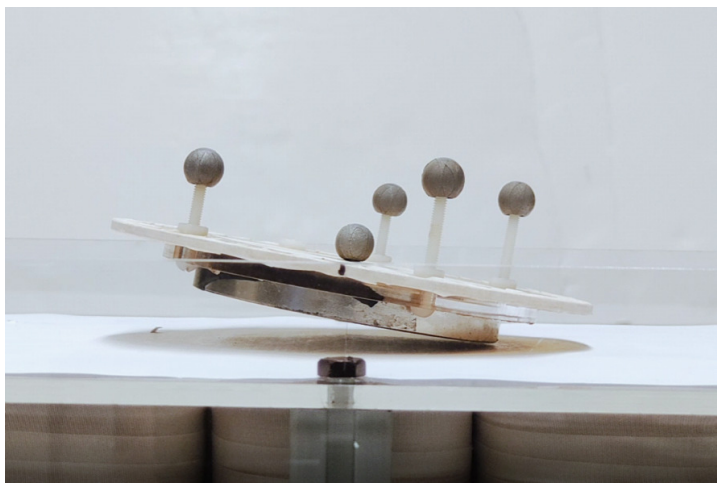
\includegraphics[width=0.5\textwidth]{Disk_Magnet_2}}%
\caption{استفاده از آهنربای دیسکی در طراحی متحرک}
\label{fig:Disk_Magnet} %% label for entire figure
\end{figure}



\subsection{آرایه‌ی هالباخ یک بعدی}

آرایه‌ی هالباخ
\LTRfootnote{Halbach Array}
 به‌عنوان چینشی از آهنرباهای دائمی تعریف می‌شود که در آن جهت مغناطیس‌شوندگی هر آهنربا با آهنربای مجاور خود ۹۰ درجه تفاوت دارد. این آرایه به‌طور خاص قادر است میدان مغناطیسی در یک سوی آرایه را خنثی کرده و در سوی دیگر میدان را به میزان تقریبی 1.4 برابر افزایش دهد.
مزیت این ساختار در طراحی سیستم‌های MLPM، توانایی آن در تولید شدت میدان مغناطیسی بیشتر است. به‌همین‌دلیل، این چینش در بسیاری از پژوهش‌ها مورد استفاده قرار گرفته است.
با این حال، استفاده از تنها یک آرایه‌ی یک‌بعدی هالباخ به‌تنهایی نمی‌تواند نیرویی در دو راستای افقی ایجاد کند. لذا معمولاً از تعداد بیشتری از این آرایه‌ها در ساختار متحرک استفاده می‌شود. به‌عنوان مثال، در پژوهش‌های 
\cite{RN24,RN27}
 از چهار آرایه‌ی هالباخ یک‌بعدی در بخش متحرک استفاده شده است که هر یک از این آرایه‌ها قادر به ایجاد نیرویی در یکی از راستاهای افقی و عمودی هستند.
در پژوهش 
\cite{RN39}
، مشابه آنچه که در بخش استاتور پیاده‌سازی شده بود، از ساختار دوگانه‌ای در بخش متحرک بهره‌برداری شده است، به‌گونه‌ای که دو مجموعه چهارگانه از آرایه‌های هالباخ در معماری این بخش به‌کار رفته‌اند.

\begin{figure}[ht]
\centering 
\subfloat[آرایه‌ی هالباخ
\cite{RN16}]
{ \label{fig:halbach1D}
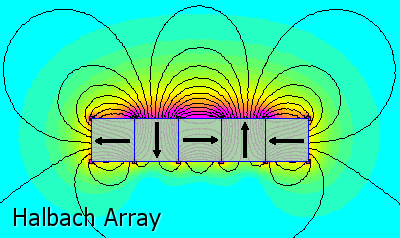
\includegraphics[width=0.5\textwidth]{halbach1D}}
%\hspace{2mm}
\subfloat[4 آرایه‌ی یک بعدی هالباخ
\cite{RN39}]
{ \label{fig:4_halbach1D_array}
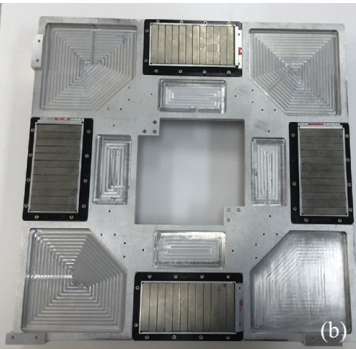
\includegraphics[width=0.5\textwidth]{4_halbach1D_array}}%
\caption{آرایه هالباخ یک‌بعدی}
\label{fig:halbach1D} %% label for entire figure
\end{figure}

\subsection{آرایه هالباخ دوبعدی}

برای رفع محدودیت‌های آرایه‌ی هالباخ یک‌بعدی که تنها در یک راستا نیرو ایجاد می‌کند، ساختار جدیدی از آرایه‌ی دوبعدی ارائه شده است. این آرایه قادر است میدان مغناطیسی را در یک طرف صفحه حذف و در طرف دیگر تقویت کند. با این ویژگی، استفاده از چندین آرایه برای تأمین میدان مغناطیسی ثابت ضروری نخواهد بود. طراحی آرایه‌ی دوبعدی در بسیاری از پژوهش‌ها برای بخش‌های متحرک یا استاتور سیستم‌های MLPM به کار گرفته شده است.

استفاده از آرایه‌ی هالباخ در پژوهش‌های مختلفی از جمله
\cite{RN10, RN30} 
و
\cite{RN55, RN26} 
نشان‌دهنده‌ی عملکرد بهینه‌ی این معماری در بخش متحرک سیستم‌های MLPM است.(شکل
\ref{fig:halbach2D_2})
 همچنین در پژوهش
\cite{RN14}
 از این آرایه به عنوان بخشی از استاتور دستگاه بهره‌گیری شده است. در 
\cite{RN61}
 ماژول‌هایی برای ساخت این آرایه استفاده شده (شکل
\ref{fig:halbach2D_4})
 و در
\cite{RN49}
 برای تشکیل آرایه از قطعات آهنی در فضای خالی میان آن استفاده شده است؛ اما این رویکرد باعث ایجاد خطا در دقت میدان مغناطیسی شده است. (شکل
\ref{fig:halbach2D_3})
علاوه بر این، در پژوهش
\cite{RN28}
، طراحی جدیدی با آهنرباهایی با میزان مغناطیس‌شوندگی و ارتفاع متفاوت پیشنهاد شده است.
\begin{figure}[ht]
\centering 
\subfloat[آرایه هالباخ دو بعدی و میدان مغناطیسی آن
\cite{RN10}]
{ \label{fig:halbach2D_2}
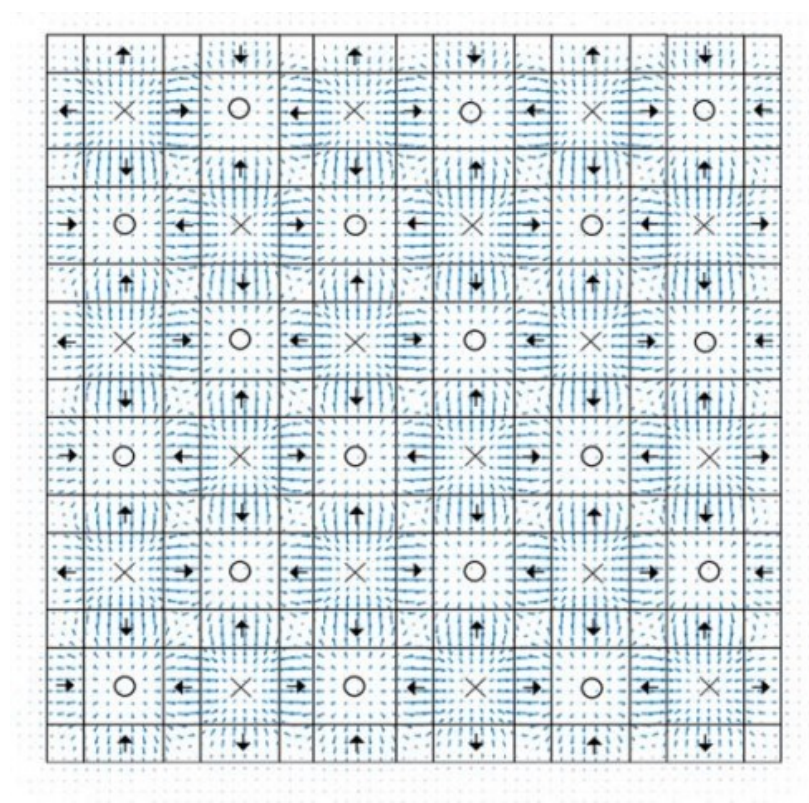
\includegraphics[width=0.45\textwidth]{halbach2D_2}}
\hspace{2mm}
\subfloat[آرایه هالباخ دوبعدی با قطعات آهنی در فضاهای خالی
\cite{RN49}]
{ \label{fig:halbach2D_3}
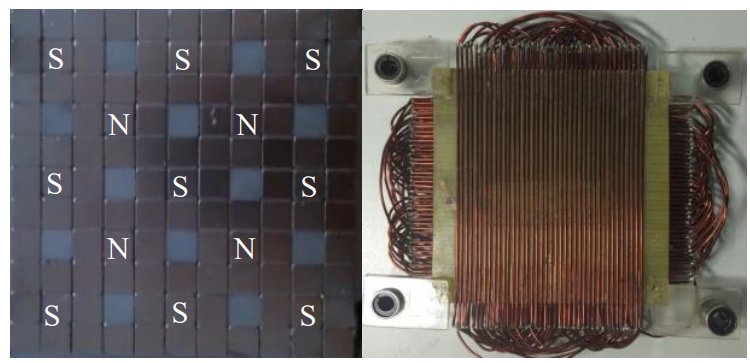
\includegraphics[width=0.45\textwidth]{halbach2D_3}}
\\ % Newline to wrap the figures to the next row
\subfloat[آرایه هالباخ دوبعدی ماژولار
\cite{RN61}]
{ \label{fig:halbach2D_4}
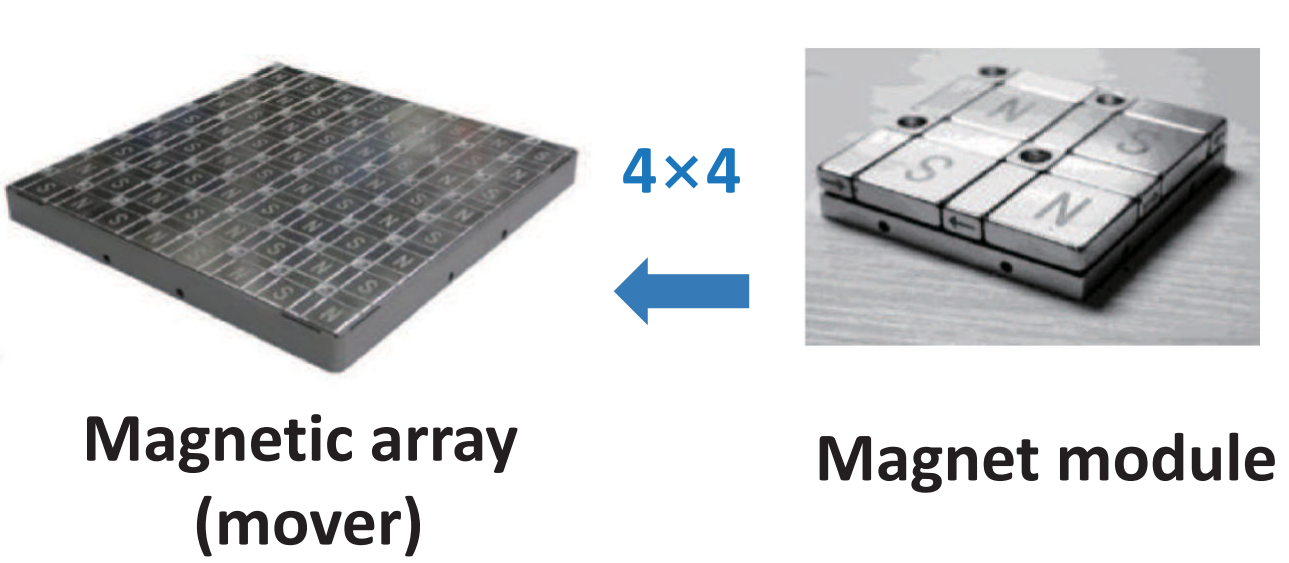
\includegraphics[width=0.45\textwidth]{halbach2D_4}}
\caption{آرایه هالباخ دو‌بعدی}
\label{fig:halbach2D} %% label for entire figure

\end{figure}
\section{طراحی کنترلر}
همان‌طور که پیش‌تر اشاره شد، سیستم‌های شناوری مغناطیسی ذاتاً ناپایدار هستند و برای دستیابی به پایداری، به کنترلری با عملکرد دقیق و خطای کم نیاز است. در پژوهش‌های مختلف، از کنترلرهای گوناگونی برای این سیستم‌ها بهره گرفته شده است؛ از جمله کنترلرهای کلاسیک نظیر PID، کنترلرهای مدرن مانند کنترل مبتنی بر پیش‌بینی مدل (MPC) و همچنین مدل‌های مبتنی بر هوش مصنوعی نظیر شبکه‌های بازگشتی GRU. در این بخش، به بررسی این کنترلرها و مقایسه‌ عملکرد آنها خواهیم پرداخت.
\subsection{کنترلر PID}

کنترل تناسبی-انتگرالی-مشتقی (PID) به عنوان یکی از پرکاربردترین و موثرترین کنترلرهای کلاسیک در سیستم‌های دینامیکی، گزینه‌ای مناسب برای کنترل سیستم‌های MLPM محسوب می‌شود. این کنترلر به دلیل سادگی در پیاده‌سازی، تنظیم دقیق و توانایی تنظیم خروجی سیستم بر اساس خطاهای ورودی، به‌طور گسترده در سیستم‌های مختلف استفاده شده است. برای کنترل سیستم‌های MLPM، به ازای هر درجه آزادی یک کنترلر PID طراحی و پیاده‌سازی می‌شود تا بتواند جریان الکتریکی سیم‌پیچ‌ها را تنظیم کرده و میدان مغناطیسی لازم برای ایجاد و حفظ موقعیت متحرک را تأمین کند.

در پژوهش‌های متعددی از کنترلر PID برای سیستم‌های MLPM بهره گرفته شده است. به عنوان مثال، در 
\cite{RN39,RN24}
از کنترلرهای PID ساده برای کنترل جریان سیم‌پیچ‌ها استفاده شده که وظیفه تنظیم میدان مغناطیسی و در نتیجه، کنترل موقعیت جسم متحرک را بر عهده دارند. علاوه بر این، در پژوهش
\cite{RN32}
، از دو کنترلر PID در یک ساختار دوگانه استفاده شده است. کنترلر اول برای جابه‌جایی‌های بلند و در مسافت‌های طولانی به کار رفته و جریان سیم‌پیچ‌های اصلی را تنظیم می‌کند، در حالی که کنترلر دوم برای حرکات دقیق کوتاه‌برد طراحی شده و کنترل جریان سیم‌پیچ‌های ثانویه را بر عهده دارد. این روش باعث بهینه‌سازی کنترل دقیق و بهبود دقت در حرکات کوتاه‌برد و جابه‌جایی‌های سریع می‌شود.
همچنین در سیستم MagTable، برای کنترل دقیق موقعیت آهنرباهای دائمی، از شش کنترلر PID به‌صورت همزمان استفاده شده است تا نیروی متوازن برای پایدارسازی موقعیت متحرک در چندین جهت فراهم شود 
\cite{RN8}
. این نوع طراحی و استفاده از کنترلرهای PID نشان می‌دهد که علی‌رغم محدودیت‌های موجود در کنترلرهای کلاسیک، این روش همچنان در بسیاری از سیستم‌های مغناطیسی پیچیده مانند MLPM کارایی بالایی دارد.

\begin{figure}[ht]
\centering{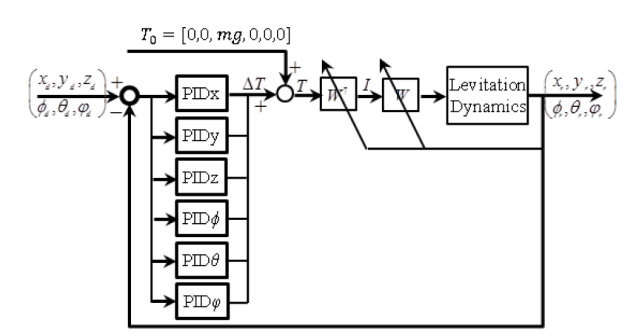
\includegraphics[width=0.5\textwidth]{PID_1}}
\caption{کنترلر PID با 6 درجه آزادی
\cite{RN8}}
\label{fig:PID}
\end{figure}


\subsection{کنترلر مبتنی بر پیش‌بینی مدل MPC}
برای کنترل سیستم‌های MLPM اگر مدل سیستم به روش‌های تحلیلی و یا عددی به دست آمده و تخمین زده شده باشد، می‌توان از این مدل‌ها برای طراحی کنترلرهای پیشرفته‌تر با هدف پیش‌بینی رفتار سیستم و استفاده از آن به صورت پیش‌خور در حلقه‌ی کنترلی استفاده کرد. روش‌های تخمین مدل این سیستم‌ها در بخش‌های بعد مورد بررسی قرار می‌گیرد. در این بخش، کنترلرهای ارائه شده در پژوهش‌های دیگر ارائه می‌شود.
به دست آوردن معادلات دینامیکی سیستم و استفاده از آنها در پیش‌بینی روشی تحلیلی است که در 
\cite{RN55}
 استفاده شده است و مدل کنترلی متشکل از بلوک‌های پس‌خور و پیش‌خور برای کنترل موقعیت آهنربا طراحی شده است. همچنین در 
\cite{RN62}
 از یک جدول جستجو برای تعیین رفتار سیستم در نقاط مختلف فضا استفاده شده است که این جدول به عنوان پیش‌خور به مدل کنترلی داده می‌شود. در ادامه‌ی این پژوهش، با استفاده از روش‌های شناسایی سیستم، مدلی تقریبی برای رفتار سیستم در نظر گرفته شده است و با استفاده از این مدل برای پیش‌بینی رفتار سیستم‌ مدل MPC پیاده‌سازی شده است. پژوهش 
\cite{RN30}
 با تمرکز بر ارائه‌ی یک مدل پیش‌بین، با استفاده از معادلات دینامیکی سیستم و همچنین روش‌پیش‌بینی حالت بی‌تاخیر، رفتار آینده‌ی سیستم را محاسبه می‌کند.
\begin{figure}[ht]
\centering 
\subfloat[\cite{RN55}]{
    \label{fig:MPC_1}
    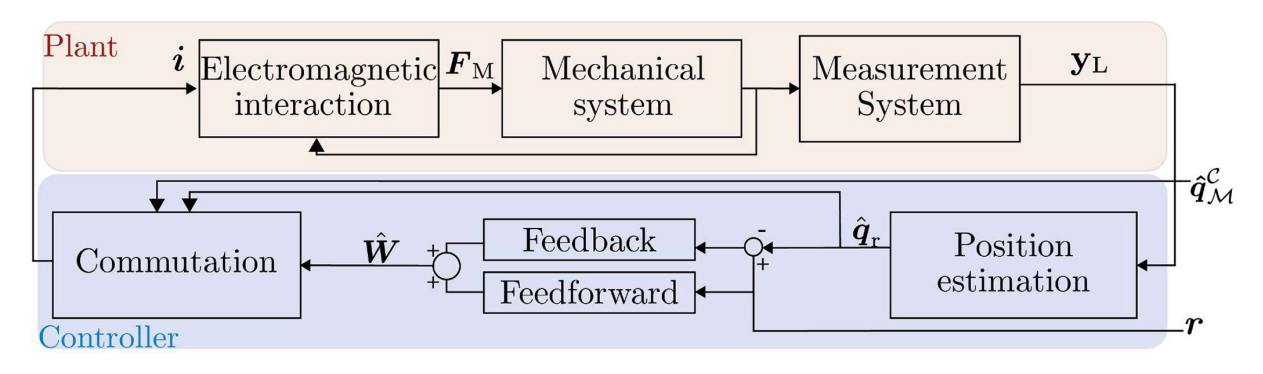
\includegraphics[width=0.45\textwidth]{MPC_1}}
%\hspace{2mm}
\subfloat[\cite{RN62}]{
    \label{fig:MPC_2}
    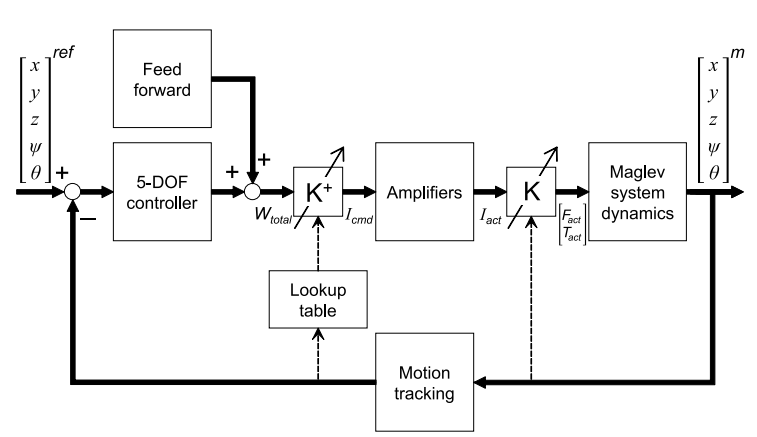
\includegraphics[width=0.45\textwidth]{MPC_2}}
\\ % Newline to wrap the figures to the next row
\subfloat[\cite{RN61}]{
    \label{fig:MPC_3}
    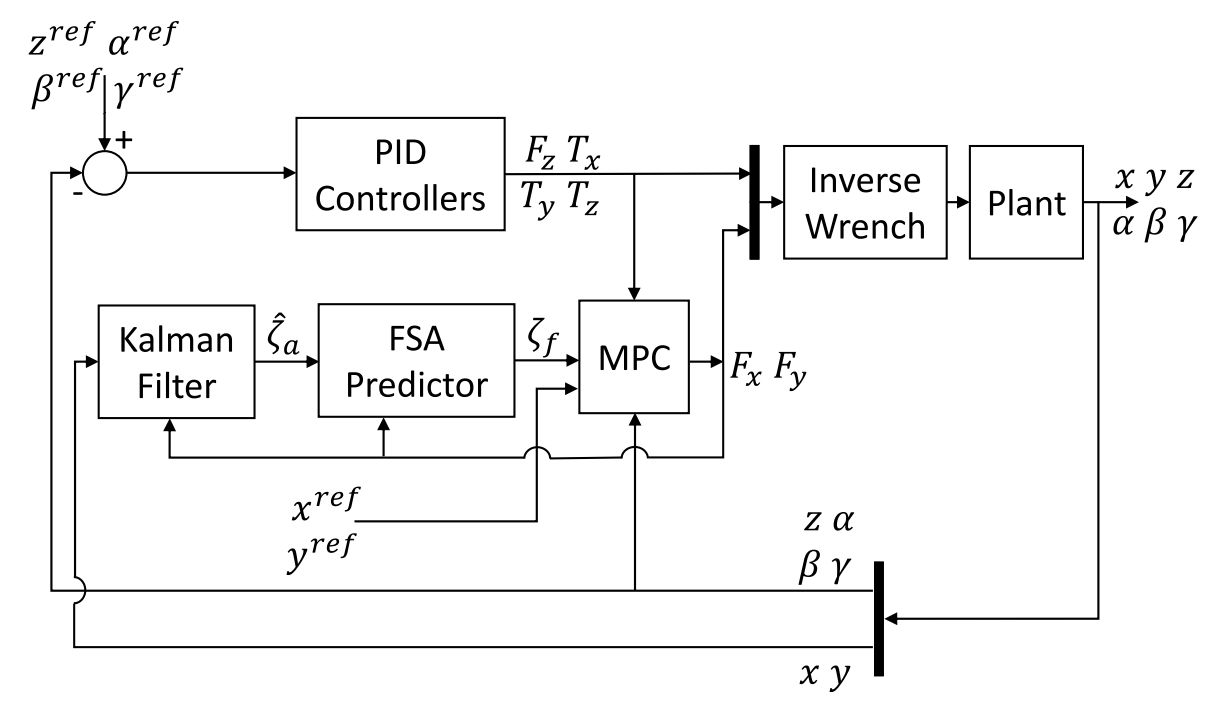
\includegraphics[width=0.45\textwidth]{MPC_3}}
\subfloat[\cite{RN61}]{
    \label{fig:MPC_4}
    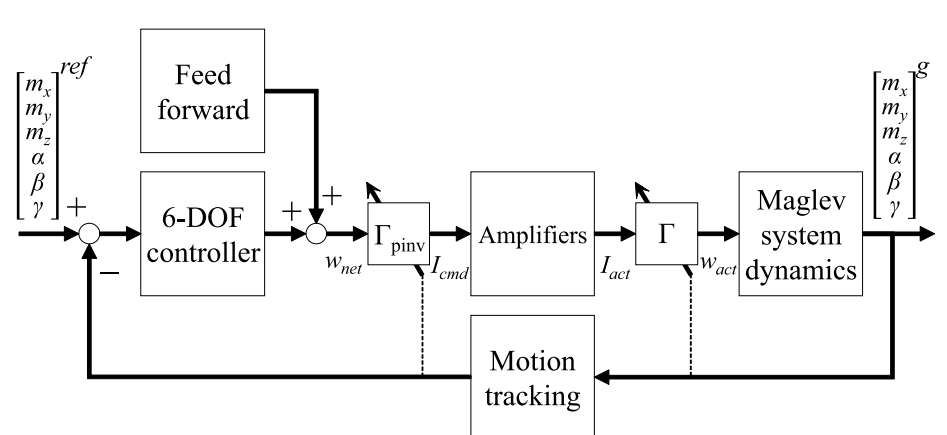
\includegraphics[width=0.45\textwidth]{MPC_4}}
\caption{کنترلر MPC}
\label{fig:MPC} %% label for entire figure
\end{figure}

\FloatBarrier

\subsection{کنترلر مبتنی بر هوش مصنوعی}

یکی از روش‌های نوین برای پیش‌بینی رفتار سیستم‌های پیچیده مانند MLPM، استفاده از مدل‌های هوش مصنوعی به‌ویژه شبکه‌های عصبی بازگشتی (RNN) است. این مدل‌ها با یادگیری دینامیک سیستم و ارتباط بین ورودی‌ها و خروجی‌ها، می‌توانند به‌طور مؤثری رفتار سیستم را در شرایط مختلف پیش‌بینی کنند. در این راستا، پژوهش
\cite{RN61}
از یک مدل بازگشتی GRU 
\LTRfootnote{Gated Recurrent Unit}
 استفاده کرده است. این مدل بر اساس داده‌های جمع‌آوری‌شده از عملکرد دستگاه MLPM آموزش دیده و توانسته است با دقت بالا تغییرات دینامیکی سیستم و پاسخ آن به ورودی‌های گوناگون را پیش‌بینی کند. استفاده از GRU به دلیل توانایی آن در مدل‌سازی وابستگی‌های زمانی و در نظر گرفتن اطلاعات قبلی برای پیش‌بینی‌های دقیق‌تر، رویکردی مناسب در این پژوهش بوده است.(شکل 
\ref{fig:GRU}

\begin{figure}[ht]
\centering
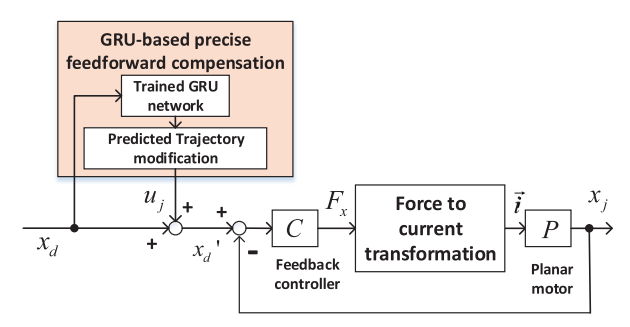
\includegraphics[width=0.5\textwidth]{GRU_1}
\caption{کنترلر پیش‌خور GRU \cite{RN61}}
\label{fig:GRU}
\end{figure}

\section{مدل‌سازی و تخمین سیستم}
در روش بار نقطه‌ای برای تحلیل میدان مغناطیسی، فرض می‌شود که توزیع بار مغناطیسی در یک حجم به‌صورت متمرکز در هشت نقطه در گوشه‌های آن حجم قرار گرفته است. با این فرض، اثر مغناطیسی این جسم می‌تواند به‌صورت مجموع آثار هر یک از بارهای نقطه‌ای محاسبه شود. این رویکرد امکان محاسبه‌ی دقیق شدت میدان مغناطیسی و نیروی وارد بر یک جسم خارجی را فراهم می‌آورد. از طریق محاسبه‌ی میدان‌های ناشی از هر بار نقطه‌ای و جمع آنها، میدان مغناطیسی کل حاصل می‌شود و به این ترتیب، شدت میدان مغناطیسی ناشی از آهنربای دائمی به کمک این روش به‌طور دقیق محاسبه می‌گردد. در ادامه، معادلات مربوط به محاسبه‌ی شدت میدان مغناطیسی ارائه شده‌اند.
\subsection{مدل بار مغناطیسی سطحی}
در این مدل، فرض بر این است که بار مغناطیسی در یک المان حجم سه‌بعدی به‌صورت توزیعی از بارهای مغناطیسی با چگالی بار J بر روی دو صفحه‌ی موازی قرار گرفته است. با استفاده از این فرض، میدان مغناطیسی ایجادشده توسط این حجم به‌صورت میدان حاصل از توزیع بارهای مغناطیسی محاسبه می‌شود. این مدل امکان تحلیل دقیق‌تر رفتار میدان مغناطیسی را فراهم می‌کند. مقایسه نتایج حاصل از این مدل با شبیه‌سازی المان محدود
\LTRfootnote{Finite Element Method (FEM)}
 در پژوهش
\cite{RN44}
نشان داده است که این روش مدل‌سازی برای سیستم‌های MLPM دقت و کارایی بالایی دارد.

\begin{figure}[ht]
\centering
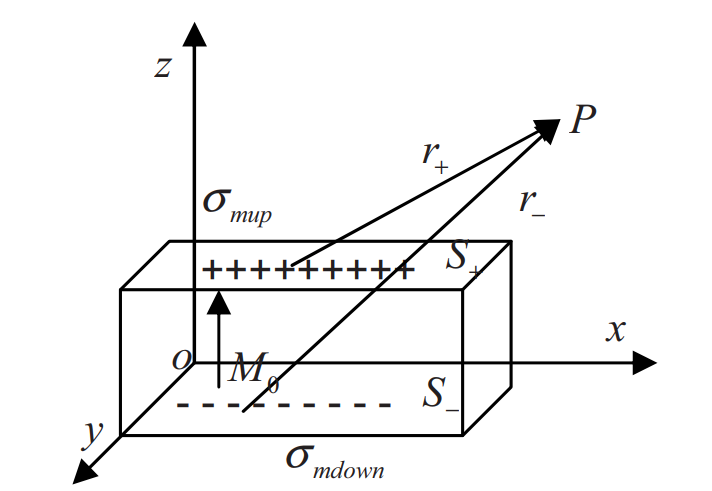
\includegraphics[width=0.5\textwidth]{Magnetic surface charge_2}
\caption{مدل بار مغناطیسی سطحی \cite{RN44}}
\label{fig:Magnetic surface charge}
\end{figure}

\subsection{مدل بار مغناطیسی نقطه‌ای}
در روش بار نقطه‌ای برای تحلیل میدان مغناطیسی، فرض می‌شود که توزیع بار مغناطیسی در یک حجم به‌صورت متمرکز در هشت نقطه در گوشه‌های آن حجم قرار گرفته است. با این فرض، اثر مغناطیسی این جسم می‌تواند به‌صورت مجموع آثار هر یک از بارهای نقطه‌ای محاسبه شود. این رویکرد امکان محاسبه‌ی دقیق شدت میدان مغناطیسی و نیروی وارد بر یک جسم خارجی را فراهم می‌آورد. از طریق محاسبه‌ی میدان‌های ناشی از هر بار نقطه‌ای و جمع آنها، میدان مغناطیسی کل حاصل می‌شود و به این ترتیب، شدت میدان مغناطیسی ناشی از آهنربای دائمی به کمک این روش به‌طور دقیق محاسبه می‌گردد. در ادامه، معادلات مربوط به محاسبه‌ی شدت میدان مغناطیسی ناشی از هر بار نقطه‌ای ارائه شده‌است.
\begin{align}
B_{xk} &= \frac{\epsilon_k}{4\pi} \ln\left(-y_r + \sqrt{x_r^2 + y_r^2 + z_r^2}\right), \\
B_{yk} &= \frac{\epsilon_k}{4\pi} \ln\left(-x_r + \sqrt{x_r^2 + y_r^2 + z_r^2}\right), \\
B_{zk} &= \frac{\epsilon_k}{4\pi} \arctan\left( \frac{x_r y_r}{\sqrt{x_r^2 + y_r^2 + z_r^2}} \right),
\end{align}

\begin{figure}[ht]
\centering
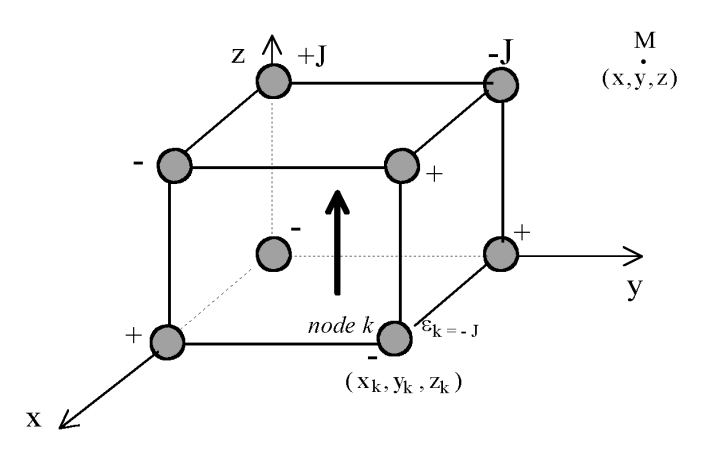
\includegraphics[width=0.5\textwidth]{Magnetic_Node}
\caption{مدل بار مغناطیسی نقطه‌ای \cite{RN44}}
\label{figMagnetic_Node}
\end{figure}

\subsection{مدل های مبتنی بر داده}

در این روش‌ها، به‌جای مدل‌سازی دقیق ساختار فیزیکی دستگاه و استخراج معادلات دینامیکی آن، پارامترهای مورد نیاز مانند شدت میدان مغناطیسی از طریق داده‌های تجربی یا شبیه‌سازی المان محدود (FEM) تخمین زده می‌شوند. این رویکرد مبتنی بر داده نیازمند دسترسی به اطلاعات دقیق از سیستم واقعی یا شبیه‌سازی کامل آن است تا بتوان دقت و اعتبار تخمین‌ها را ارزیابی کرد. در پژوهش 
\cite{RN10}
، برای تخمین شدت میدان مغناطیسی آرایه هالباخ دوبعدی از معادلات هارمونیک و سری فوریه استفاده شده است. تغییرات میدان مغناطیسی تولیدشده توسط این آرایه به‌صورت موجی سینوسی مدل‌سازی شده است، اما این روش تنها زمانی دقیق است که فرض شود سطح آرایه به‌صورت نامحدود ادامه دارد. برای حل این مشکل، آرایه به سه ناحیه مرکزی، کناری و گوشه‌ای تقسیم‌بندی شده و برای هر ناحیه هارمونیک‌های مجزا در نظر گرفته شده است. نتایج این پژوهش نشان می‌دهند که با استفاده از سه هارمونیک اول، می‌توان میدان مغناطیسی را در نواحی کناری و گوشه‌ای با دقت مناسبی تخمین زد.

\begin{figure}[ht]
\centering 
\subfloat[\cite{RN10}]{
\label{fig:harmonic_1}
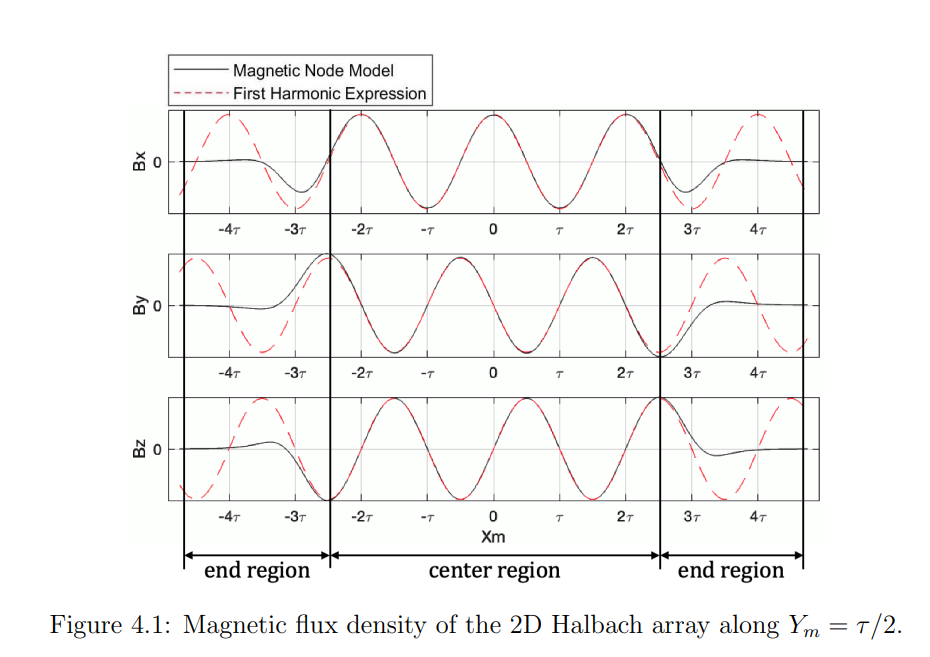
\includegraphics[width=0.45\textwidth]{harmonic_1}}
\hspace{2mm}
\subfloat[\cite{RN10}]{
\label{fig:harmonic_2}
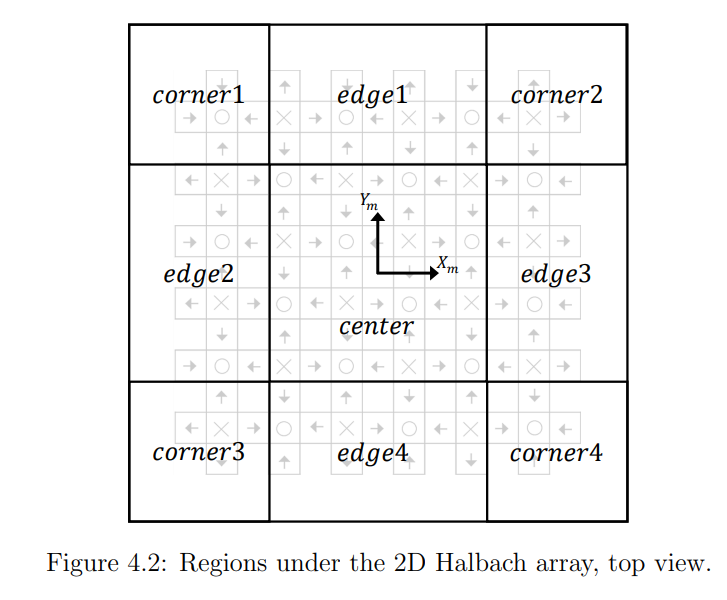
\includegraphics[width=0.45\textwidth]{harmonic_2}}
\caption{مدل هارمونیک}
\label{fig:harmonic}
\end{figure}



!
را در فایل 
\lr{main.tex}،
غیرفعال%
\footnote{
برای غیرفعال کردن یک دستور، کافی است در ابتدای آن، علامت درصد انگلیسی (\%) بگذارید.
}
 کنید. در غیر این صورت، ابتدا مطالب دو فصل اول پردازش شده و سپس مطالب فصل ۳ پردازش می‌شود که این کار باعث طولانی شدن زمان پردازش می‌گردد. هر زمان که خروجی کل \پ را خواستید، تمام فصل‌ها را دوباره در
\lr{main.tex}
فعال نمائید.
بدیهتاً لازم نیست فصل‌های \پ را به ترتیب تایپ کنید. مثلاً می‌توانید ابتدا مطالب فصل ۳ را تایپ نموده و سپس مطالب فصل ۱ را تایپ کنید. 
\subsubsection{مراجع}
برای وارد کردن مراجع \پ کافی است فایل 
\lr{MyReferences.bib}
را باز کرده و مراجع خود را به شکل اقلام نمونهٔ داخل آن، وارد کنید.  سپس از \lr{bibtex} برای تولید مراجع با قالب مناسب استفاده نمائید. برای توضیحات بیشتر بخش \ref{Sec:Ref} از پیوست \ref{app:latexIntro} و نیز پیوست \ref{app:refMan} را ببینید.

\subsubsection{واژه‌نامه فارسی به انگلیسی و برعکس}
برای وارد کردن معادل فارسی اصطلاحات لاتین در متن و تهیه فهرست واژه‌نامه از آنها، از بستهٔ
\lr{glossaries}
و نرم‌افزار
\lr{xindy}
استفاده می‌شود. بدین منظور کافی است اصطلاحات لاتین و ترجمهٔ آنها را در فایل
\lr{words.tex}
وارد کرده و هر جای متن که خواستید با دستورات
\verb|gls{label}|
یا \verb|glspl{label}|
معادل فارسی مفرد یا جمع یک اصطلاح را بیاورید.

مثلا در اینجا، واژهٔ
«\gls{Action}»
برای بار اول و دوباره
«\gls{Action}»
برای بار دوم در متن ظاهر شده است.
جهت توضیحات بیشتر به پیوست
\ref{app:refMan}
مراجعه کنید.
\subsubsection{نمایه}
برای وارد کردن نمایه، باید از 
\lr{xindy}
استفاده کنید. 
%زیرا 
%\lr{MakeIndex}
%با حروف «گ»، «چ»، «پ»، «ژ» و «ک» مشکل دارد و ترتیب الفبایی این حروف را رعایت نمی‌کند. همچنین، فاصله بین هر گروه از کلمات در 
%\lr{MakeIndex}،
%به درستی رعایت نمی‌شود که باعث زشت شدن حروف‌چینی این قسمت می‌شود. 
راهنمای چگونگی کار با 
\lr{xindy} 
را می‌توانید در ویکی پارسی‌لاتک و یا مثالهای موجود در دی‌وی‌دی «مجموعه پارسی‌لاتک»، پیدا کنید.

\subsection{اگر سوالی داشتم، از کی بپرسم؟}
برای پرسیدن سوال‌های خود موقع حروف‌چینی با زی‌پرشین، می‌توانید به
\href{http://qa.parsilatex.com}{سایت پرسش و پاسخ پارسی‌لاتک}%
\LTRfootnote{http://qa.parsilatex.com}
یا
\href{http://forum.parsilatex.com}{بایگانی تالارگفتگوی قدیمی پارسی‌لاتک}%
\LTRfootnote{http://forum.parsilatex.com}
مراجعه کنید. شما هم می‌توانید روزی به سوال‌های دیگران در اینترنت جواب دهید.
بستهٔ زی‌پرشین و بسیاری از بسته‌های مرتبط با آن مانند
\lr{bidi} و
\lr{Persian-bib}،
مجموعه پارسی‌لاتک، مثالهای مختلف موجود در آن، قالب پایان‌نامه دانشگاههای مختلف و سایت پارسی‌لاتک همه به صورت داوطلبانه توسط افراد گروه پارسی‌لاتک و گروه
\lr{Persian TeX}
و بدون هیچ کمک مالی انجام شده‌اند. کار اصلی نوشتن و توسعه زی‌پرشین توسط آقای وفا خلیقی انجام شده است که این کار بزرگ را به انجام رساندند.
اگر مایل به کمک به گروه پارسی‌لاتک هستید به سایت این گروه مراجعه فرمایید:
\begin{center}
	\url{http://www.parsilatex.com}
\end{center}

\section{محتویات فصل اول یک پایان‌نامه}
فصل اول یک پایان‌نامه باید به مقدمه یا کلیات تحقیق بپردازد.
هدف از فصل مقدمه%
\LTRfootnote{Introduction}،
شرح مختصر مسأله تحقیق، اهمیت و انگیزه محقق از پرداختن به آن موضوع، بهمراه اشاره‌ای کوتاه به روش و مراحل تحقیق است. مقدمه، اولین فصل از ساختار اصلی \پ بوده و زمینه اطلاعاتی لازم را برای خواننده فراهم می‌آورد. در طول مقدمه باید سعی شود موضوع تحقیق با زبانی روشن، ساده و بطور عمیق و هدفمند به خواننده معرفی شود. این فصل باید خواننده را مجذوب و اهمیت موضوع تحقیق را آشکار سازد. در مقدمه باید با ارائهٔ سوابق، شواهد تحقیقی و اطلاعات موجود (با ذکر منبع) با روشی منظم، منطقی و هدف‌دار، خواننده را جهت داد و به سوی راه حل مورد نظر هدایت کرد. مقدمه مناسب‌ترین جا برای ارائهٔ اختصارات و بعضی توضیحات کلی است، توضیحاتی که شاید نتوان در مباحث دیگر آنها را شرح داد.

مقدمه، یکی از ارکان اساسی و اصلی پایان نامه است که مهمترین قسمت‌های آن عبارتند از: 

\subsection{عنوان تحقیق} 
باید شناختی دقیق و روشن از حوزهٔ موضوع تحقیق را عرضه دارد و خالی از هرگونه ابهام و پیچیدگی باشد.

\subsection{مسأله تحقیق}
وظیفه اصلی مقدمه بیان این مطلب به خواننده است که چرا انجام تحقیق را به عهده گرفته‌اید. اگر دلیل شما برای انجام این کار پاسخگویی به سؤال مورد علاقه‌تان است، با مشکل زیادی روبه‌رو نخواهید بود. یکی از بهترین روش‌ها برای نوشتن مقدمهٔ یک پایان‌نامه، طرح پرسش یا پرسش‌هایی مهم و اساسی است که کار تحقیقاتی شما از آغاز تا پایان قصد پاسخ دادن به آن را دارد. گاهی می‌توانید ابتدا اهمیت موضوع را بیان و سپس پرسش خود را در آن موضوع مطرح کنید.

\subsection{تاریخچه‌ای از موضوع تحقیق}
به طور کلی تشریح روندهای تحقیقاتی در محدودهٔ مورد مطالعه، مستلزم ارجاع به کارهای دیگران است. بعضی از نویسندگان برای کارهای دیگران هیچ اعتباری قائل نمی‌شوند و در مقابل، بعضی دیگر از نویسندگان در توصیف کارهای دیگران، بسیار زیاده‌روی می‌کنند. اکثر مواقع، ارجاع به مقالات دو سال قبل از کارتان، بهتر از نوشتن سطرهای مرجع است. در این قسمت باید به طور مختصر به نظرات و تحقیقات مربوط به موضوع و یا مسائل و مشکلات حل نشده در این حوزه و همچنین توجه و علاقه جامعه به این موضوع، اشاره شود.

\subsection{تعریف موضوع تحقیق}
در این قسمت محقق، موضوع مورد علاقه و یا نیاز احساس شدهٔ خود را در حوزه تحقیق بیان می‌دارد و عوامل موجود در موقعیت را تعریف و تعیین می‌کند.

\subsection{هدف یا هدف‌های کلی و آرمانی تحقیق}
این قسمت باید با جملات مثبت و کلی طرح شود و از طولانی شدن مطالب پرهیز شود.

\subsection{روش انجام تحقیق}
در این قسمت، پژوهشگر روش کاری خود را بیان می‌دارد و شیوه‌های گوناگونی را که در گردآوری مطالب خود بکار برده، ذکر می‌کند. همچنین اگر روش آماری خاصی را در تهیه و تدوین اطلاعات به کار برده است، آن شیوه را نیز اینجا بیان می‌کند.

\subsection{نوآوری، اهمیت و ارزش تحقیق}
در این قسمت، در مورد نوآوری علمی و عملی تحقیق که محقق به آن دست خواهد یافت، بحث می‌شود. ممکن است لازم باشد تا برخی نمودارهای خلاصه در این بخش استفاده شوند. به عنوان مثال، نموداری از مقاله
\cite{kim2016integrated}
در شکل
\ref{fig:sampleDiagram}
آمده است.
\begin{figure}[ht]
	\centerline{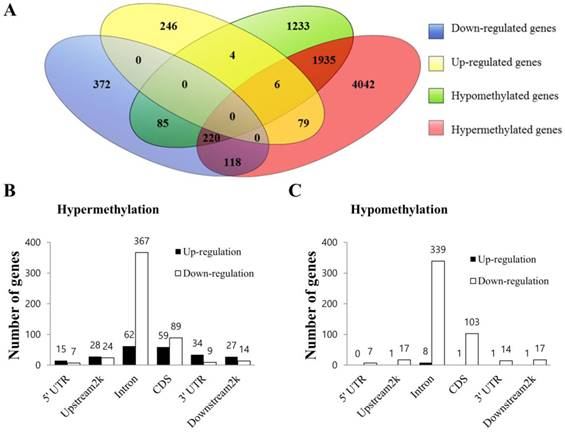
\includegraphics[width=0.8\textwidth]{journal-of-cancer_sample-result}}
	\caption{یک نمونه نمودار خلاصه برای نمایش نوآوری در نتایج
		%\cite{kim2016integrated}
	}
	\label{fig:sampleDiagram}
\end{figure}\\
طبیعتاً به صلاحدید نگارنده، شکل‌ها و نمودار‌ها می توانند در بخش های مختلف، خصوصا فصل
\ref{chap:results}
مورد استفاده قرار گیرند.

\subsection{تعریف واژه‌ها (اختیاری)}
در این قسمت محقق باید واژه‌هایی را که ممکن است برای خواننده آشنا نباشد، تعریف کند.

\subsection{خلاصه فصل‌ها}
در آخرین قسمتِ فصل اول پایان‌نامه، خلاصه‌ای اشاره‌وار از فصل‌های آتی آورده می‌شود تا خواننده بتواند تصویری واضح از دیگر قسمت‌های پایان‌نامه در ذهن خود ترسیم کند.

\section{جمع‌بندی}
در این فصل به دو مقولهٔ نحوه استفاده از قالب \پ دانشگاه تهران و نیز ویژگی‌هایی که محتویات فصل اول پایان‌نامه (یعنی مقدمه) باید داشته باشند، پرداخته شد. با توجه به اینکه این راهنما نحوه استفاده از قالب را شرح داده، ملزومات محتوایی هر فصل پایان‌نامه را توضیح می‌دهد و در پیوست‌ها نیز نحوهٔ کار با لاتک را یادآوری خواهد کرد، بنابراین مطالعهٔ کامل آن مقداری وقت شما را خواهد گرفت؛ اما مطمئن باشید از اتلاف وقت شما در ادامه کارتان تا حد زیادی جلوگیری خواهد کرد. در نوشتن متن حاضر سعی شده است علاوه بر ایجاد یک قالب لاتک برای پایان‌نامه‌های دانشگاه تهران، نکات محتوایی هر فصل نیز گوشزد گردد. طبیعتاً برای نگارش پایان‌نامهٔ خود می‌بایست مطالب تمام فصل‌ها را خودتان بازنویسی کنید.

در ادامهٔ این راهنما، تنها فصل‌هایی که یک پایان‌نامه باید داشته باشد و نیز خصوصیات یا ساختاری که محتویات هر فصل باید از آنها برخوردار باشد%
\footnote{از روی فایل «تمپلیت نگارش و تدوین پایان‌نامه \cite{UTThesisGuide}»}،
آورده می‌شوند. نهایتاً  در پیوست‌ها، مطالبی در باب یادآوری دستورات لاتک، نحوه نوشتن فرمول‌ها، تعاریف، قضایا، مثال‌ها، درج تصاویر، نمودارها، جداول و الگوریتم‌ها و نیز مدیریت مراجع، آمده است.

همچنین توصیه اکید دارم که رفع خطاهایی که احتمالاً با آنها مواجه می‌شوید را به آخر موکول نفرمایید و به محض برخورد با خطا، آن را اشکال‌زدایی و برطرف نمائید.!
و
\verb!% !TeX root=../main.tex
\setcounter{topnumber}{5}      % Increase number of floats at the top of the page
\setcounter{totalnumber}{5}    % Increase total number of floats on a page
\renewcommand{\floatpagefraction}{.8}  % Allow more of the page to be taken up by floats

\chapter{مروری بر مطالعات انجام شده}
%\thispagestyle{empty} 
\section{مقدمه}
در این فصل، پژوهش‌های پیشین در زمینه‌ی موتورهای مسطح مبتنی بر شناوری مغناطیسی (MLPM) با تمرکز بر ویژگی‌های اساسی آنان که به طور کلی در بخش‌های زیر دسته‌بندی شده‌اند، مورد بررسی قرار می‌گیرند. 
\begin{itemize}
	\item
		\textit{معماری دستگاه}:
بررسی انواع معماری‌های موجود برای MLPM و تأثیر آن‌ها بر عملکرد کلی سیستم.
	\item
		\textit{ساختار آهنرباهای دائمی و الکتریکی}:
مرور انواع آهنرباهای الکتریکی و چینش‌های مختلف آهنربا‌های دائمی و نقش آن‌ها در بهینه‌سازی عملکرد سیستم.
	\item
		\textit{طراحی کنترلر}:
معرفی روش‌های کنترل کلاسیک و مدرن برای این سیستم‌ها و چگونگی بهبود پایداری و دقت حرکت.
	\item
		\textit{روش‌های شناسایی سیستم و مدل‌سازی دینامیکی}:
تحلیل روش‌های شناسایی و تخمین مدل‌های دینامیکی سیستم برای شبیه‌سازی و بهینه‌سازی عملکرد.
\end{itemize}
در بخش‌های بعد، پژوهش‌های انجام‌شده بر اساس این ویژگی‌ها ارزیابی شده و مزایا و معایب هر روش مورد بررسی قرار می‌گیرد.

\section{معماری دستگاه‌های MLPM}
سیستم‌های شناوری مغناطیسی به دلیل ماهیت ناپایدارشان بدون استفاده از حلقه‌های کنترلی نمی‌توانند پایداری لازم را فراهم کنند. به همین دلیل، در تمامی ساختارهای پیشنهادی، از سیم‌پیچ‌های الکتریکی برای تولید میدان مغناطیسی با شدت کنترل ‌شده استفاده می‌شود. این سیم‌پیچ‌ها وظیفه دارند تا موقعیت جسم معلق را پایدار کرده و آن را در حالت مطلوب نگه ‌دارند.

در طراحی موتورهای مسطح، که از دو بخش ثابت
\LTRfootnote{Stator}
 و متحرک
\LTRfootnote{Mover}
تشکیل شده‌اند، امکان تغییر در طراحی و محل قرارگیری آهنرباهای الکتریکی و دائمی وجود دارد. نیروی مغناطیسی وارد بر بخش متحرک می‌تواند به‌صورت جاذبه‌ای از بالا یا دافعه‌ای از پایین اعمال شود. با این حال، در موتورهای مسطح به دلیل لزوم کم بودن فاصله میان سیم‌پیچ‌ها و اجسام معلق، اعمال نیروی جاذبه‌ای از بالا امکان‌پذیر نیست. به همین دلیل، در تمامی طراحی‌ها، نیروی مغناطیسی دافعه‌ای از سمت پایین به بخش متحرک وارد می‌شود که امکان جابه‌جایی اجسامی که بر روی آنها قرار می‌گیرند را فراهم می‌کند.

با توجه به این موارد، دو طراحی کلی برای ساخت دستگاه‌های MLPM ارائه می‌شود که در ادامه بررسی می‌‌شوند.
\subsection{سیم‌پیچ‌های متحرک و آهنرباهای ثابت}

در این معماری، بخش استاتور از مجموعه‌ای آهنربای ثابت تشکیل شده که میدان مغناطیسی پایدار در محیط اطراف خود ایجاد می‌کنند. بخش متحرک دستگاه شامل سیم‌پیچ‌هایی است که با عبور جریان الکتریکی از آن‌ها، میدان مغناطیسی متغیری تولید می‌گردد. این جریان به گونه‌ای تنظیم می‌شود که نیروی وارد بر آهنرباهای دائمی به‌دقت کنترل شود. طبق قانون سوم نیوتن، نیروهای وارد بر سیم‌پیچ‌ها و آهنرباهای دائمی به‌عنوان عمل و عکس‌العمل رفتار می‌کنند؛ به این ترتیب، نیرویی که به آهنرباها اعمال می‌شود، باعث ایجاد نیرویی برابر و در جهت مخالف بر سیم‌پیچ‌ها خواهد شد.

در پژوهش 
\cite{RN49}
، از ساختاری با سیم‌پیچ‌های چندلایه متعامد در بخش متحرک استفاده شده است. لایه اول سیم‌پیچ‌ها نیرویی را در راستاهای x و z ایجاد می‌کند، در حالی که لایه دوم نیرو را در راستاهای y و z اعمال می‌کند. این جداسازی نیروها به بهبود کنترل سیستم کمک می‌کند. علاوه بر این، به دلیل تفاوت فاصله میان لایه‌ها و استاتور، نیروهای تولیدشده توسط هر لایه متفاوت خواهند بود. راهکار ارائه‌شده برای این چالش، افزایش ضخامت لایه‌های دورتر از استاتور است. با این حال، برای جلوگیری از مشکلات ناشی از تفاوت ضخامت لایه‌ها، ساختاری سه‌لایه طراحی شده که ضمن افزایش نیروی تولیدی، ضخامت یکنواختی را در تمامی راستاها فراهم می‌نماید. در شکل 
\ref{fig:Multilayer_Mover_Coil}
ساختار این دستگاه نمایش داده شده است.

در پژوهش 
\cite{RN38}
، بخش متحرک از یک لایه سیم‌پیچ با چینش متعامد تشکیل شده که قابلیت اعمال نیرو در سه راستا را فراهم می‌سازد. در ادامه، پژوهش
\cite{RN14}
 روشی تحلیلی برای بهینه‌سازی ضخامت این سیم‌پیچ‌ها ارائه کرده است که با در نظر گرفتن معیارهای مختلف، به بهبود عملکرد سیستم می‌پردازد. شکل 
\ref{fig:Single_layer_Mover_Coil}
 این ساختار را نمایش داده است.

\begin{figure}[ht]
\centering 
\subfloat[استفاده از سیم‌پیچ‌های چندلایه
\cite{RN49}]
{ \label{fig:Multilayer_Mover_Coil}
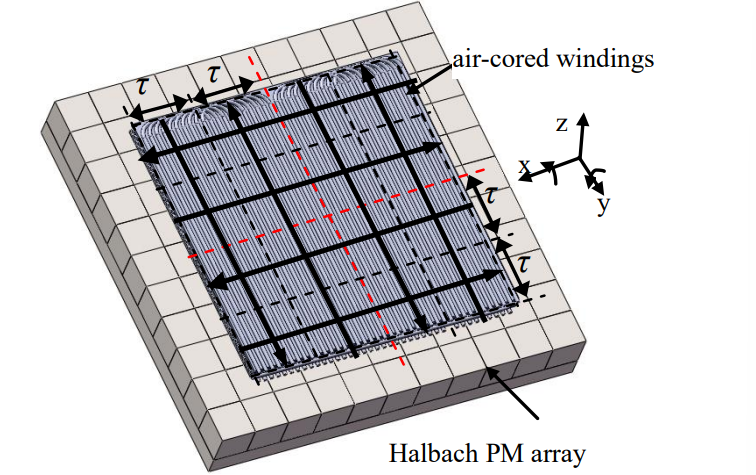
\includegraphics[width=0.5\textwidth]{Multilayer_Mover_Coil}}
%\hspace{2mm}
\subfloat[استفاده از سیم‌پیچ‌های یک لایه متعامد
\cite{RN14}]
{ \label{fig:Single_layer_Mover_Coil}
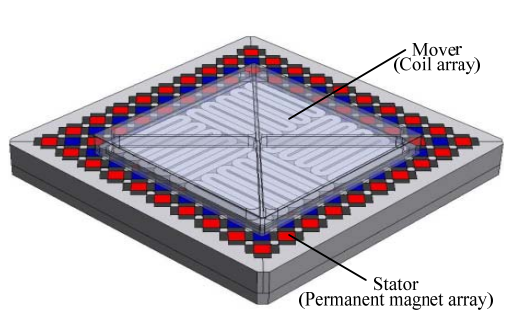
\includegraphics[width=0.5\textwidth]{Single_layer_Mover_Coil}}%
\caption{ساختار سیستم‌های MLPM با سیم‌پیچ‌های متحرک و آهنربای ثابت}
\label{fig:Moveing_Coil} %% label for entire figure
\end{figure}

با وجود اینکه این معماری امکان دستیابی به شناوری پایدار و حرکت با شش درجه آزادی را فراهم می‌کند، اما در کاربردهای عملی با محدودیت‌هایی مواجه است که بر عملکرد نهایی سیستم تأثیرگذار هستند. نخستین محدودیت، نیاز به تأمین انرژی الکتریکی برای سیم‌پیچ‌ها از طریق سیم‌های فیزیکی است که این امر به‌طور اجتناب‌ناپذیری ارتباط فیزیکی میان جسم متحرک و محیط اطراف را برقرار می‌سازد، در نتیجه حرکت آزادانه کامل جسم متحرک محدود می‌شود. دومین محدودیت، چالش خنک‌کاری سیم‌پیچ‌ها است که به دلیل ماهیت متحرک و معلق بودن آن‌ها، اجرای یک سیستم خنک‌کننده کارآمد دشوار خواهد بود. این مشکلات، نیاز به ارائه معماری جدیدی را آشکار می‌کند که بتواند این چالش‌ها را برطرف سازد.

\subsection{‌آهنرباهای متحرک و سیم‌پیچ‌های ثابت}

معماری دیگری که برای طراحی دستگاه‌های MLPM ارائه شده است، شامل قرار دادن سیم‌پیچ‌ها در بخش استاتور و استفاده از آهنرباهای دائمی در بخش متحرک می‌باشد. این ساختار نوین که در بسیاری از پژوهش‌ها مورد استفاده قرار گرفته، مشکلات معماری‌های پیشین مانند محدودیت جابه‌جایی متحرک ناشی از اتصالات فیزیکی و چالش‌های خنک‌کاری سیم‌پیچ‌ها را برطرف کرده و منجر به بهبود عملکرد کلی سیستم شده است.

در پژوهش 
\cite{RN7}
 استاتوری با چینش سیم‌پیچ‌ها مطابق با الگوی شاه‌ماهی
\LTRfootnote{Herringbone pattern}
 طراحی و پیاده‌سازی شده است. این طراحی امکان اعمال نیروی مغناطیسی به دو آهنربای دیسکی تعبیه‌شده در بخش متحرک را فراهم کرده است که دقتی در حدود 1 درجه در زوایای حرکت و 1 میلی‌متر در موقعیت متحرک به دست آورده است
\cite{RN7}
. در ادامه این پژوهش، ساختاری جدید برای بخش متحرک ارائه شده که شامل 6 آهنربای دیسکی با چینش کروی و فواصل ثابت می‌باشد. این طراحی توانسته است چرخش آزادانه متحرک را حول سه محور ممکن سازد 
\cite{RN39}.
شکل (
\ref{fig:Moving_Magnet_1})
همچنین در پژوهش 
\cite{RN62}
 نیز از این چینش سیم‌پیچ‌ها استفاده شده و مطابق با شبیه‌سازی‌های ارائه شده، مزیت آنان در ایجاد میدان مغناطیسی یکنواخت‌تر در نواحی کناری سیم‌پیچ‌ها نمایش داده شده است.

استفاده از سیم‌پیچ‌های سه‌فاز به‌جای تغذیه با جریان مستقیم، رویکردی است که در پژوهش 
\cite{RN24}
معرفی و اجرا شده است. در این ساختار، چهار آرایه از سیم‌پیچ‌های سه‌فاز، همان‌طور که در 
شکل (
\ref{fig:Moving_Magnet_2})
 نشان داده شده است، به‌گونه‌ای طراحی شده‌اند که نیروی مغناطیسی لازم را تولید کنند.

به ‌منظور کاهش هزینه‌ی محاسباتی در جابه‌جایی‌های طولانی، پژوهش 
\cite{RN32}
 ساختاری را ارائه کرده است که از دو مجموعه سیم‌پیچ‌ سه‌فاز و تک‌فاز تشکیل شده است. در این طراحی، کنترل حرکت در مسافت‌های طولانی توسط سیم‌پیچ‌های سه‌فاز انجام می‌پذیرد، در حالی که برای تنظیم دقیق موقعیت متحرک در صفحه، از سیم‌پیچ‌های تک‌فاز بهره برده می‌شود.
شکل (
\ref{fig:Moving_Magnet_3})

استفاده از سیم‌پیچ‌های ماژولار در طراحی استاتورهایی با چینش دوبعدی، رویکردی است که در دستگاه‌های MagTable و MagFloor از دانشگاه واترلو پیاده‌سازی شده است
\cite{RN8,RN30,RN10}
 در این طراحی، ماژول‌هایی از سیم‌پیچ‌های با سطح مقطع مربع به‌گونه‌ای طراحی شده‌اند که با قرار گرفتن در کنار یکدیگر، فضای کاری نامحدودی برای جابه‌جایی متحرک فراهم می‌کنند.(شکل
\ref{fig:Moving_Magnet_4})
 همچنین، پژوهش
\cite{RN8}
 نشان داده است که آهنرباهای با سطح مقطع مربع، در مقایسه با سیم‌پیچ‌های دایروی با جریان الکتریکی مشابه، می‌توانند شدت میدان مغناطیسی بیشتری ایجاد کنند، که این مزیت عملکرد کلی سیستم را بهبود می‌بخشد.

\begin{figure}[ht]
\centering 
\subfloat[الگوی شاه‌ماهی سیم‌پیچ‌ها
\cite{RN39}]
{ \label{fig:Moving_Magnet_1}
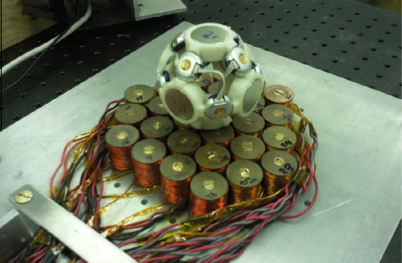
\includegraphics[width=0.45\textwidth]{Moving_Magnet_1}}
\hspace{2mm}
\subfloat[سیم‌پیچ‌های سه فاز
\cite{RN24}]
{ \label{fig:Moving_Magnet_2}
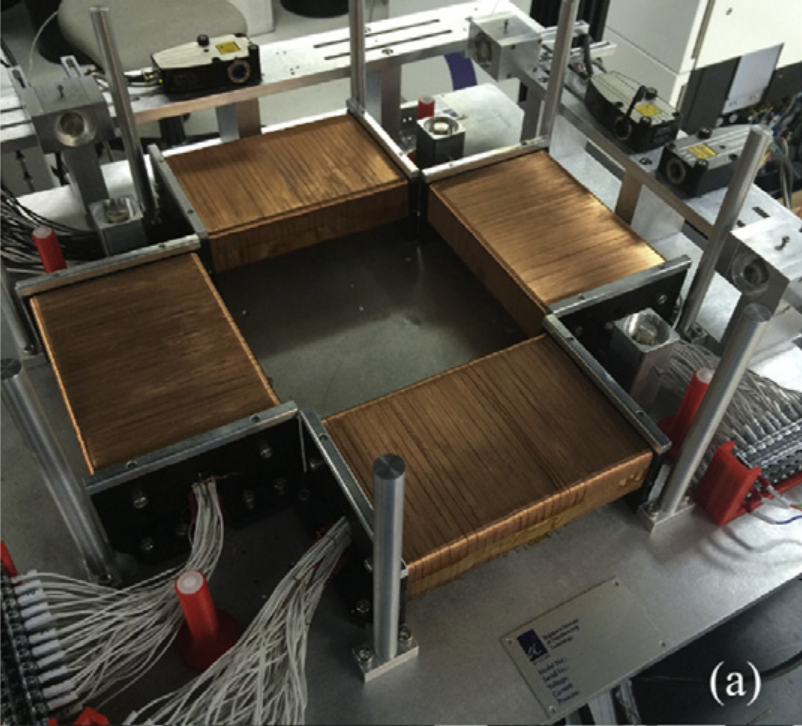
\includegraphics[width=0.45\textwidth]{Moving_Magnet_2}}
\\ % Newline to wrap the figures to the next row
\subfloat[ساختار دوگانه سیم‌پیچ‌ها
\cite{RN32}]
{ \label{fig:Moving_Magnet_3}
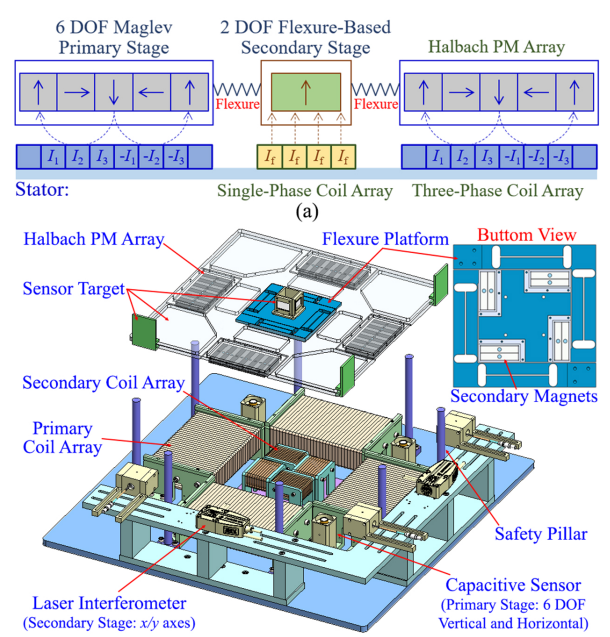
\includegraphics[width=0.45\textwidth]{Moving_Magnet_3}}
\hspace{2mm}
\subfloat[ساختار ماژولار سیم‌پیچ‌ها
\cite{RN10}]
{ \label{fig:Moving_Magnet_4}
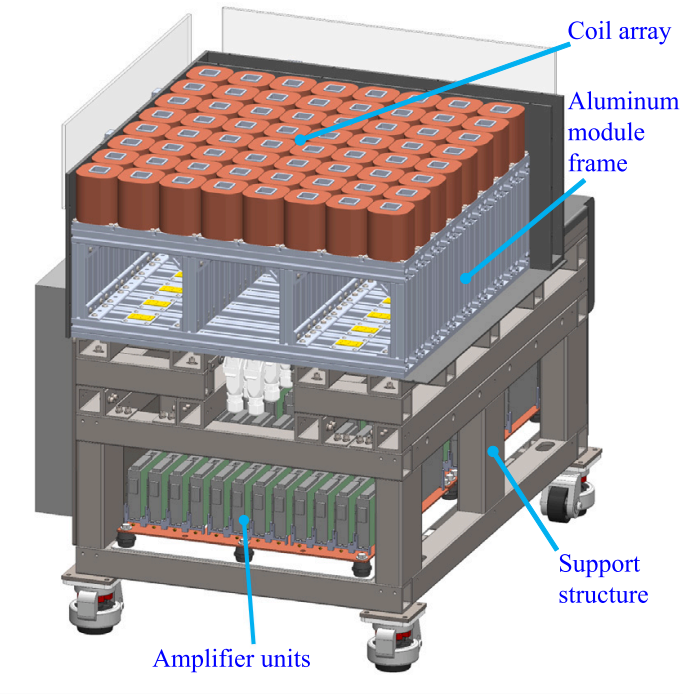
\includegraphics[width=0.45\textwidth]{Moving_Magnet_4}}
\label{fig:Moveing_Magnet} %% label for entire figure
\caption{ساختارهای آهنرباهای متحرک و سیم‌پیچ‌های ثابت}
\end{figure}








\section{ساختار آهنرباهای دائمی}

همان‌طور که در بخش قبل اشاره شد، میدان مغناطیسی کنترل‌شده توسط آهنرباهای الکتریکی ایجاد می‌شود و بر اثر تعامل این میدان متغیر با میدان ثابت آهنرباهای دائمی، نیرویی بر بخش متحرک دستگاه وارد می‌شود که حرکت آن را در راستاهای مختلف ممکن می‌سازد. بنابراین، طراحی بهینه آهنرباهای دائمی، به‌ویژه برای تولید میدان مغناطیسی قوی‌تر با کمترین وزن، در بهبود کارایی دستگاه نقش کلیدی دارد. در این بخش، طراحی‌های مختلف آهنرباهای دائمی که در پژوهش‌های پیشین ارائه شده‌اند، با تمرکز بر بهینه‌سازی این ویژگی‌ها بررسی می‌شوند.
\subsection{استفاده از آهنرباهای دیسکی}

استفاده از آهنرباهای دیسکی رویکردی ساده و مؤثر برای ایجاد میدان مغناطیسی دائمی محسوب می‌شود. با انتخاب موادی با خاصیت مغناطیسی بالا، مانند آهنرباهای نئودیمیومی، می‌توان به شدت میدان مغناطیسی مطلوب دست یافت. به عنوان نمونه، در پژوهش 
\cite{RN7}
 از دو آهنربای دیسکی جهت تأمین میدان مغناطیسی ثابت استفاده شده است. همچنین در پژوهش 
\cite{RN39}
 با به‌کارگیری ۶ آهنربای دیسکی، امکان چرخش آزادانه حول سه محور فراهم شده است.(شکل
\ref{fig:Disk_Magnet_1})
 در پژوهش 
\cite{RN8}
 نیز از ترکیب‌های متفاوتی از آهنرباهای دیسکی برای بخش متحرک دستگاه استفاده شده است، که این ترکیب‌ها شامل تغییر اندازه‌ی یک آهنربا و استفاده از سه آهنربای دیسکی است. سیستم شناوری مغناطیسی با پنج درجه آزادی که تنها از یک آهنربای دیسکی تشکیل شده است، در پژوهش 
\cite{RN62}
 به عنوان نمونه‌ای موفق از این رویکرد معرفی شده است. این طراحی، با وجود سادگی معماری، توانسته نتایج رضایت‌بخشی را از نظر عملکرد ارائه دهد و نشان می‌دهد که استفاده از آهنربای دیسکی، علاوه بر سادگی، می‌تواند در کاربردهای مختلف به‌ویژه در سیستم‌های با نیاز به دقت بالا و چند درجه آزادی، کارآمد باشد. شکل((
\ref{fig:Disk_Magnet_2})


\begin{figure}[ht]
\centering 
\subfloat[دو آهنربای دیسکی
\cite{RN7}]
{ \label{fig:Disk_Magnet_1}
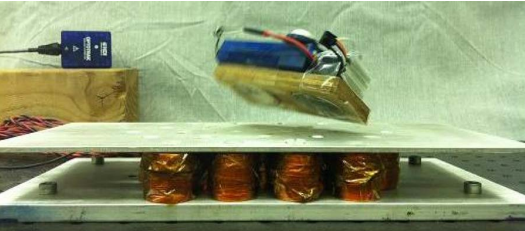
\includegraphics[width=0.5\textwidth]{Disk_Magnet_1}}
%\hspace{2mm}
\subfloat[یک آهنربای دیسکی
\cite{RN62}]
{ \label{fig:Disk_Magnet_2}
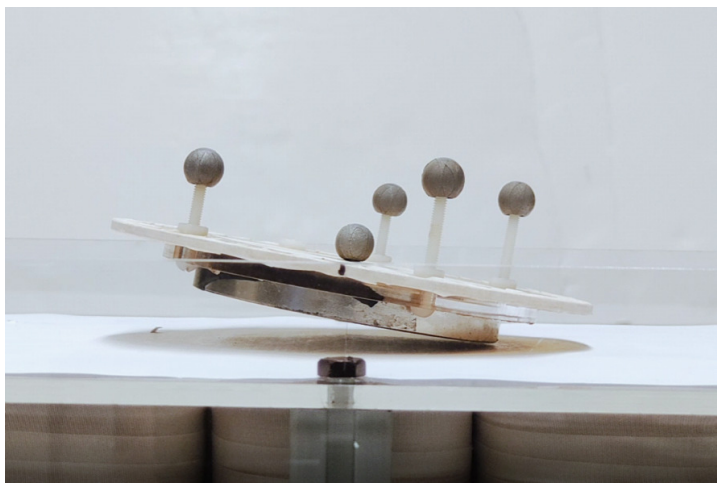
\includegraphics[width=0.5\textwidth]{Disk_Magnet_2}}%
\caption{استفاده از آهنربای دیسکی در طراحی متحرک}
\label{fig:Disk_Magnet} %% label for entire figure
\end{figure}



\subsection{آرایه‌ی هالباخ یک بعدی}

آرایه‌ی هالباخ
\LTRfootnote{Halbach Array}
 به‌عنوان چینشی از آهنرباهای دائمی تعریف می‌شود که در آن جهت مغناطیس‌شوندگی هر آهنربا با آهنربای مجاور خود ۹۰ درجه تفاوت دارد. این آرایه به‌طور خاص قادر است میدان مغناطیسی در یک سوی آرایه را خنثی کرده و در سوی دیگر میدان را به میزان تقریبی 1.4 برابر افزایش دهد.
مزیت این ساختار در طراحی سیستم‌های MLPM، توانایی آن در تولید شدت میدان مغناطیسی بیشتر است. به‌همین‌دلیل، این چینش در بسیاری از پژوهش‌ها مورد استفاده قرار گرفته است.
با این حال، استفاده از تنها یک آرایه‌ی یک‌بعدی هالباخ به‌تنهایی نمی‌تواند نیرویی در دو راستای افقی ایجاد کند. لذا معمولاً از تعداد بیشتری از این آرایه‌ها در ساختار متحرک استفاده می‌شود. به‌عنوان مثال، در پژوهش‌های 
\cite{RN24,RN27}
 از چهار آرایه‌ی هالباخ یک‌بعدی در بخش متحرک استفاده شده است که هر یک از این آرایه‌ها قادر به ایجاد نیرویی در یکی از راستاهای افقی و عمودی هستند.
در پژوهش 
\cite{RN39}
، مشابه آنچه که در بخش استاتور پیاده‌سازی شده بود، از ساختار دوگانه‌ای در بخش متحرک بهره‌برداری شده است، به‌گونه‌ای که دو مجموعه چهارگانه از آرایه‌های هالباخ در معماری این بخش به‌کار رفته‌اند.

\begin{figure}[ht]
\centering 
\subfloat[آرایه‌ی هالباخ
\cite{RN16}]
{ \label{fig:halbach1D}
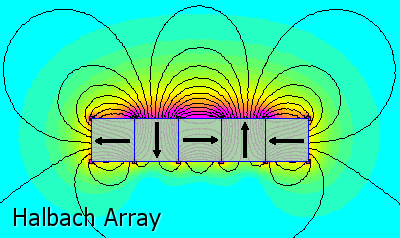
\includegraphics[width=0.5\textwidth]{halbach1D}}
%\hspace{2mm}
\subfloat[4 آرایه‌ی یک بعدی هالباخ
\cite{RN39}]
{ \label{fig:4_halbach1D_array}
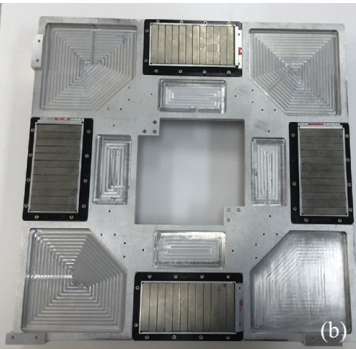
\includegraphics[width=0.5\textwidth]{4_halbach1D_array}}%
\caption{آرایه هالباخ یک‌بعدی}
\label{fig:halbach1D} %% label for entire figure
\end{figure}

\subsection{آرایه هالباخ دوبعدی}

برای رفع محدودیت‌های آرایه‌ی هالباخ یک‌بعدی که تنها در یک راستا نیرو ایجاد می‌کند، ساختار جدیدی از آرایه‌ی دوبعدی ارائه شده است. این آرایه قادر است میدان مغناطیسی را در یک طرف صفحه حذف و در طرف دیگر تقویت کند. با این ویژگی، استفاده از چندین آرایه برای تأمین میدان مغناطیسی ثابت ضروری نخواهد بود. طراحی آرایه‌ی دوبعدی در بسیاری از پژوهش‌ها برای بخش‌های متحرک یا استاتور سیستم‌های MLPM به کار گرفته شده است.

استفاده از آرایه‌ی هالباخ در پژوهش‌های مختلفی از جمله
\cite{RN10, RN30} 
و
\cite{RN55, RN26} 
نشان‌دهنده‌ی عملکرد بهینه‌ی این معماری در بخش متحرک سیستم‌های MLPM است.(شکل
\ref{fig:halbach2D_2})
 همچنین در پژوهش
\cite{RN14}
 از این آرایه به عنوان بخشی از استاتور دستگاه بهره‌گیری شده است. در 
\cite{RN61}
 ماژول‌هایی برای ساخت این آرایه استفاده شده (شکل
\ref{fig:halbach2D_4})
 و در
\cite{RN49}
 برای تشکیل آرایه از قطعات آهنی در فضای خالی میان آن استفاده شده است؛ اما این رویکرد باعث ایجاد خطا در دقت میدان مغناطیسی شده است. (شکل
\ref{fig:halbach2D_3})
علاوه بر این، در پژوهش
\cite{RN28}
، طراحی جدیدی با آهنرباهایی با میزان مغناطیس‌شوندگی و ارتفاع متفاوت پیشنهاد شده است.
\begin{figure}[ht]
\centering 
\subfloat[آرایه هالباخ دو بعدی و میدان مغناطیسی آن
\cite{RN10}]
{ \label{fig:halbach2D_2}
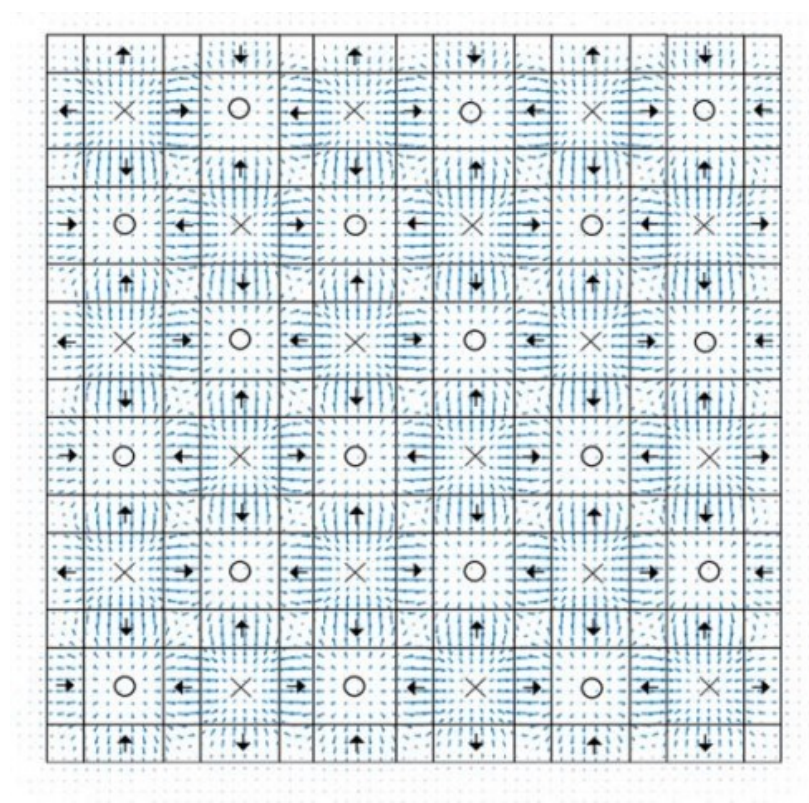
\includegraphics[width=0.45\textwidth]{halbach2D_2}}
\hspace{2mm}
\subfloat[آرایه هالباخ دوبعدی با قطعات آهنی در فضاهای خالی
\cite{RN49}]
{ \label{fig:halbach2D_3}
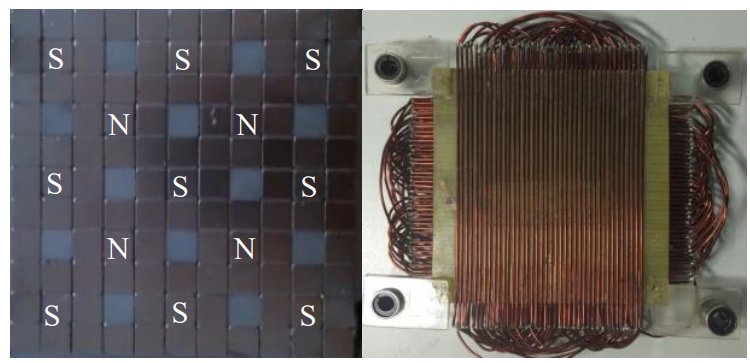
\includegraphics[width=0.45\textwidth]{halbach2D_3}}
\\ % Newline to wrap the figures to the next row
\subfloat[آرایه هالباخ دوبعدی ماژولار
\cite{RN61}]
{ \label{fig:halbach2D_4}
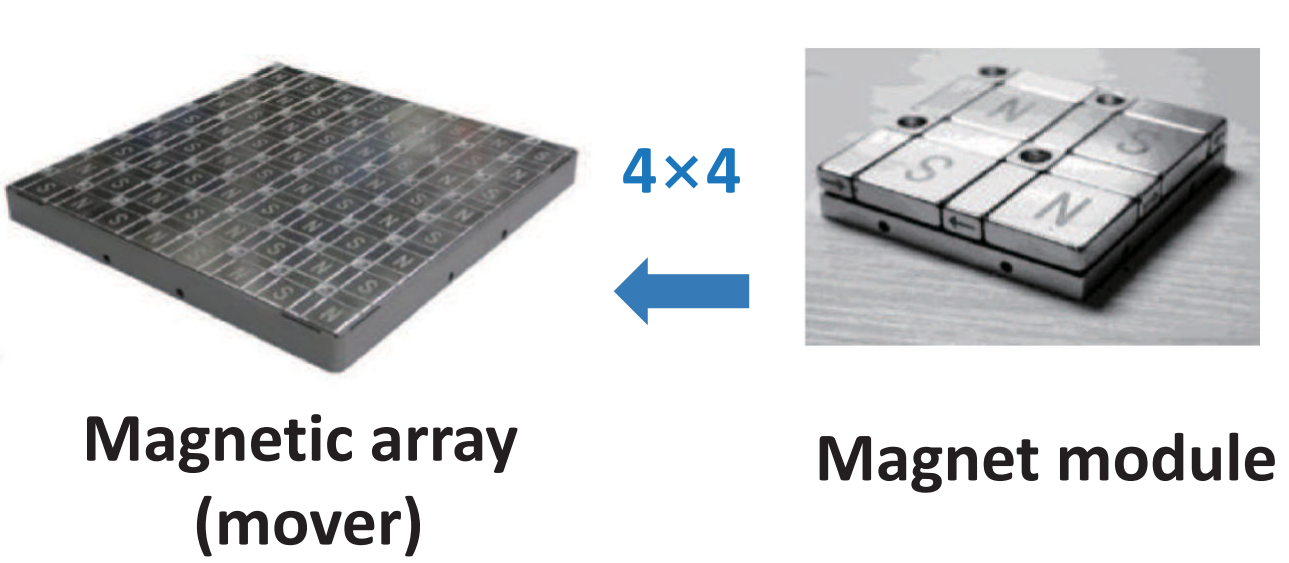
\includegraphics[width=0.45\textwidth]{halbach2D_4}}
\caption{آرایه هالباخ دو‌بعدی}
\label{fig:halbach2D} %% label for entire figure

\end{figure}
\section{طراحی کنترلر}
همان‌طور که پیش‌تر اشاره شد، سیستم‌های شناوری مغناطیسی ذاتاً ناپایدار هستند و برای دستیابی به پایداری، به کنترلری با عملکرد دقیق و خطای کم نیاز است. در پژوهش‌های مختلف، از کنترلرهای گوناگونی برای این سیستم‌ها بهره گرفته شده است؛ از جمله کنترلرهای کلاسیک نظیر PID، کنترلرهای مدرن مانند کنترل مبتنی بر پیش‌بینی مدل (MPC) و همچنین مدل‌های مبتنی بر هوش مصنوعی نظیر شبکه‌های بازگشتی GRU. در این بخش، به بررسی این کنترلرها و مقایسه‌ عملکرد آنها خواهیم پرداخت.
\subsection{کنترلر PID}

کنترل تناسبی-انتگرالی-مشتقی (PID) به عنوان یکی از پرکاربردترین و موثرترین کنترلرهای کلاسیک در سیستم‌های دینامیکی، گزینه‌ای مناسب برای کنترل سیستم‌های MLPM محسوب می‌شود. این کنترلر به دلیل سادگی در پیاده‌سازی، تنظیم دقیق و توانایی تنظیم خروجی سیستم بر اساس خطاهای ورودی، به‌طور گسترده در سیستم‌های مختلف استفاده شده است. برای کنترل سیستم‌های MLPM، به ازای هر درجه آزادی یک کنترلر PID طراحی و پیاده‌سازی می‌شود تا بتواند جریان الکتریکی سیم‌پیچ‌ها را تنظیم کرده و میدان مغناطیسی لازم برای ایجاد و حفظ موقعیت متحرک را تأمین کند.

در پژوهش‌های متعددی از کنترلر PID برای سیستم‌های MLPM بهره گرفته شده است. به عنوان مثال، در 
\cite{RN39,RN24}
از کنترلرهای PID ساده برای کنترل جریان سیم‌پیچ‌ها استفاده شده که وظیفه تنظیم میدان مغناطیسی و در نتیجه، کنترل موقعیت جسم متحرک را بر عهده دارند. علاوه بر این، در پژوهش
\cite{RN32}
، از دو کنترلر PID در یک ساختار دوگانه استفاده شده است. کنترلر اول برای جابه‌جایی‌های بلند و در مسافت‌های طولانی به کار رفته و جریان سیم‌پیچ‌های اصلی را تنظیم می‌کند، در حالی که کنترلر دوم برای حرکات دقیق کوتاه‌برد طراحی شده و کنترل جریان سیم‌پیچ‌های ثانویه را بر عهده دارد. این روش باعث بهینه‌سازی کنترل دقیق و بهبود دقت در حرکات کوتاه‌برد و جابه‌جایی‌های سریع می‌شود.
همچنین در سیستم MagTable، برای کنترل دقیق موقعیت آهنرباهای دائمی، از شش کنترلر PID به‌صورت همزمان استفاده شده است تا نیروی متوازن برای پایدارسازی موقعیت متحرک در چندین جهت فراهم شود 
\cite{RN8}
. این نوع طراحی و استفاده از کنترلرهای PID نشان می‌دهد که علی‌رغم محدودیت‌های موجود در کنترلرهای کلاسیک، این روش همچنان در بسیاری از سیستم‌های مغناطیسی پیچیده مانند MLPM کارایی بالایی دارد.

\begin{figure}[ht]
\centering{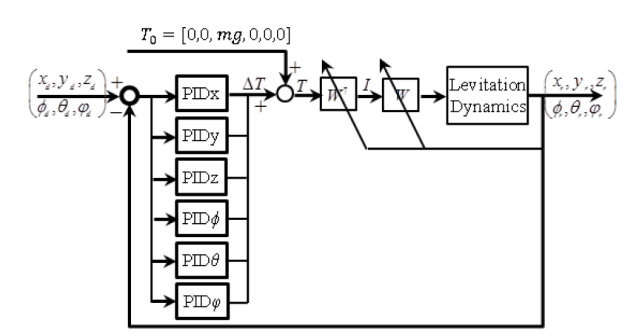
\includegraphics[width=0.5\textwidth]{PID_1}}
\caption{کنترلر PID با 6 درجه آزادی
\cite{RN8}}
\label{fig:PID}
\end{figure}


\subsection{کنترلر مبتنی بر پیش‌بینی مدل MPC}
برای کنترل سیستم‌های MLPM اگر مدل سیستم به روش‌های تحلیلی و یا عددی به دست آمده و تخمین زده شده باشد، می‌توان از این مدل‌ها برای طراحی کنترلرهای پیشرفته‌تر با هدف پیش‌بینی رفتار سیستم و استفاده از آن به صورت پیش‌خور در حلقه‌ی کنترلی استفاده کرد. روش‌های تخمین مدل این سیستم‌ها در بخش‌های بعد مورد بررسی قرار می‌گیرد. در این بخش، کنترلرهای ارائه شده در پژوهش‌های دیگر ارائه می‌شود.
به دست آوردن معادلات دینامیکی سیستم و استفاده از آنها در پیش‌بینی روشی تحلیلی است که در 
\cite{RN55}
 استفاده شده است و مدل کنترلی متشکل از بلوک‌های پس‌خور و پیش‌خور برای کنترل موقعیت آهنربا طراحی شده است. همچنین در 
\cite{RN62}
 از یک جدول جستجو برای تعیین رفتار سیستم در نقاط مختلف فضا استفاده شده است که این جدول به عنوان پیش‌خور به مدل کنترلی داده می‌شود. در ادامه‌ی این پژوهش، با استفاده از روش‌های شناسایی سیستم، مدلی تقریبی برای رفتار سیستم در نظر گرفته شده است و با استفاده از این مدل برای پیش‌بینی رفتار سیستم‌ مدل MPC پیاده‌سازی شده است. پژوهش 
\cite{RN30}
 با تمرکز بر ارائه‌ی یک مدل پیش‌بین، با استفاده از معادلات دینامیکی سیستم و همچنین روش‌پیش‌بینی حالت بی‌تاخیر، رفتار آینده‌ی سیستم را محاسبه می‌کند.
\begin{figure}[ht]
\centering 
\subfloat[\cite{RN55}]{
    \label{fig:MPC_1}
    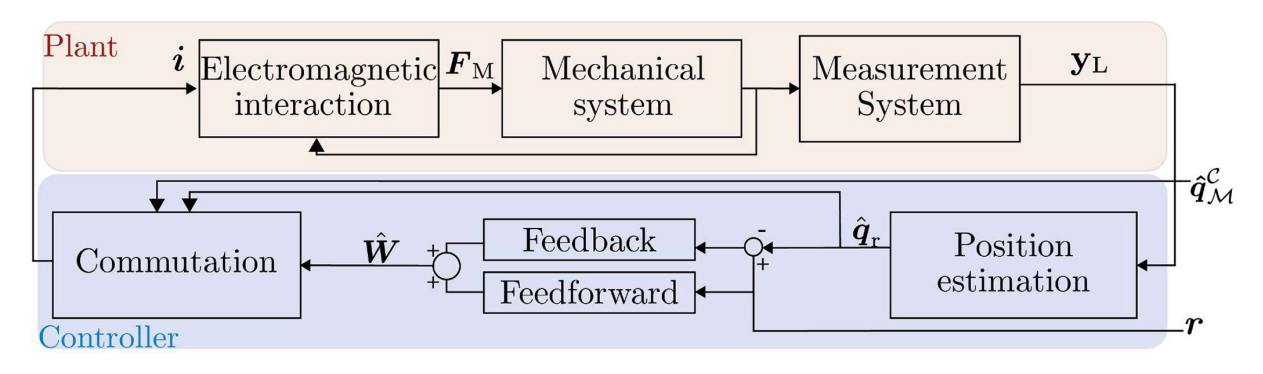
\includegraphics[width=0.45\textwidth]{MPC_1}}
%\hspace{2mm}
\subfloat[\cite{RN62}]{
    \label{fig:MPC_2}
    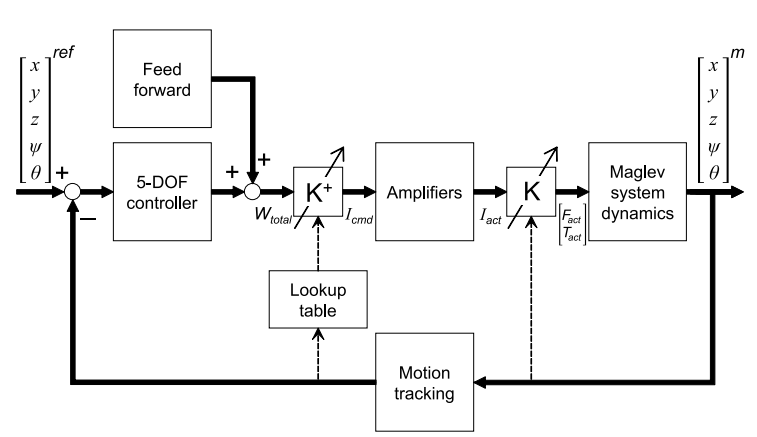
\includegraphics[width=0.45\textwidth]{MPC_2}}
\\ % Newline to wrap the figures to the next row
\subfloat[\cite{RN61}]{
    \label{fig:MPC_3}
    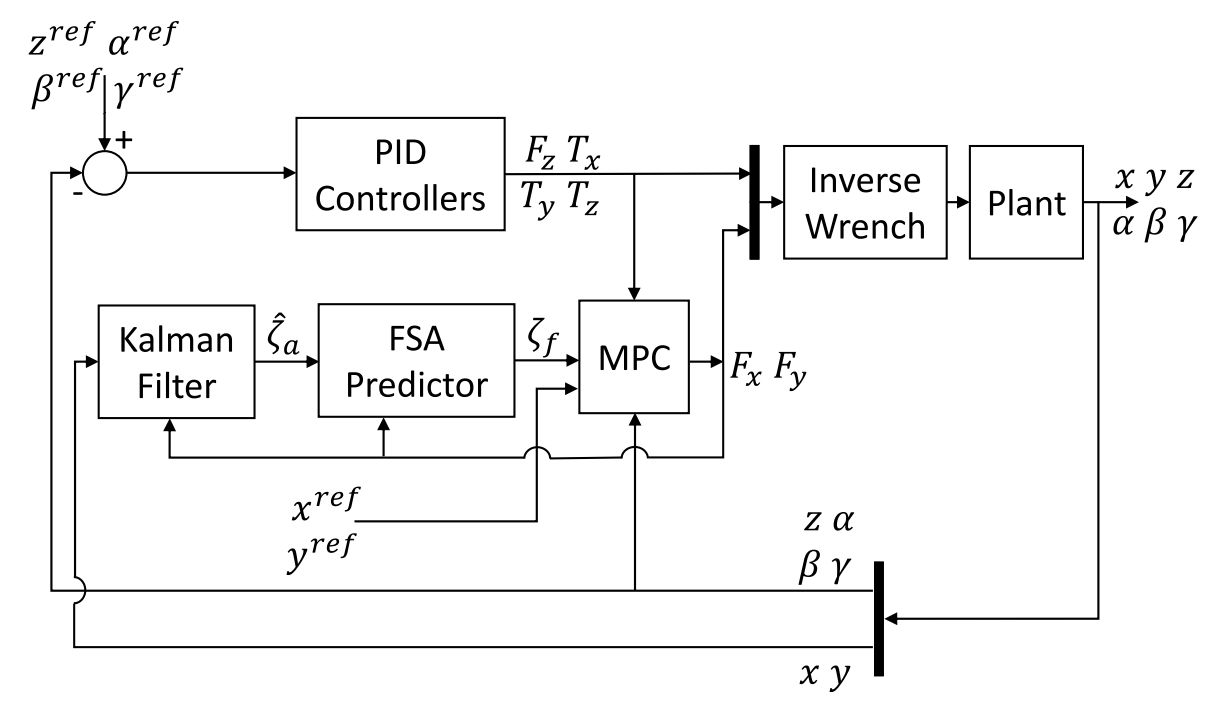
\includegraphics[width=0.45\textwidth]{MPC_3}}
\subfloat[\cite{RN61}]{
    \label{fig:MPC_4}
    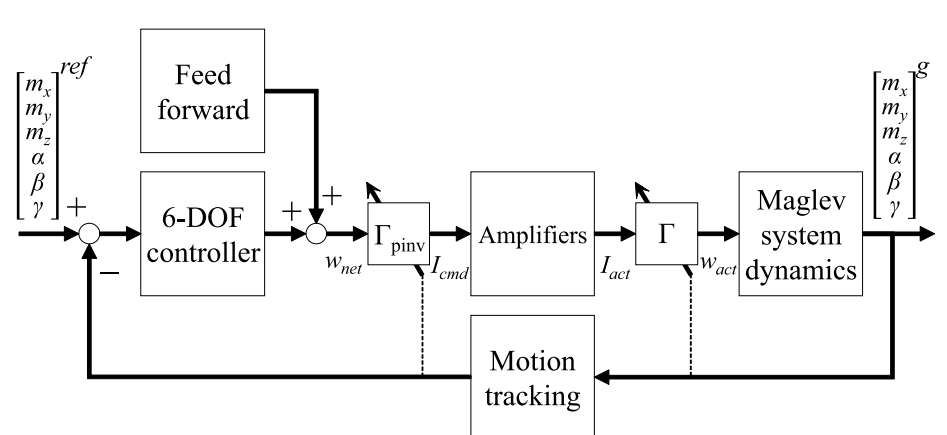
\includegraphics[width=0.45\textwidth]{MPC_4}}
\caption{کنترلر MPC}
\label{fig:MPC} %% label for entire figure
\end{figure}

\FloatBarrier

\subsection{کنترلر مبتنی بر هوش مصنوعی}

یکی از روش‌های نوین برای پیش‌بینی رفتار سیستم‌های پیچیده مانند MLPM، استفاده از مدل‌های هوش مصنوعی به‌ویژه شبکه‌های عصبی بازگشتی (RNN) است. این مدل‌ها با یادگیری دینامیک سیستم و ارتباط بین ورودی‌ها و خروجی‌ها، می‌توانند به‌طور مؤثری رفتار سیستم را در شرایط مختلف پیش‌بینی کنند. در این راستا، پژوهش
\cite{RN61}
از یک مدل بازگشتی GRU 
\LTRfootnote{Gated Recurrent Unit}
 استفاده کرده است. این مدل بر اساس داده‌های جمع‌آوری‌شده از عملکرد دستگاه MLPM آموزش دیده و توانسته است با دقت بالا تغییرات دینامیکی سیستم و پاسخ آن به ورودی‌های گوناگون را پیش‌بینی کند. استفاده از GRU به دلیل توانایی آن در مدل‌سازی وابستگی‌های زمانی و در نظر گرفتن اطلاعات قبلی برای پیش‌بینی‌های دقیق‌تر، رویکردی مناسب در این پژوهش بوده است.(شکل 
\ref{fig:GRU}

\begin{figure}[ht]
\centering
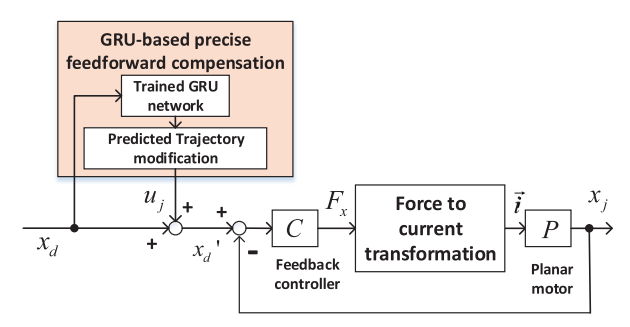
\includegraphics[width=0.5\textwidth]{GRU_1}
\caption{کنترلر پیش‌خور GRU \cite{RN61}}
\label{fig:GRU}
\end{figure}

\section{مدل‌سازی و تخمین سیستم}
در روش بار نقطه‌ای برای تحلیل میدان مغناطیسی، فرض می‌شود که توزیع بار مغناطیسی در یک حجم به‌صورت متمرکز در هشت نقطه در گوشه‌های آن حجم قرار گرفته است. با این فرض، اثر مغناطیسی این جسم می‌تواند به‌صورت مجموع آثار هر یک از بارهای نقطه‌ای محاسبه شود. این رویکرد امکان محاسبه‌ی دقیق شدت میدان مغناطیسی و نیروی وارد بر یک جسم خارجی را فراهم می‌آورد. از طریق محاسبه‌ی میدان‌های ناشی از هر بار نقطه‌ای و جمع آنها، میدان مغناطیسی کل حاصل می‌شود و به این ترتیب، شدت میدان مغناطیسی ناشی از آهنربای دائمی به کمک این روش به‌طور دقیق محاسبه می‌گردد. در ادامه، معادلات مربوط به محاسبه‌ی شدت میدان مغناطیسی ارائه شده‌اند.
\subsection{مدل بار مغناطیسی سطحی}
در این مدل، فرض بر این است که بار مغناطیسی در یک المان حجم سه‌بعدی به‌صورت توزیعی از بارهای مغناطیسی با چگالی بار J بر روی دو صفحه‌ی موازی قرار گرفته است. با استفاده از این فرض، میدان مغناطیسی ایجادشده توسط این حجم به‌صورت میدان حاصل از توزیع بارهای مغناطیسی محاسبه می‌شود. این مدل امکان تحلیل دقیق‌تر رفتار میدان مغناطیسی را فراهم می‌کند. مقایسه نتایج حاصل از این مدل با شبیه‌سازی المان محدود
\LTRfootnote{Finite Element Method (FEM)}
 در پژوهش
\cite{RN44}
نشان داده است که این روش مدل‌سازی برای سیستم‌های MLPM دقت و کارایی بالایی دارد.

\begin{figure}[ht]
\centering
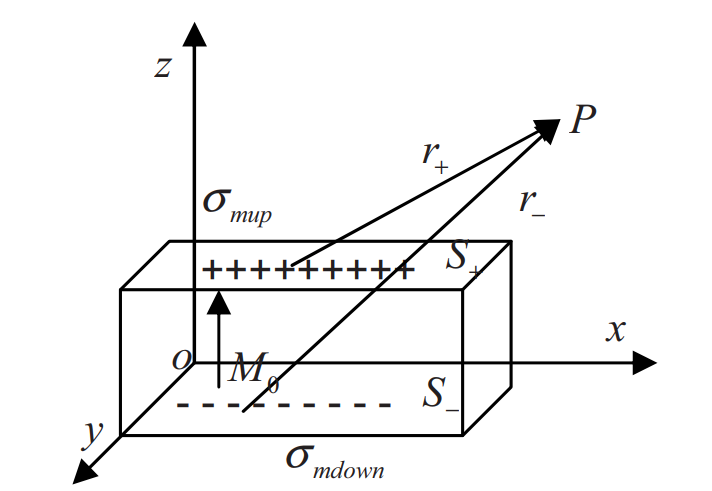
\includegraphics[width=0.5\textwidth]{Magnetic surface charge_2}
\caption{مدل بار مغناطیسی سطحی \cite{RN44}}
\label{fig:Magnetic surface charge}
\end{figure}

\subsection{مدل بار مغناطیسی نقطه‌ای}
در روش بار نقطه‌ای برای تحلیل میدان مغناطیسی، فرض می‌شود که توزیع بار مغناطیسی در یک حجم به‌صورت متمرکز در هشت نقطه در گوشه‌های آن حجم قرار گرفته است. با این فرض، اثر مغناطیسی این جسم می‌تواند به‌صورت مجموع آثار هر یک از بارهای نقطه‌ای محاسبه شود. این رویکرد امکان محاسبه‌ی دقیق شدت میدان مغناطیسی و نیروی وارد بر یک جسم خارجی را فراهم می‌آورد. از طریق محاسبه‌ی میدان‌های ناشی از هر بار نقطه‌ای و جمع آنها، میدان مغناطیسی کل حاصل می‌شود و به این ترتیب، شدت میدان مغناطیسی ناشی از آهنربای دائمی به کمک این روش به‌طور دقیق محاسبه می‌گردد. در ادامه، معادلات مربوط به محاسبه‌ی شدت میدان مغناطیسی ناشی از هر بار نقطه‌ای ارائه شده‌است.
\begin{align}
B_{xk} &= \frac{\epsilon_k}{4\pi} \ln\left(-y_r + \sqrt{x_r^2 + y_r^2 + z_r^2}\right), \\
B_{yk} &= \frac{\epsilon_k}{4\pi} \ln\left(-x_r + \sqrt{x_r^2 + y_r^2 + z_r^2}\right), \\
B_{zk} &= \frac{\epsilon_k}{4\pi} \arctan\left( \frac{x_r y_r}{\sqrt{x_r^2 + y_r^2 + z_r^2}} \right),
\end{align}

\begin{figure}[ht]
\centering
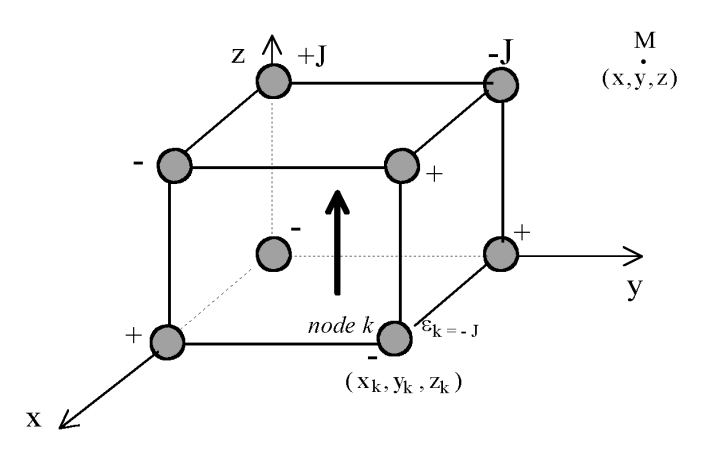
\includegraphics[width=0.5\textwidth]{Magnetic_Node}
\caption{مدل بار مغناطیسی نقطه‌ای \cite{RN44}}
\label{figMagnetic_Node}
\end{figure}

\subsection{مدل های مبتنی بر داده}

در این روش‌ها، به‌جای مدل‌سازی دقیق ساختار فیزیکی دستگاه و استخراج معادلات دینامیکی آن، پارامترهای مورد نیاز مانند شدت میدان مغناطیسی از طریق داده‌های تجربی یا شبیه‌سازی المان محدود (FEM) تخمین زده می‌شوند. این رویکرد مبتنی بر داده نیازمند دسترسی به اطلاعات دقیق از سیستم واقعی یا شبیه‌سازی کامل آن است تا بتوان دقت و اعتبار تخمین‌ها را ارزیابی کرد. در پژوهش 
\cite{RN10}
، برای تخمین شدت میدان مغناطیسی آرایه هالباخ دوبعدی از معادلات هارمونیک و سری فوریه استفاده شده است. تغییرات میدان مغناطیسی تولیدشده توسط این آرایه به‌صورت موجی سینوسی مدل‌سازی شده است، اما این روش تنها زمانی دقیق است که فرض شود سطح آرایه به‌صورت نامحدود ادامه دارد. برای حل این مشکل، آرایه به سه ناحیه مرکزی، کناری و گوشه‌ای تقسیم‌بندی شده و برای هر ناحیه هارمونیک‌های مجزا در نظر گرفته شده است. نتایج این پژوهش نشان می‌دهند که با استفاده از سه هارمونیک اول، می‌توان میدان مغناطیسی را در نواحی کناری و گوشه‌ای با دقت مناسبی تخمین زد.

\begin{figure}[ht]
\centering 
\subfloat[\cite{RN10}]{
\label{fig:harmonic_1}
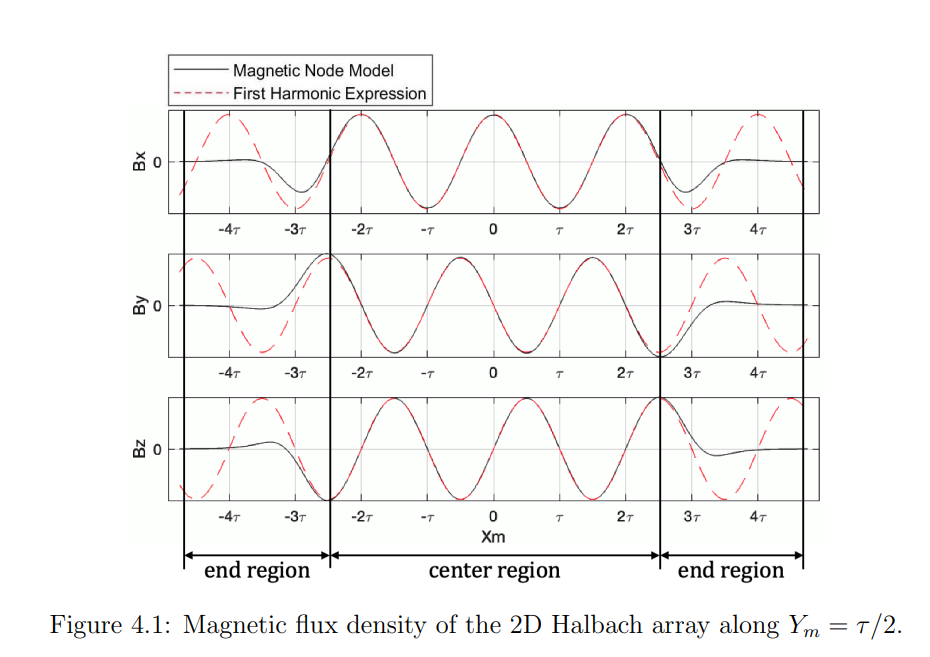
\includegraphics[width=0.45\textwidth]{harmonic_1}}
\hspace{2mm}
\subfloat[\cite{RN10}]{
\label{fig:harmonic_2}
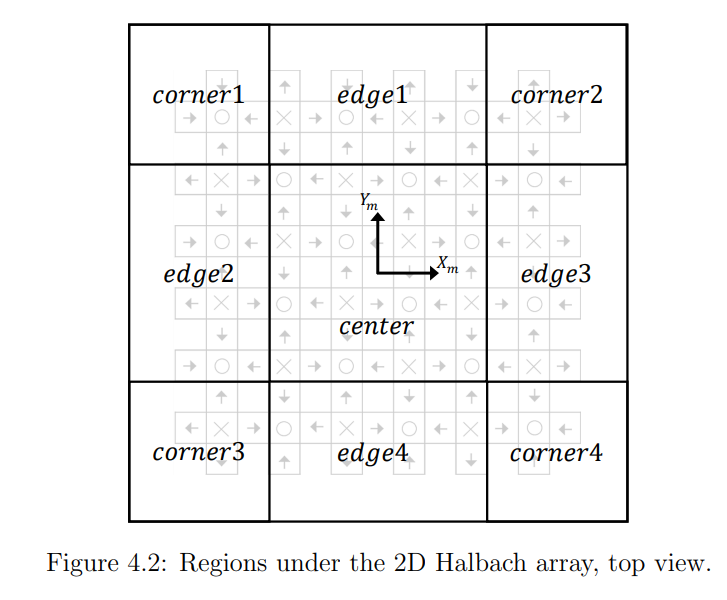
\includegraphics[width=0.45\textwidth]{harmonic_2}}
\caption{مدل هارمونیک}
\label{fig:harmonic}
\end{figure}



!
را در فایل 
\lr{main.tex}،
غیرفعال%
\footnote{
برای غیرفعال کردن یک دستور، کافی است در ابتدای آن، علامت درصد انگلیسی (\%) بگذارید.
}
 کنید. در غیر این صورت، ابتدا مطالب دو فصل اول پردازش شده و سپس مطالب فصل ۳ پردازش می‌شود که این کار باعث طولانی شدن زمان پردازش می‌گردد. هر زمان که خروجی کل \پ را خواستید، تمام فصل‌ها را دوباره در
\lr{main.tex}
فعال نمائید.
بدیهتاً لازم نیست فصل‌های \پ را به ترتیب تایپ کنید. مثلاً می‌توانید ابتدا مطالب فصل ۳ را تایپ نموده و سپس مطالب فصل ۱ را تایپ کنید. 
\subsubsection{مراجع}
برای وارد کردن مراجع \پ کافی است فایل 
\lr{MyReferences.bib}
را باز کرده و مراجع خود را به شکل اقلام نمونهٔ داخل آن، وارد کنید.  سپس از \lr{bibtex} برای تولید مراجع با قالب مناسب استفاده نمائید. برای توضیحات بیشتر بخش \ref{Sec:Ref} از پیوست \ref{app:latexIntro} و نیز پیوست \ref{app:refMan} را ببینید.

\subsubsection{واژه‌نامه فارسی به انگلیسی و برعکس}
برای وارد کردن معادل فارسی اصطلاحات لاتین در متن و تهیه فهرست واژه‌نامه از آنها، از بستهٔ
\lr{glossaries}
و نرم‌افزار
\lr{xindy}
استفاده می‌شود. بدین منظور کافی است اصطلاحات لاتین و ترجمهٔ آنها را در فایل
\lr{words.tex}
وارد کرده و هر جای متن که خواستید با دستورات
\verb|gls{label}|
یا \verb|glspl{label}|
معادل فارسی مفرد یا جمع یک اصطلاح را بیاورید.

مثلا در اینجا، واژهٔ
«\gls{Action}»
برای بار اول و دوباره
«\gls{Action}»
برای بار دوم در متن ظاهر شده است.
جهت توضیحات بیشتر به پیوست
\ref{app:refMan}
مراجعه کنید.
\subsubsection{نمایه}
برای وارد کردن نمایه، باید از 
\lr{xindy}
استفاده کنید. 
%زیرا 
%\lr{MakeIndex}
%با حروف «گ»، «چ»، «پ»، «ژ» و «ک» مشکل دارد و ترتیب الفبایی این حروف را رعایت نمی‌کند. همچنین، فاصله بین هر گروه از کلمات در 
%\lr{MakeIndex}،
%به درستی رعایت نمی‌شود که باعث زشت شدن حروف‌چینی این قسمت می‌شود. 
راهنمای چگونگی کار با 
\lr{xindy} 
را می‌توانید در ویکی پارسی‌لاتک و یا مثالهای موجود در دی‌وی‌دی «مجموعه پارسی‌لاتک»، پیدا کنید.

\subsection{اگر سوالی داشتم، از کی بپرسم؟}
برای پرسیدن سوال‌های خود موقع حروف‌چینی با زی‌پرشین، می‌توانید به
\href{http://qa.parsilatex.com}{سایت پرسش و پاسخ پارسی‌لاتک}%
\LTRfootnote{http://qa.parsilatex.com}
یا
\href{http://forum.parsilatex.com}{بایگانی تالارگفتگوی قدیمی پارسی‌لاتک}%
\LTRfootnote{http://forum.parsilatex.com}
مراجعه کنید. شما هم می‌توانید روزی به سوال‌های دیگران در اینترنت جواب دهید.
بستهٔ زی‌پرشین و بسیاری از بسته‌های مرتبط با آن مانند
\lr{bidi} و
\lr{Persian-bib}،
مجموعه پارسی‌لاتک، مثالهای مختلف موجود در آن، قالب پایان‌نامه دانشگاههای مختلف و سایت پارسی‌لاتک همه به صورت داوطلبانه توسط افراد گروه پارسی‌لاتک و گروه
\lr{Persian TeX}
و بدون هیچ کمک مالی انجام شده‌اند. کار اصلی نوشتن و توسعه زی‌پرشین توسط آقای وفا خلیقی انجام شده است که این کار بزرگ را به انجام رساندند.
اگر مایل به کمک به گروه پارسی‌لاتک هستید به سایت این گروه مراجعه فرمایید:
\begin{center}
	\url{http://www.parsilatex.com}
\end{center}

\section{محتویات فصل اول یک پایان‌نامه}
فصل اول یک پایان‌نامه باید به مقدمه یا کلیات تحقیق بپردازد.
هدف از فصل مقدمه%
\LTRfootnote{Introduction}،
شرح مختصر مسأله تحقیق، اهمیت و انگیزه محقق از پرداختن به آن موضوع، بهمراه اشاره‌ای کوتاه به روش و مراحل تحقیق است. مقدمه، اولین فصل از ساختار اصلی \پ بوده و زمینه اطلاعاتی لازم را برای خواننده فراهم می‌آورد. در طول مقدمه باید سعی شود موضوع تحقیق با زبانی روشن، ساده و بطور عمیق و هدفمند به خواننده معرفی شود. این فصل باید خواننده را مجذوب و اهمیت موضوع تحقیق را آشکار سازد. در مقدمه باید با ارائهٔ سوابق، شواهد تحقیقی و اطلاعات موجود (با ذکر منبع) با روشی منظم، منطقی و هدف‌دار، خواننده را جهت داد و به سوی راه حل مورد نظر هدایت کرد. مقدمه مناسب‌ترین جا برای ارائهٔ اختصارات و بعضی توضیحات کلی است، توضیحاتی که شاید نتوان در مباحث دیگر آنها را شرح داد.

مقدمه، یکی از ارکان اساسی و اصلی پایان نامه است که مهمترین قسمت‌های آن عبارتند از: 

\subsection{عنوان تحقیق} 
باید شناختی دقیق و روشن از حوزهٔ موضوع تحقیق را عرضه دارد و خالی از هرگونه ابهام و پیچیدگی باشد.

\subsection{مسأله تحقیق}
وظیفه اصلی مقدمه بیان این مطلب به خواننده است که چرا انجام تحقیق را به عهده گرفته‌اید. اگر دلیل شما برای انجام این کار پاسخگویی به سؤال مورد علاقه‌تان است، با مشکل زیادی روبه‌رو نخواهید بود. یکی از بهترین روش‌ها برای نوشتن مقدمهٔ یک پایان‌نامه، طرح پرسش یا پرسش‌هایی مهم و اساسی است که کار تحقیقاتی شما از آغاز تا پایان قصد پاسخ دادن به آن را دارد. گاهی می‌توانید ابتدا اهمیت موضوع را بیان و سپس پرسش خود را در آن موضوع مطرح کنید.

\subsection{تاریخچه‌ای از موضوع تحقیق}
به طور کلی تشریح روندهای تحقیقاتی در محدودهٔ مورد مطالعه، مستلزم ارجاع به کارهای دیگران است. بعضی از نویسندگان برای کارهای دیگران هیچ اعتباری قائل نمی‌شوند و در مقابل، بعضی دیگر از نویسندگان در توصیف کارهای دیگران، بسیار زیاده‌روی می‌کنند. اکثر مواقع، ارجاع به مقالات دو سال قبل از کارتان، بهتر از نوشتن سطرهای مرجع است. در این قسمت باید به طور مختصر به نظرات و تحقیقات مربوط به موضوع و یا مسائل و مشکلات حل نشده در این حوزه و همچنین توجه و علاقه جامعه به این موضوع، اشاره شود.

\subsection{تعریف موضوع تحقیق}
در این قسمت محقق، موضوع مورد علاقه و یا نیاز احساس شدهٔ خود را در حوزه تحقیق بیان می‌دارد و عوامل موجود در موقعیت را تعریف و تعیین می‌کند.

\subsection{هدف یا هدف‌های کلی و آرمانی تحقیق}
این قسمت باید با جملات مثبت و کلی طرح شود و از طولانی شدن مطالب پرهیز شود.

\subsection{روش انجام تحقیق}
در این قسمت، پژوهشگر روش کاری خود را بیان می‌دارد و شیوه‌های گوناگونی را که در گردآوری مطالب خود بکار برده، ذکر می‌کند. همچنین اگر روش آماری خاصی را در تهیه و تدوین اطلاعات به کار برده است، آن شیوه را نیز اینجا بیان می‌کند.

\subsection{نوآوری، اهمیت و ارزش تحقیق}
در این قسمت، در مورد نوآوری علمی و عملی تحقیق که محقق به آن دست خواهد یافت، بحث می‌شود. ممکن است لازم باشد تا برخی نمودارهای خلاصه در این بخش استفاده شوند. به عنوان مثال، نموداری از مقاله
\cite{kim2016integrated}
در شکل
\ref{fig:sampleDiagram}
آمده است.
\begin{figure}[ht]
	\centerline{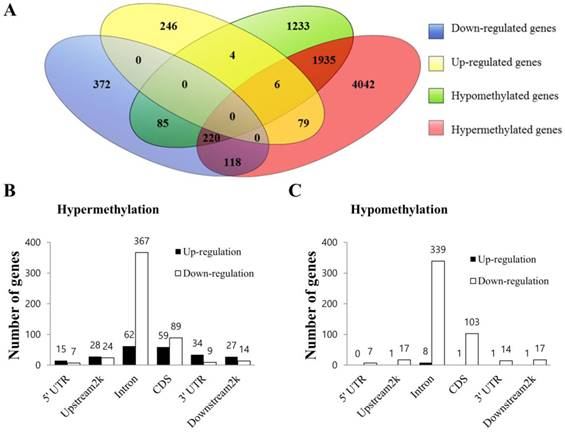
\includegraphics[width=0.8\textwidth]{journal-of-cancer_sample-result}}
	\caption{یک نمونه نمودار خلاصه برای نمایش نوآوری در نتایج
		%\cite{kim2016integrated}
	}
	\label{fig:sampleDiagram}
\end{figure}\\
طبیعتاً به صلاحدید نگارنده، شکل‌ها و نمودار‌ها می توانند در بخش های مختلف، خصوصا فصل
\ref{chap:results}
مورد استفاده قرار گیرند.

\subsection{تعریف واژه‌ها (اختیاری)}
در این قسمت محقق باید واژه‌هایی را که ممکن است برای خواننده آشنا نباشد، تعریف کند.

\subsection{خلاصه فصل‌ها}
در آخرین قسمتِ فصل اول پایان‌نامه، خلاصه‌ای اشاره‌وار از فصل‌های آتی آورده می‌شود تا خواننده بتواند تصویری واضح از دیگر قسمت‌های پایان‌نامه در ذهن خود ترسیم کند.

\section{جمع‌بندی}
در این فصل به دو مقولهٔ نحوه استفاده از قالب \پ دانشگاه تهران و نیز ویژگی‌هایی که محتویات فصل اول پایان‌نامه (یعنی مقدمه) باید داشته باشند، پرداخته شد. با توجه به اینکه این راهنما نحوه استفاده از قالب را شرح داده، ملزومات محتوایی هر فصل پایان‌نامه را توضیح می‌دهد و در پیوست‌ها نیز نحوهٔ کار با لاتک را یادآوری خواهد کرد، بنابراین مطالعهٔ کامل آن مقداری وقت شما را خواهد گرفت؛ اما مطمئن باشید از اتلاف وقت شما در ادامه کارتان تا حد زیادی جلوگیری خواهد کرد. در نوشتن متن حاضر سعی شده است علاوه بر ایجاد یک قالب لاتک برای پایان‌نامه‌های دانشگاه تهران، نکات محتوایی هر فصل نیز گوشزد گردد. طبیعتاً برای نگارش پایان‌نامهٔ خود می‌بایست مطالب تمام فصل‌ها را خودتان بازنویسی کنید.

در ادامهٔ این راهنما، تنها فصل‌هایی که یک پایان‌نامه باید داشته باشد و نیز خصوصیات یا ساختاری که محتویات هر فصل باید از آنها برخوردار باشد%
\footnote{از روی فایل «تمپلیت نگارش و تدوین پایان‌نامه \cite{UTThesisGuide}»}،
آورده می‌شوند. نهایتاً  در پیوست‌ها، مطالبی در باب یادآوری دستورات لاتک، نحوه نوشتن فرمول‌ها، تعاریف، قضایا، مثال‌ها، درج تصاویر، نمودارها، جداول و الگوریتم‌ها و نیز مدیریت مراجع، آمده است.

همچنین توصیه اکید دارم که رفع خطاهایی که احتمالاً با آنها مواجه می‌شوید را به آخر موکول نفرمایید و به محض برخورد با خطا، آن را اشکال‌زدایی و برطرف نمائید.		% فصل اول: مقدمه
%% !TeX root=../main.tex
\setcounter{topnumber}{5}      % Increase number of floats at the top of the page
\setcounter{totalnumber}{5}    % Increase total number of floats on a page
\renewcommand{\floatpagefraction}{.8}  % Allow more of the page to be taken up by floats

\chapter{مروری بر مطالعات انجام شده}
%\thispagestyle{empty} 
\section{مقدمه}
در این فصل، پژوهش‌های پیشین در زمینه‌ی موتورهای مسطح مبتنی بر شناوری مغناطیسی (MLPM) با تمرکز بر ویژگی‌های اساسی آنان که به طور کلی در بخش‌های زیر دسته‌بندی شده‌اند، مورد بررسی قرار می‌گیرند. 
\begin{itemize}
	\item
		\textit{معماری دستگاه}:
بررسی انواع معماری‌های موجود برای MLPM و تأثیر آن‌ها بر عملکرد کلی سیستم.
	\item
		\textit{ساختار آهنرباهای دائمی و الکتریکی}:
مرور انواع آهنرباهای الکتریکی و چینش‌های مختلف آهنربا‌های دائمی و نقش آن‌ها در بهینه‌سازی عملکرد سیستم.
	\item
		\textit{طراحی کنترلر}:
معرفی روش‌های کنترل کلاسیک و مدرن برای این سیستم‌ها و چگونگی بهبود پایداری و دقت حرکت.
	\item
		\textit{روش‌های شناسایی سیستم و مدل‌سازی دینامیکی}:
تحلیل روش‌های شناسایی و تخمین مدل‌های دینامیکی سیستم برای شبیه‌سازی و بهینه‌سازی عملکرد.
\end{itemize}
در بخش‌های بعد، پژوهش‌های انجام‌شده بر اساس این ویژگی‌ها ارزیابی شده و مزایا و معایب هر روش مورد بررسی قرار می‌گیرد.

\section{معماری دستگاه‌های MLPM}
سیستم‌های شناوری مغناطیسی به دلیل ماهیت ناپایدارشان بدون استفاده از حلقه‌های کنترلی نمی‌توانند پایداری لازم را فراهم کنند. به همین دلیل، در تمامی ساختارهای پیشنهادی، از سیم‌پیچ‌های الکتریکی برای تولید میدان مغناطیسی با شدت کنترل ‌شده استفاده می‌شود. این سیم‌پیچ‌ها وظیفه دارند تا موقعیت جسم معلق را پایدار کرده و آن را در حالت مطلوب نگه ‌دارند.

در طراحی موتورهای مسطح، که از دو بخش ثابت
\LTRfootnote{Stator}
 و متحرک
\LTRfootnote{Mover}
تشکیل شده‌اند، امکان تغییر در طراحی و محل قرارگیری آهنرباهای الکتریکی و دائمی وجود دارد. نیروی مغناطیسی وارد بر بخش متحرک می‌تواند به‌صورت جاذبه‌ای از بالا یا دافعه‌ای از پایین اعمال شود. با این حال، در موتورهای مسطح به دلیل لزوم کم بودن فاصله میان سیم‌پیچ‌ها و اجسام معلق، اعمال نیروی جاذبه‌ای از بالا امکان‌پذیر نیست. به همین دلیل، در تمامی طراحی‌ها، نیروی مغناطیسی دافعه‌ای از سمت پایین به بخش متحرک وارد می‌شود که امکان جابه‌جایی اجسامی که بر روی آنها قرار می‌گیرند را فراهم می‌کند.

با توجه به این موارد، دو طراحی کلی برای ساخت دستگاه‌های MLPM ارائه می‌شود که در ادامه بررسی می‌‌شوند.
\subsection{سیم‌پیچ‌های متحرک و آهنرباهای ثابت}

در این معماری، بخش استاتور از مجموعه‌ای آهنربای ثابت تشکیل شده که میدان مغناطیسی پایدار در محیط اطراف خود ایجاد می‌کنند. بخش متحرک دستگاه شامل سیم‌پیچ‌هایی است که با عبور جریان الکتریکی از آن‌ها، میدان مغناطیسی متغیری تولید می‌گردد. این جریان به گونه‌ای تنظیم می‌شود که نیروی وارد بر آهنرباهای دائمی به‌دقت کنترل شود. طبق قانون سوم نیوتن، نیروهای وارد بر سیم‌پیچ‌ها و آهنرباهای دائمی به‌عنوان عمل و عکس‌العمل رفتار می‌کنند؛ به این ترتیب، نیرویی که به آهنرباها اعمال می‌شود، باعث ایجاد نیرویی برابر و در جهت مخالف بر سیم‌پیچ‌ها خواهد شد.

در پژوهش 
\cite{RN49}
، از ساختاری با سیم‌پیچ‌های چندلایه متعامد در بخش متحرک استفاده شده است. لایه اول سیم‌پیچ‌ها نیرویی را در راستاهای x و z ایجاد می‌کند، در حالی که لایه دوم نیرو را در راستاهای y و z اعمال می‌کند. این جداسازی نیروها به بهبود کنترل سیستم کمک می‌کند. علاوه بر این، به دلیل تفاوت فاصله میان لایه‌ها و استاتور، نیروهای تولیدشده توسط هر لایه متفاوت خواهند بود. راهکار ارائه‌شده برای این چالش، افزایش ضخامت لایه‌های دورتر از استاتور است. با این حال، برای جلوگیری از مشکلات ناشی از تفاوت ضخامت لایه‌ها، ساختاری سه‌لایه طراحی شده که ضمن افزایش نیروی تولیدی، ضخامت یکنواختی را در تمامی راستاها فراهم می‌نماید. در شکل 
\ref{fig:Multilayer_Mover_Coil}
ساختار این دستگاه نمایش داده شده است.

در پژوهش 
\cite{RN38}
، بخش متحرک از یک لایه سیم‌پیچ با چینش متعامد تشکیل شده که قابلیت اعمال نیرو در سه راستا را فراهم می‌سازد. در ادامه، پژوهش
\cite{RN14}
 روشی تحلیلی برای بهینه‌سازی ضخامت این سیم‌پیچ‌ها ارائه کرده است که با در نظر گرفتن معیارهای مختلف، به بهبود عملکرد سیستم می‌پردازد. شکل 
\ref{fig:Single_layer_Mover_Coil}
 این ساختار را نمایش داده است.

\begin{figure}[ht]
\centering 
\subfloat[استفاده از سیم‌پیچ‌های چندلایه
\cite{RN49}]
{ \label{fig:Multilayer_Mover_Coil}
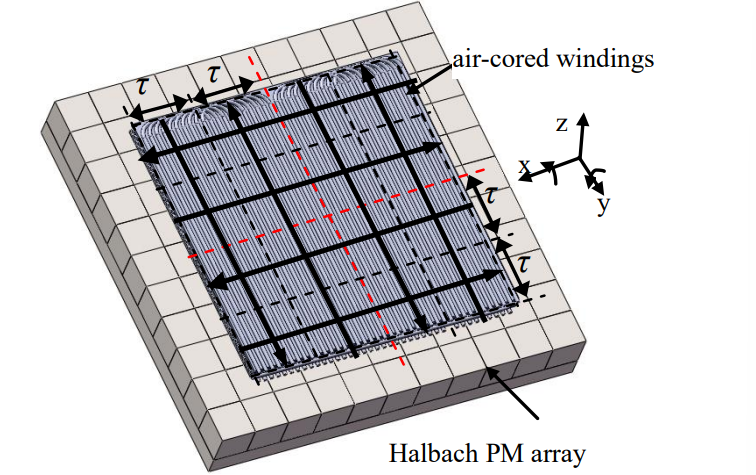
\includegraphics[width=0.5\textwidth]{Multilayer_Mover_Coil}}
%\hspace{2mm}
\subfloat[استفاده از سیم‌پیچ‌های یک لایه متعامد
\cite{RN14}]
{ \label{fig:Single_layer_Mover_Coil}
\includegraphics[width=0.5\textwidth]{Single_layer_Mover_Coil}}%
\caption{ساختار سیستم‌های MLPM با سیم‌پیچ‌های متحرک و آهنربای ثابت}
\label{fig:Moveing_Coil} %% label for entire figure
\end{figure}

با وجود اینکه این معماری امکان دستیابی به شناوری پایدار و حرکت با شش درجه آزادی را فراهم می‌کند، اما در کاربردهای عملی با محدودیت‌هایی مواجه است که بر عملکرد نهایی سیستم تأثیرگذار هستند. نخستین محدودیت، نیاز به تأمین انرژی الکتریکی برای سیم‌پیچ‌ها از طریق سیم‌های فیزیکی است که این امر به‌طور اجتناب‌ناپذیری ارتباط فیزیکی میان جسم متحرک و محیط اطراف را برقرار می‌سازد، در نتیجه حرکت آزادانه کامل جسم متحرک محدود می‌شود. دومین محدودیت، چالش خنک‌کاری سیم‌پیچ‌ها است که به دلیل ماهیت متحرک و معلق بودن آن‌ها، اجرای یک سیستم خنک‌کننده کارآمد دشوار خواهد بود. این مشکلات، نیاز به ارائه معماری جدیدی را آشکار می‌کند که بتواند این چالش‌ها را برطرف سازد.

\subsection{‌آهنرباهای متحرک و سیم‌پیچ‌های ثابت}

معماری دیگری که برای طراحی دستگاه‌های MLPM ارائه شده است، شامل قرار دادن سیم‌پیچ‌ها در بخش استاتور و استفاده از آهنرباهای دائمی در بخش متحرک می‌باشد. این ساختار نوین که در بسیاری از پژوهش‌ها مورد استفاده قرار گرفته، مشکلات معماری‌های پیشین مانند محدودیت جابه‌جایی متحرک ناشی از اتصالات فیزیکی و چالش‌های خنک‌کاری سیم‌پیچ‌ها را برطرف کرده و منجر به بهبود عملکرد کلی سیستم شده است.

در پژوهش 
\cite{RN7}
 استاتوری با چینش سیم‌پیچ‌ها مطابق با الگوی شاه‌ماهی
\LTRfootnote{Herringbone pattern}
 طراحی و پیاده‌سازی شده است. این طراحی امکان اعمال نیروی مغناطیسی به دو آهنربای دیسکی تعبیه‌شده در بخش متحرک را فراهم کرده است که دقتی در حدود 1 درجه در زوایای حرکت و 1 میلی‌متر در موقعیت متحرک به دست آورده است
\cite{RN7}
. در ادامه این پژوهش، ساختاری جدید برای بخش متحرک ارائه شده که شامل 6 آهنربای دیسکی با چینش کروی و فواصل ثابت می‌باشد. این طراحی توانسته است چرخش آزادانه متحرک را حول سه محور ممکن سازد 
\cite{RN39}.
شکل (
\ref{fig:Moving_Magnet_1})
همچنین در پژوهش 
\cite{RN62}
 نیز از این چینش سیم‌پیچ‌ها استفاده شده و مطابق با شبیه‌سازی‌های ارائه شده، مزیت آنان در ایجاد میدان مغناطیسی یکنواخت‌تر در نواحی کناری سیم‌پیچ‌ها نمایش داده شده است.

استفاده از سیم‌پیچ‌های سه‌فاز به‌جای تغذیه با جریان مستقیم، رویکردی است که در پژوهش 
\cite{RN24}
معرفی و اجرا شده است. در این ساختار، چهار آرایه از سیم‌پیچ‌های سه‌فاز، همان‌طور که در 
شکل (
\ref{fig:Moving_Magnet_2})
 نشان داده شده است، به‌گونه‌ای طراحی شده‌اند که نیروی مغناطیسی لازم را تولید کنند.

به ‌منظور کاهش هزینه‌ی محاسباتی در جابه‌جایی‌های طولانی، پژوهش 
\cite{RN32}
 ساختاری را ارائه کرده است که از دو مجموعه سیم‌پیچ‌ سه‌فاز و تک‌فاز تشکیل شده است. در این طراحی، کنترل حرکت در مسافت‌های طولانی توسط سیم‌پیچ‌های سه‌فاز انجام می‌پذیرد، در حالی که برای تنظیم دقیق موقعیت متحرک در صفحه، از سیم‌پیچ‌های تک‌فاز بهره برده می‌شود.
شکل (
\ref{fig:Moving_Magnet_3})

استفاده از سیم‌پیچ‌های ماژولار در طراحی استاتورهایی با چینش دوبعدی، رویکردی است که در دستگاه‌های MagTable و MagFloor از دانشگاه واترلو پیاده‌سازی شده است
\cite{RN8,RN30,RN10}
 در این طراحی، ماژول‌هایی از سیم‌پیچ‌های با سطح مقطع مربع به‌گونه‌ای طراحی شده‌اند که با قرار گرفتن در کنار یکدیگر، فضای کاری نامحدودی برای جابه‌جایی متحرک فراهم می‌کنند.(شکل
\ref{fig:Moving_Magnet_4})
 همچنین، پژوهش
\cite{RN8}
 نشان داده است که آهنرباهای با سطح مقطع مربع، در مقایسه با سیم‌پیچ‌های دایروی با جریان الکتریکی مشابه، می‌توانند شدت میدان مغناطیسی بیشتری ایجاد کنند، که این مزیت عملکرد کلی سیستم را بهبود می‌بخشد.

\begin{figure}[ht]
\centering 
\subfloat[الگوی شاه‌ماهی سیم‌پیچ‌ها
\cite{RN39}]
{ \label{fig:Moving_Magnet_1}
\includegraphics[width=0.45\textwidth]{Moving_Magnet_1}}
\hspace{2mm}
\subfloat[سیم‌پیچ‌های سه فاز
\cite{RN24}]
{ \label{fig:Moving_Magnet_2}
\includegraphics[width=0.45\textwidth]{Moving_Magnet_2}}
\\ % Newline to wrap the figures to the next row
\subfloat[ساختار دوگانه سیم‌پیچ‌ها
\cite{RN32}]
{ \label{fig:Moving_Magnet_3}
\includegraphics[width=0.45\textwidth]{Moving_Magnet_3}}
\hspace{2mm}
\subfloat[ساختار ماژولار سیم‌پیچ‌ها
\cite{RN10}]
{ \label{fig:Moving_Magnet_4}
\includegraphics[width=0.45\textwidth]{Moving_Magnet_4}}
\label{fig:Moveing_Magnet} %% label for entire figure
\caption{ساختارهای آهنرباهای متحرک و سیم‌پیچ‌های ثابت}
\end{figure}








\section{ساختار آهنرباهای دائمی}

همان‌طور که در بخش قبل اشاره شد، میدان مغناطیسی کنترل‌شده توسط آهنرباهای الکتریکی ایجاد می‌شود و بر اثر تعامل این میدان متغیر با میدان ثابت آهنرباهای دائمی، نیرویی بر بخش متحرک دستگاه وارد می‌شود که حرکت آن را در راستاهای مختلف ممکن می‌سازد. بنابراین، طراحی بهینه آهنرباهای دائمی، به‌ویژه برای تولید میدان مغناطیسی قوی‌تر با کمترین وزن، در بهبود کارایی دستگاه نقش کلیدی دارد. در این بخش، طراحی‌های مختلف آهنرباهای دائمی که در پژوهش‌های پیشین ارائه شده‌اند، با تمرکز بر بهینه‌سازی این ویژگی‌ها بررسی می‌شوند.
\subsection{استفاده از آهنرباهای دیسکی}

استفاده از آهنرباهای دیسکی رویکردی ساده و مؤثر برای ایجاد میدان مغناطیسی دائمی محسوب می‌شود. با انتخاب موادی با خاصیت مغناطیسی بالا، مانند آهنرباهای نئودیمیومی، می‌توان به شدت میدان مغناطیسی مطلوب دست یافت. به عنوان نمونه، در پژوهش 
\cite{RN7}
 از دو آهنربای دیسکی جهت تأمین میدان مغناطیسی ثابت استفاده شده است. همچنین در پژوهش 
\cite{RN39}
 با به‌کارگیری ۶ آهنربای دیسکی، امکان چرخش آزادانه حول سه محور فراهم شده است.(شکل
\ref{fig:Disk_Magnet_1})
 در پژوهش 
\cite{RN8}
 نیز از ترکیب‌های متفاوتی از آهنرباهای دیسکی برای بخش متحرک دستگاه استفاده شده است، که این ترکیب‌ها شامل تغییر اندازه‌ی یک آهنربا و استفاده از سه آهنربای دیسکی است. سیستم شناوری مغناطیسی با پنج درجه آزادی که تنها از یک آهنربای دیسکی تشکیل شده است، در پژوهش 
\cite{RN62}
 به عنوان نمونه‌ای موفق از این رویکرد معرفی شده است. این طراحی، با وجود سادگی معماری، توانسته نتایج رضایت‌بخشی را از نظر عملکرد ارائه دهد و نشان می‌دهد که استفاده از آهنربای دیسکی، علاوه بر سادگی، می‌تواند در کاربردهای مختلف به‌ویژه در سیستم‌های با نیاز به دقت بالا و چند درجه آزادی، کارآمد باشد. شکل((
\ref{fig:Disk_Magnet_2})


\begin{figure}[ht]
\centering 
\subfloat[دو آهنربای دیسکی
\cite{RN7}]
{ \label{fig:Disk_Magnet_1}
\includegraphics[width=0.5\textwidth]{Disk_Magnet_1}}
%\hspace{2mm}
\subfloat[یک آهنربای دیسکی
\cite{RN62}]
{ \label{fig:Disk_Magnet_2}
\includegraphics[width=0.5\textwidth]{Disk_Magnet_2}}%
\caption{استفاده از آهنربای دیسکی در طراحی متحرک}
\label{fig:Disk_Magnet} %% label for entire figure
\end{figure}



\subsection{آرایه‌ی هالباخ یک بعدی}

آرایه‌ی هالباخ
\LTRfootnote{Halbach Array}
 به‌عنوان چینشی از آهنرباهای دائمی تعریف می‌شود که در آن جهت مغناطیس‌شوندگی هر آهنربا با آهنربای مجاور خود ۹۰ درجه تفاوت دارد. این آرایه به‌طور خاص قادر است میدان مغناطیسی در یک سوی آرایه را خنثی کرده و در سوی دیگر میدان را به میزان تقریبی 1.4 برابر افزایش دهد.
مزیت این ساختار در طراحی سیستم‌های MLPM، توانایی آن در تولید شدت میدان مغناطیسی بیشتر است. به‌همین‌دلیل، این چینش در بسیاری از پژوهش‌ها مورد استفاده قرار گرفته است.
با این حال، استفاده از تنها یک آرایه‌ی یک‌بعدی هالباخ به‌تنهایی نمی‌تواند نیرویی در دو راستای افقی ایجاد کند. لذا معمولاً از تعداد بیشتری از این آرایه‌ها در ساختار متحرک استفاده می‌شود. به‌عنوان مثال، در پژوهش‌های 
\cite{RN24,RN27}
 از چهار آرایه‌ی هالباخ یک‌بعدی در بخش متحرک استفاده شده است که هر یک از این آرایه‌ها قادر به ایجاد نیرویی در یکی از راستاهای افقی و عمودی هستند.
در پژوهش 
\cite{RN39}
، مشابه آنچه که در بخش استاتور پیاده‌سازی شده بود، از ساختار دوگانه‌ای در بخش متحرک بهره‌برداری شده است، به‌گونه‌ای که دو مجموعه چهارگانه از آرایه‌های هالباخ در معماری این بخش به‌کار رفته‌اند.

\begin{figure}[ht]
\centering 
\subfloat[آرایه‌ی هالباخ
\cite{RN16}]
{ \label{fig:halbach1D}
\includegraphics[width=0.5\textwidth]{halbach1D}}
%\hspace{2mm}
\subfloat[4 آرایه‌ی یک بعدی هالباخ
\cite{RN39}]
{ \label{fig:4_halbach1D_array}
\includegraphics[width=0.5\textwidth]{4_halbach1D_array}}%
\caption{آرایه هالباخ یک‌بعدی}
\label{fig:halbach1D} %% label for entire figure
\end{figure}

\subsection{آرایه هالباخ دوبعدی}

برای رفع محدودیت‌های آرایه‌ی هالباخ یک‌بعدی که تنها در یک راستا نیرو ایجاد می‌کند، ساختار جدیدی از آرایه‌ی دوبعدی ارائه شده است. این آرایه قادر است میدان مغناطیسی را در یک طرف صفحه حذف و در طرف دیگر تقویت کند. با این ویژگی، استفاده از چندین آرایه برای تأمین میدان مغناطیسی ثابت ضروری نخواهد بود. طراحی آرایه‌ی دوبعدی در بسیاری از پژوهش‌ها برای بخش‌های متحرک یا استاتور سیستم‌های MLPM به کار گرفته شده است.

استفاده از آرایه‌ی هالباخ در پژوهش‌های مختلفی از جمله
\cite{RN10, RN30} 
و
\cite{RN55, RN26} 
نشان‌دهنده‌ی عملکرد بهینه‌ی این معماری در بخش متحرک سیستم‌های MLPM است.(شکل
\ref{fig:halbach2D_2})
 همچنین در پژوهش
\cite{RN14}
 از این آرایه به عنوان بخشی از استاتور دستگاه بهره‌گیری شده است. در 
\cite{RN61}
 ماژول‌هایی برای ساخت این آرایه استفاده شده (شکل
\ref{fig:halbach2D_4})
 و در
\cite{RN49}
 برای تشکیل آرایه از قطعات آهنی در فضای خالی میان آن استفاده شده است؛ اما این رویکرد باعث ایجاد خطا در دقت میدان مغناطیسی شده است. (شکل
\ref{fig:halbach2D_3})
علاوه بر این، در پژوهش
\cite{RN28}
، طراحی جدیدی با آهنرباهایی با میزان مغناطیس‌شوندگی و ارتفاع متفاوت پیشنهاد شده است.
\begin{figure}[ht]
\centering 
\subfloat[آرایه هالباخ دو بعدی و میدان مغناطیسی آن
\cite{RN10}]
{ \label{fig:halbach2D_2}
\includegraphics[width=0.45\textwidth]{halbach2D_2}}
\hspace{2mm}
\subfloat[آرایه هالباخ دوبعدی با قطعات آهنی در فضاهای خالی
\cite{RN49}]
{ \label{fig:halbach2D_3}
\includegraphics[width=0.45\textwidth]{halbach2D_3}}
\\ % Newline to wrap the figures to the next row
\subfloat[آرایه هالباخ دوبعدی ماژولار
\cite{RN61}]
{ \label{fig:halbach2D_4}
\includegraphics[width=0.45\textwidth]{halbach2D_4}}
\caption{آرایه هالباخ دو‌بعدی}
\label{fig:halbach2D} %% label for entire figure

\end{figure}
\section{طراحی کنترلر}
همان‌طور که پیش‌تر اشاره شد، سیستم‌های شناوری مغناطیسی ذاتاً ناپایدار هستند و برای دستیابی به پایداری، به کنترلری با عملکرد دقیق و خطای کم نیاز است. در پژوهش‌های مختلف، از کنترلرهای گوناگونی برای این سیستم‌ها بهره گرفته شده است؛ از جمله کنترلرهای کلاسیک نظیر PID، کنترلرهای مدرن مانند کنترل مبتنی بر پیش‌بینی مدل (MPC) و همچنین مدل‌های مبتنی بر هوش مصنوعی نظیر شبکه‌های بازگشتی GRU. در این بخش، به بررسی این کنترلرها و مقایسه‌ عملکرد آنها خواهیم پرداخت.
\subsection{کنترلر PID}

کنترل تناسبی-انتگرالی-مشتقی (PID) به عنوان یکی از پرکاربردترین و موثرترین کنترلرهای کلاسیک در سیستم‌های دینامیکی، گزینه‌ای مناسب برای کنترل سیستم‌های MLPM محسوب می‌شود. این کنترلر به دلیل سادگی در پیاده‌سازی، تنظیم دقیق و توانایی تنظیم خروجی سیستم بر اساس خطاهای ورودی، به‌طور گسترده در سیستم‌های مختلف استفاده شده است. برای کنترل سیستم‌های MLPM، به ازای هر درجه آزادی یک کنترلر PID طراحی و پیاده‌سازی می‌شود تا بتواند جریان الکتریکی سیم‌پیچ‌ها را تنظیم کرده و میدان مغناطیسی لازم برای ایجاد و حفظ موقعیت متحرک را تأمین کند.

در پژوهش‌های متعددی از کنترلر PID برای سیستم‌های MLPM بهره گرفته شده است. به عنوان مثال، در 
\cite{RN39,RN24}
از کنترلرهای PID ساده برای کنترل جریان سیم‌پیچ‌ها استفاده شده که وظیفه تنظیم میدان مغناطیسی و در نتیجه، کنترل موقعیت جسم متحرک را بر عهده دارند. علاوه بر این، در پژوهش
\cite{RN32}
، از دو کنترلر PID در یک ساختار دوگانه استفاده شده است. کنترلر اول برای جابه‌جایی‌های بلند و در مسافت‌های طولانی به کار رفته و جریان سیم‌پیچ‌های اصلی را تنظیم می‌کند، در حالی که کنترلر دوم برای حرکات دقیق کوتاه‌برد طراحی شده و کنترل جریان سیم‌پیچ‌های ثانویه را بر عهده دارد. این روش باعث بهینه‌سازی کنترل دقیق و بهبود دقت در حرکات کوتاه‌برد و جابه‌جایی‌های سریع می‌شود.
همچنین در سیستم MagTable، برای کنترل دقیق موقعیت آهنرباهای دائمی، از شش کنترلر PID به‌صورت همزمان استفاده شده است تا نیروی متوازن برای پایدارسازی موقعیت متحرک در چندین جهت فراهم شود 
\cite{RN8}
. این نوع طراحی و استفاده از کنترلرهای PID نشان می‌دهد که علی‌رغم محدودیت‌های موجود در کنترلرهای کلاسیک، این روش همچنان در بسیاری از سیستم‌های مغناطیسی پیچیده مانند MLPM کارایی بالایی دارد.

\begin{figure}[ht]
\centering{\includegraphics[width=0.5\textwidth]{PID_1}}
\caption{کنترلر PID با 6 درجه آزادی
\cite{RN8}}
\label{fig:PID}
\end{figure}


\subsection{کنترلر مبتنی بر پیش‌بینی مدل MPC}
برای کنترل سیستم‌های MLPM اگر مدل سیستم به روش‌های تحلیلی و یا عددی به دست آمده و تخمین زده شده باشد، می‌توان از این مدل‌ها برای طراحی کنترلرهای پیشرفته‌تر با هدف پیش‌بینی رفتار سیستم و استفاده از آن به صورت پیش‌خور در حلقه‌ی کنترلی استفاده کرد. روش‌های تخمین مدل این سیستم‌ها در بخش‌های بعد مورد بررسی قرار می‌گیرد. در این بخش، کنترلرهای ارائه شده در پژوهش‌های دیگر ارائه می‌شود.
به دست آوردن معادلات دینامیکی سیستم و استفاده از آنها در پیش‌بینی روشی تحلیلی است که در 
\cite{RN55}
 استفاده شده است و مدل کنترلی متشکل از بلوک‌های پس‌خور و پیش‌خور برای کنترل موقعیت آهنربا طراحی شده است. همچنین در 
\cite{RN62}
 از یک جدول جستجو برای تعیین رفتار سیستم در نقاط مختلف فضا استفاده شده است که این جدول به عنوان پیش‌خور به مدل کنترلی داده می‌شود. در ادامه‌ی این پژوهش، با استفاده از روش‌های شناسایی سیستم، مدلی تقریبی برای رفتار سیستم در نظر گرفته شده است و با استفاده از این مدل برای پیش‌بینی رفتار سیستم‌ مدل MPC پیاده‌سازی شده است. پژوهش 
\cite{RN30}
 با تمرکز بر ارائه‌ی یک مدل پیش‌بین، با استفاده از معادلات دینامیکی سیستم و همچنین روش‌پیش‌بینی حالت بی‌تاخیر، رفتار آینده‌ی سیستم را محاسبه می‌کند.
\begin{figure}[ht]
\centering 
\subfloat[\cite{RN55}]{
    \label{fig:MPC_1}
    \includegraphics[width=0.45\textwidth]{MPC_1}}
%\hspace{2mm}
\subfloat[\cite{RN62}]{
    \label{fig:MPC_2}
    \includegraphics[width=0.45\textwidth]{MPC_2}}
\\ % Newline to wrap the figures to the next row
\subfloat[\cite{RN61}]{
    \label{fig:MPC_3}
    \includegraphics[width=0.45\textwidth]{MPC_3}}
\subfloat[\cite{RN61}]{
    \label{fig:MPC_4}
    \includegraphics[width=0.45\textwidth]{MPC_4}}
\caption{کنترلر MPC}
\label{fig:MPC} %% label for entire figure
\end{figure}

\FloatBarrier

\subsection{کنترلر مبتنی بر هوش مصنوعی}

یکی از روش‌های نوین برای پیش‌بینی رفتار سیستم‌های پیچیده مانند MLPM، استفاده از مدل‌های هوش مصنوعی به‌ویژه شبکه‌های عصبی بازگشتی (RNN) است. این مدل‌ها با یادگیری دینامیک سیستم و ارتباط بین ورودی‌ها و خروجی‌ها، می‌توانند به‌طور مؤثری رفتار سیستم را در شرایط مختلف پیش‌بینی کنند. در این راستا، پژوهش
\cite{RN61}
از یک مدل بازگشتی GRU 
\LTRfootnote{Gated Recurrent Unit}
 استفاده کرده است. این مدل بر اساس داده‌های جمع‌آوری‌شده از عملکرد دستگاه MLPM آموزش دیده و توانسته است با دقت بالا تغییرات دینامیکی سیستم و پاسخ آن به ورودی‌های گوناگون را پیش‌بینی کند. استفاده از GRU به دلیل توانایی آن در مدل‌سازی وابستگی‌های زمانی و در نظر گرفتن اطلاعات قبلی برای پیش‌بینی‌های دقیق‌تر، رویکردی مناسب در این پژوهش بوده است.(شکل 
\ref{fig:GRU}

\begin{figure}[ht]
\centering
\includegraphics[width=0.5\textwidth]{GRU_1}
\caption{کنترلر پیش‌خور GRU \cite{RN61}}
\label{fig:GRU}
\end{figure}

\section{مدل‌سازی و تخمین سیستم}
در روش بار نقطه‌ای برای تحلیل میدان مغناطیسی، فرض می‌شود که توزیع بار مغناطیسی در یک حجم به‌صورت متمرکز در هشت نقطه در گوشه‌های آن حجم قرار گرفته است. با این فرض، اثر مغناطیسی این جسم می‌تواند به‌صورت مجموع آثار هر یک از بارهای نقطه‌ای محاسبه شود. این رویکرد امکان محاسبه‌ی دقیق شدت میدان مغناطیسی و نیروی وارد بر یک جسم خارجی را فراهم می‌آورد. از طریق محاسبه‌ی میدان‌های ناشی از هر بار نقطه‌ای و جمع آنها، میدان مغناطیسی کل حاصل می‌شود و به این ترتیب، شدت میدان مغناطیسی ناشی از آهنربای دائمی به کمک این روش به‌طور دقیق محاسبه می‌گردد. در ادامه، معادلات مربوط به محاسبه‌ی شدت میدان مغناطیسی ارائه شده‌اند.
\subsection{مدل بار مغناطیسی سطحی}
در این مدل، فرض بر این است که بار مغناطیسی در یک المان حجم سه‌بعدی به‌صورت توزیعی از بارهای مغناطیسی با چگالی بار J بر روی دو صفحه‌ی موازی قرار گرفته است. با استفاده از این فرض، میدان مغناطیسی ایجادشده توسط این حجم به‌صورت میدان حاصل از توزیع بارهای مغناطیسی محاسبه می‌شود. این مدل امکان تحلیل دقیق‌تر رفتار میدان مغناطیسی را فراهم می‌کند. مقایسه نتایج حاصل از این مدل با شبیه‌سازی المان محدود
\LTRfootnote{Finite Element Method (FEM)}
 در پژوهش
\cite{RN44}
نشان داده است که این روش مدل‌سازی برای سیستم‌های MLPM دقت و کارایی بالایی دارد.

\begin{figure}[ht]
\centering
\includegraphics[width=0.5\textwidth]{Magnetic surface charge_2}
\caption{مدل بار مغناطیسی سطحی \cite{RN44}}
\label{fig:Magnetic surface charge}
\end{figure}

\subsection{مدل بار مغناطیسی نقطه‌ای}
در روش بار نقطه‌ای برای تحلیل میدان مغناطیسی، فرض می‌شود که توزیع بار مغناطیسی در یک حجم به‌صورت متمرکز در هشت نقطه در گوشه‌های آن حجم قرار گرفته است. با این فرض، اثر مغناطیسی این جسم می‌تواند به‌صورت مجموع آثار هر یک از بارهای نقطه‌ای محاسبه شود. این رویکرد امکان محاسبه‌ی دقیق شدت میدان مغناطیسی و نیروی وارد بر یک جسم خارجی را فراهم می‌آورد. از طریق محاسبه‌ی میدان‌های ناشی از هر بار نقطه‌ای و جمع آنها، میدان مغناطیسی کل حاصل می‌شود و به این ترتیب، شدت میدان مغناطیسی ناشی از آهنربای دائمی به کمک این روش به‌طور دقیق محاسبه می‌گردد. در ادامه، معادلات مربوط به محاسبه‌ی شدت میدان مغناطیسی ناشی از هر بار نقطه‌ای ارائه شده‌است.
\begin{align}
B_{xk} &= \frac{\epsilon_k}{4\pi} \ln\left(-y_r + \sqrt{x_r^2 + y_r^2 + z_r^2}\right), \\
B_{yk} &= \frac{\epsilon_k}{4\pi} \ln\left(-x_r + \sqrt{x_r^2 + y_r^2 + z_r^2}\right), \\
B_{zk} &= \frac{\epsilon_k}{4\pi} \arctan\left( \frac{x_r y_r}{\sqrt{x_r^2 + y_r^2 + z_r^2}} \right),
\end{align}

\begin{figure}[ht]
\centering
\includegraphics[width=0.5\textwidth]{Magnetic_Node}
\caption{مدل بار مغناطیسی نقطه‌ای \cite{RN44}}
\label{figMagnetic_Node}
\end{figure}

\subsection{مدل های مبتنی بر داده}

در این روش‌ها، به‌جای مدل‌سازی دقیق ساختار فیزیکی دستگاه و استخراج معادلات دینامیکی آن، پارامترهای مورد نیاز مانند شدت میدان مغناطیسی از طریق داده‌های تجربی یا شبیه‌سازی المان محدود (FEM) تخمین زده می‌شوند. این رویکرد مبتنی بر داده نیازمند دسترسی به اطلاعات دقیق از سیستم واقعی یا شبیه‌سازی کامل آن است تا بتوان دقت و اعتبار تخمین‌ها را ارزیابی کرد. در پژوهش 
\cite{RN10}
، برای تخمین شدت میدان مغناطیسی آرایه هالباخ دوبعدی از معادلات هارمونیک و سری فوریه استفاده شده است. تغییرات میدان مغناطیسی تولیدشده توسط این آرایه به‌صورت موجی سینوسی مدل‌سازی شده است، اما این روش تنها زمانی دقیق است که فرض شود سطح آرایه به‌صورت نامحدود ادامه دارد. برای حل این مشکل، آرایه به سه ناحیه مرکزی، کناری و گوشه‌ای تقسیم‌بندی شده و برای هر ناحیه هارمونیک‌های مجزا در نظر گرفته شده است. نتایج این پژوهش نشان می‌دهند که با استفاده از سه هارمونیک اول، می‌توان میدان مغناطیسی را در نواحی کناری و گوشه‌ای با دقت مناسبی تخمین زد.

\begin{figure}[ht]
\centering 
\subfloat[\cite{RN10}]{
\label{fig:harmonic_1}
\includegraphics[width=0.45\textwidth]{harmonic_1}}
\hspace{2mm}
\subfloat[\cite{RN10}]{
\label{fig:harmonic_2}
\includegraphics[width=0.45\textwidth]{harmonic_2}}
\caption{مدل هارمونیک}
\label{fig:harmonic}
\end{figure}



		% فصول دوم: مروری بر مطالعات انجام شده
%% !TeX root=../main.tex
\chapter{روش تحقیق}
%\thispagestyle{empty} 
\section{مقدمه} 
این فصل، محل شرح کامل روش تحقیق است و بسته به نوع روش تحقیق و با نظر استاد راهنما می‌تواند «مواد و روش‌ها%
\LTRfootnote{Materials and Methods}»
نیز نام بگیرد. این فصل حدود ۱۵ صفحه است.

\section{محتوا (نام‌گذاری بر اساس روش تحقیق و مسأله مورد مطالعه)}
\subsection{علت انتخاب روش}
دلیل یا دلایل انتخاب روش تحقیق را تشریح می‌کند.

\subsection{تشریح کامل روش تحقیق}
برای اینکه پایان‌نامه دارای ارزش علمی باشد، باید قابل تکرار باشد و داوران و خوانندگان از امکان تکرارپذیر بودن کار شما مطمئن شوند. شما باید چگونگی تکرار آزمایش به وسیله دیگران را در این قسمت فراهم کنید. تکرارپذیری آزمایشات و روش شما، برابر با میزان پتانسیل تکرار نتایجِ برابر یا نزدیک به آن است. در زیر به تعدادی از روش‌های تحقیق اشاره شده است:
\begin{itemize}
	\item \textbf{روش تحقیق آزمایشگاهی}\\
	توصیف کامل برنامهٔ آزمایشگاهی شامل مواد مصرفی و نحوهٔ ساخت نمونه‌ها، شرح آزمایش‌ها شامل نحوه تنظیم و آماده‌سازی آزمایش‌ها و دستگاه‌های مورد استفاده، دقت و نحوهٔ کالیبره کردن، شرح دستگاه ساخته شده (در صورت ساخت) و ارائهٔ روش اعتبارسنجی.
	
	\item \textbf{روش تحقیق آماری}\\
	توصیف ابزارهای گردآوری اطلاعات کمی و کیفی، اندازهٔ نمونه‌ها، روش نمونه‌برداری، تشریح مبانی روش آماری و ارائهٔ روش اعتبارسنجی.
	
	\item \textbf{روش تحقیق نرم‌افزارنویسی}\\
	توصیف کامل برنامه‌نویسی، مبانی برنامه و ارائهٔ روش اعتبارسنجی.
	
	\item \textbf{روش تحقیق مطالعهٔ موردی}\\
	توصیف کامل محل و موضوع مطالعه، علت انتخاب مورد و پارامترهایی که تحت ارزیابی قرار داده می‌شوند و ارائهٔ روش اعتبارسنجی.

	\item \textbf{روش تحقیق تحلیلی یا مدل‌سازی}\\
	توصیف کامل مبانی یا اصول تحلیل یا مدل و ارائهٔ روش اعتبارسنجی آن. در ارائه مدل ریاضی معمولاً نیاز است اندیس‌ها، پارامترها، متغیرهای تصمیم و فرمول‌های مدل، به صورت سیستماتیک ارائه شوند. پیشنهاد می‌گردد برای نمایش اندیس‌ها، پارامترها و متغیرهای تصمیم از سه جدول به صورت زیر استفاده گردد:
	\begin{table}[ht]
		\caption{اندیس‌های به کار رفته در مدل ریاضی}
		\label{tab:modelIndices}
		\centering
		\onehalfspacing
		\begin{tabularx}{0.9\textwidth}{|r|X|}
			\hline
			$I, J$	& بیماران \\
			\hline
			$k$		& مرحله زمان‌بندی (بستری، اتاق عمل، ریکاوری) \\
			\hline
			$L_k$	& ماشین (تخت یا اتاق عمل) در مرحله $k$ \\
			\hline
			$n$		&  جراح \\
			\hline
		\end{tabularx}
	\end{table}
	
	\begin{table}[ht]
		\caption{پارامترهای مدل ریاضی}
		\label{tab:modelParameters}
		\centering
		\onehalfspacing
		\begin{tabularx}{0.9\textwidth}{|r|X|}
			\hline
			$t_{ik}$			& زمان خدمت‌دهی به بیمار در مرحله $k$ام \\
			\hline
			$\tilde{t}_{ik}$	& زمان فاری خدمت‌دهی به بیمار در محله $k$ام \\
			\hline
			$t_{ik}^p$			& مقدار بدبینانه (حداکثر) برای زمان خدمت‌دهی به بیمار در مرحله $k$ام \\
			\hline
			$t_{ik}^m$			& محتمل‌ترین مقدار برای زمان خدمت‌دهی به بیمار در مرحله $k$ام \\
			\hline
			$t_{ik}^o$			& مقدار خوشبینانه (حداقل) برای زمان خدمت‌دهی به بیمار در مرحله $k$ام \\
			\hline
		\end{tabularx}
	\end{table}
	
	\begin{table}[ht]
		\caption{متغیرهای مدل ریاضی}
		\label{tab:modelVariables}
		\centering
		\onehalfspacing
		\begin{tabularx}{0.9\textwidth}{|r|X|}
			\hline
			$X_{ild_{k}}$	& متغیر صفر-یک تخصیص بیمار به تخت/اتاق عمل\\
			\hline
			$S_{ild_{k}}$	& زمان شروع خدمت‌دهی به بیمار \\
			\hline
			$Y_{ijkl_{k}}$	& متغیر صفر-یک توالی بیماران \\
			\hline
			$V_{ni}$		& متغیر صفر-یک تخصیص جراح به بیمار‍‍ \\
			\hline
		\end{tabularx}
	\end{table}
	
	\item \textbf{روش تحقیق میدانی}\\
	چگونگی دستیابی به داده‌ها در میدان عمل و نحوه برداشت از پاسخ‌های دریافتی.
\end{itemize}		% فصل سوم: معرفی معماری POLO
%% !TeX root=../main.tex
\chapter{نتایج}
%\thispagestyle{empty} 
\label{chap:results}
\section{مقدمه} 
ارائهٔ داده‌ها، نتایج، تحلیل و تفسیر اولیهٔ آنها در این فصل ارائه می‌شود. در ارائهٔ نتایج با توجه به راهنمای کلی نگارش فصل‌ها، تا حد امکان، ترکیبی از نمودار و جدول استفاده شود. با توجه به حجم و ماهیت تحقیق و با صلاحدید استاد راهنما، این فصل می‌تواند تحت عنوانی دیگر بیاید. در صورتی که حجم داده‌ها زیاد باشد، بهتر است به صورت نمودار یا در قالب ضمیمه ارائه نشده و فقط نمونه‌ها در متن آورده شود. در این فصل باید به سوالات تحقیق، عطف به یافته‌های محقق، پاسخ داده شود. اگر تحقیق دارای آزمون فرض باشد، پذیرش یا عدم پذیرش فرضیه‌ها در این فصل گزارش می‌شود. این فصل حدود ۴۰ صفحه است.

\section{محتوا}
در این بخش به سوالات تحقیق، بر اساس داده‌ها و یافته‌های محقق، پاسخ داده می‌شود. داده‌ها با فرمت مناسبی ارائه می‌شوند؛ مدل (ها) اجرا شده و نتیجه آن مشخص می‌شود.

\section{اعتبارسنجی}
از طریق مقایسهٔ نتایج با نتایج کارهای دیگران، استفاده از روش‌های تحلیل پایائی
\lr{(reliability)}
و اعتبار
\lr{(validity)}،
نظرگیری از خبرگان
\lr{(expert judgment or feedback)}
و یا
\lr{triangulation}
انجام می‌شود.
		% فصل چهارم: نتایج
%% !TeX root=../main.tex
\chapter{بحث و نتیجه‌گیری}
%\thispagestyle{empty} 
\section{مقدمه}
تاکنون شما در پایان‌نامه‌ای که مشغول نوشتن آن هستید، پاسخ چهار سؤال را داده‌اید:
\begin{itemize}
	\item
	چرا تحقیق را انجام دادید؟ (مقدمه)
	\item
	دیگران در این زمینه‌ چه کارهایی کرده‌اند و تمایز کار شما با آنها؟ (مرور ادبیات)
	\item
	چگونه تحقیق را انجام دادید؟ (روش‌ها)
	\item
	چه از تحقیق به دست آوردید؟ (یافته‌ها)
\end{itemize}
حال زمان آن فرا رسیده که با توجه به تمامی مطالب ذکر شده، در نهایت به سؤال آخر پاسخ دهید:
\begin{itemize}
	\item
	چه برداشتی از یافته‌های تحقیق کردید؟ (نتیجه‌گیری)
\end{itemize}
در واقع در این بخش، هدف، پاسخ به این سوال است که چه برداشتی از یافته‌ها کردید و این یافته‌ها چه فایده‌ای دارند؟

نتیجه‌گیری مختصری بنویسید. ارائهٔ داده‌ها، نتایج و یافته‌ها در فصل چهارم ارائه می‌شود. در این فصل تفاوت، تضاد یا تطابق بین نتایج تحقیق با نتایج دیگر محققان باید ذکر شود.
\emph{تفسیر و تحلیل نتایج نباید بر اساس حدس و گمان باشد}،
بلکه باید
\textbf{برمبنای نتایج عملی استخراج‌شده}
از تحقیق و یا
\textbf{استناد به تحقیقات دیگران}
باشد.
با توجه به حجم و ماهیت تحقیق و با صلاحدید استاد راهنما، این فصل می‌تواند تحت عنوانی دیگر بیاید یا به دو فصل جداگانه با عناوین مناسب، تفکیک شود. این فصل فقط باید به جمع‌بندی دست‌آوردهای فصل‌های سوم و چهارم محدود و از ذکر موارد جدید در آن خودداری شود. در عنوان این فصل، به جای کلمهٔ «تفسیر» می‌توان از واژگان «بحث» و «تحلیل» هم استفاده کرد. این فصل شاید مهم‌ترین فصل پایان‌نامه باشد.

در این فصل خلاصه‌ای از یافته‌های تحقیق جاری ارائه می‌شود. این فصل می‌تواند حاوی یک مقدمه، شامل مروری اجمالی بر مراحل انجام تحقیق باشد (حدود یک صفحه). مطالب پاراگراف‌بندی شود و هر پاراگراف به یک موضوع مستقل اختصاص یابد. فقط به ارائهٔ یافته‌ها و دست‌آوردها بسنده شود و
\emph{از تعمیم بی‌مورد نتایج خودداری شود.}
تا حد امکان از ارائهٔ 
\emph{جداول و نمودارها در این فصل اجتناب شود.}
از ارائهٔ 
\emph{عناوین کلی}
در حوزهٔ تحقیق و قسمت پیشنهاد تحقیقات آتی خودداری شود و کاملاً در چارچوب و زمینهٔ مربوط به تحقیق جاری باشد. این فصل حدود ۱۰-۱۵ صفحه است.

\section{محتوا}
به ترتیب شامل موارد زیر است:

\subsection{جمع‌بندی}
خلاصه‌ای از تمام یافته‌ها و دست‌آوردهای تحقیق جاری است.

\subsection{نوآوری}
این قسمت، نوآوری تحقیق را بر اساس یافته‌های آن تشریح می‌کند. که دارای دو بخش اصلی است:
\begin{enumerate}
	\item
	نوآوری تئوری، یعنی تمایز تئوریک کار با کارهای محققین قبلی.
	\item
	نوآوری عملی، یعنی توصیه‌های محقق به صنعت برای بهبود بخشیدن به کارها، بر اساس یافته‌های تحقیق.
\end{enumerate}

\subsection{پیشنهادها}
این بخش، عناوین و موضوعات پیشنهادی را برای تحقیقات آتی،
\emph{بیشتر در زمینهٔ مورد بحث در آینده}
ارائه می‌کند.

\subsection{محدودیت‌ها}
در اینجا انواع محدودیت‌های تحقیق تشریح می‌شوند؛ از جمله، محدودیت‌هایی که کنترل آن از عهده محقق خارج است، مانند انتخاب نوع یافته‌ها؛ و همچنین دیگر محدودیت‌هایی که کنترل آن در دست محقق است، مانند موضوع و محل تحقیق و ... . تأثیر این محدودیت‌ها بر یافته‌های تحقیق در این قسمت شرح داده می‌شوند.		% فصل پنجم: بحث و نتیجه‌گیری

% مراجع
% اگر از استیل‌های natbib استفاده می‌کنید باید دو خط را در فایل commands.tex تغییر دهید.
\pagestyle{empty}
{
\small
\onehalfspacing
\bibliographystyle{unsrt-fa} % or plainnat-fa for author-date
\bibliography{./tex/MyReferences}
}

\pagestyle{fancy}

\appendix
% فصلهای پس از این قسمت به عنوان ضمیمه خواهند آمد.

% دستورات لازم برای تبدیل «فصل آ» به «پیوست آ» در فهرست مطالب

\addtocontents{toc}{
\protect\renewcommand\protect\cftchappresnum{\appendixname~}%
\protect\setlength{\cftchapnumwidth}{\mylenapp}}
    
% دستورات لازم برای شماره‌گذاری صفحات پیوست‌ها بشکل آ-۱ (فعلا با glossaries سازگار نیست)
\let\Chapter\chapter
\pretocmd{\chapter}{
\clearpage
\pagenumbering{arabic}
\renewcommand*{\thepage}{\rl{\thechapter-\arabic{page}}}}{}{}
%%%%%%%%%%%%%%%%%%%%%%%%%%%%%%%%%%%%%        

%% !TeX root=../main.tex

\chapter{آشنایی سریع با برخی دستورات لاتک}
\label{app:latexIntro}
%\thispagestyle{empty}
در این فصل ویژگی‌های مهم و پرکاربرد زی‌پرشین و لاتک معرفی می‌شود. برای راهنمایی بیشتر و به‌کاربردن ویژگی‌های پیشرفته‌تر به راهنمای زی‌پرشین و راهنمای لاتک مراجعه کنید. برای آگاهی از دستورات لاتک که این خروجی را تولید کرده‌اند فایل \lr{appendix1.tex} را ملاحظه فرمایید.
\footnote{بیشتر مطالب این بخش از مثال 
	\lr{xepersian\_example.tex}
	گرفته شده‌اند که توسط آقای امیرمسعود پورموسی آماده شده است.}

\section{بندها و زیرنویس‌ها}
هر جایی از نوشتهٔ خود، اگر می‌خواهید به سر سطر بروید و یک بند (پاراگراف) تازه را آغاز کنید، باید یک خط را خالی بگذارید%
\footnote{یعنی دوبار باید کلید \lr{Enter} را بزنید.}
مانند این:

حالا که یک بند تازه آغاز شده است، یک زیرنویس انگلیسی%
\LTRfootnote{English Footnote!}
هم می‌نویسیم!
\section{فرمول‌های ریاضی}
\label{formula}

اینجا هم یک فرمول می‌آوریم که شماره دارد:
\begin{equation}\label{eq:yek}
	A=\frac{c}{d}+\frac{q^2}{\sin(\omega t)+\Omega_{12}}
\end{equation}
در لاتک می‌توان به کمک فرمان 
\lr{\textbackslash label\{\}}
به هر فرمول یک نام نسبت داد. در فرمول بالا نام \lr{eq:yek} را برایش گذاشته‌ایم (پروندهٔ \lr{tex} همراه با این مثال را ببینید). این نام ما را قادر می‌کند که بعداً بتوانیم با فرمان
\lr{\textbackslash ref\{eq:yek\}}
به آن فرمول با شماره ارجاع دهیم. یعنی بنویسیم فرمول \ref{eq:yek}. 
لاتک خودش شمارهٔ این فرمول‌ها را مدیریت می‌کند.\footnote{یعنی اگر بعداً فرمولی قبل از این فرمول بنویسیم، خودبه‌خود شمارهٔ این فرمول و شمارهٔ ارجاع‌ها به این فرمول یکی زیاد می‌شود. دیگر نگران شماره‌گذاری فرمول‌های خود نباشید!} این هم یک فرمول که شماره ندارد:
$$A=|\vec{a}\times \vec{b}| + \sum_{n=0}^\infty C_{ij}$$

این هم عبارتی ریاضی مانند 
$\sqrt{a^2+b^2}$
که بین متن می‌آید.
\subsection{یک زیربخش}
\label{zirbakhsh}

این زیربخش \ref{zirbakhsh} است؛ یعنی یک بخش درون بخش \ref{formula} است.
\subsubsection{یک زیرزیربخش}
این هم یک زیرزیربخش است. در لاتک می‌توانید بخش‌های تودرتو در نوشته‌تان تعریف کنید تا ساختار منطقی نوشته را به خوبی نشان دهید. می‌توانید به این بخش‌ها هم با شماره ارجاع دهید، مثلاً بخش فرمول‌های ریاضی شماره‌اش \ref{formula} است.
\section{نوشته‌های فارسی و انگلیسی مخلوط}
نوشتن یک کلمهٔ انگلیسی بین متن فارسی بدیهی است، مانند Example در این جمله.\footnote{هرچند بهتر است باز هم آن کلمه را مانند \lr{Example} در این جمله بنویسید.}
نوشتن یک عبارت چندکلمه‌ای مانند
\lr{More than one word} کمی پیچیده‌تر است.

اگر ناگهان تصمیم بگیرید که یک بند کاملاً انگلیسی را بنویسید، باید:
\begin{latin}
	This is an English paragraph from left to right. You can write as much as you want in it.
\end{latin}
\section{افزودن تصویر به نوشته}
پروندهٔ تصویر دلخواه خود را در کنار پروندهٔ \lr{tex} قرار دهید. سپس به روش زیر تصویر را در نوشتهٔ خود بیاورید:
\begin{latin}
	\begin{verbatim}
		\includegraphics{YourImageFileName}
	\end{verbatim}
\end{latin}
به تصویرها هم مانند فرمول‌ها و بخش‌ها می‌توان با شماره ارجاع داد. مثلاً تصویر \ref{fig:shir} یک شیر علاقه‌مند به لاتک را در حال دویدن نشان می‌دهد. برای جزئیات بیشتر دربارهٔ روش گذاشتن تصویرها در نوشته باید راهنماهای لاتک را بخوانید.
\begin{figure}[ht]
	\centerline{\includegraphics[width=5cm]{lion}}
	\caption{در این تصویر یک شیر علاقه‌مند به لاتک را در حال دویدن می‌بینید.}
	\label{fig:shir}
\end{figure}

به تصویرها هم مانند فرمول‌ها و بخش‌ها می‌توان با شماره ارجاع داد. مثلاً تصویر بالا شماره‌اش \ref{fig:shir} است. برای جزئیات بیشتر دربارهٔ روش گذاشتن تصویرها در نوشته باید راهنماهای لاتک را بخوانید.

\section{محیط‌های شمارش و نکات}
برای فهرست‌کردن چندمورد، اگر ترتیب برایمان مهم نباشد:
\begin{itemize}
	\item مورد یکم
	\item مورد دوم
	\item مورد سوم
\end{itemize}
و اگر ترتیب برایمان مهم باشد:
\begin{enumerate}
	\item مورد یکم
	\item مورد دوم
	\item مورد سوم
\end{enumerate}
می‌توان موردهای تودرتو داشت:
\begin{enumerate}
	\item مورد ۱
	\item مورد ۲
	\begin{enumerate}
		\item مورد ۱ از ۲
		\item مورد ۲ از ۲
		\item مورد ۳ از ۲
	\end{enumerate}
	\item مورد ۳
\end{enumerate}
شماره‌گذاری این موردها را هم لاتک انجام می‌دهد.

\section{تعریف و قضیه}
برای ذکر تعریف، قضیه و مثال مثالهای ذیل را ببینید.
\begin{definition}
	مجموعه همه ارزیابی‌های  (پیوسته)  روی $(X,\tau)$، دامنه توانی احتمالی
	\index{دامنه توانی احتمالی}
	$ X $
	نامیده می‌شود.
\end{definition}
\begin{theorem}[باناخ-آلااغلو]
	\index{قضیه باناخ-آلااغلو}
	اگر $ V $ یک همسایگی $ 0 $ در فضای برداری 
	\index{فضای!برداری}
	توپولوژیکی $ X $ باشد و 
	\begin{equation}\label{eq1}
		K=\left\lbrace \Lambda \in X^{*}:|\Lambda x|\leqslant 1 ; \ \forall x\in V\right\rbrace,
	\end{equation}
	آنگاه $ K $،  ضعیف*-فشرده است که در آن، $ X^{*} $ دوگان
	\index{فضای!دوگان}
	فضای برداری توپولوژیکی $ X $ است به ‌طوری که عناصر آن،  تابعی‌های 
	خطی پیوسته
	\index{تابعی خطی پیوسته}
	روی $X$ هستند.
\end{theorem}
تساوی \eqref{eq1} یکی از مهم‌ترین تساوی‌ها در آنالیز تابعی است که در ادامه، به وفور از آن استفاده می‌شود.
\begin{example}
	برای هر فضای مرتب، گردایه 
	$$U:=\left\lbrace U\in O: U=\uparrow U\right\rbrace $$
	از مجموعه‌های بالایی باز، یک توپولوژی تعریف می‌کند که از توپولوژی اصلی، درشت‌تر  است.
\end{example}
حال تساوی 
\begin{equation}\label{eq2}
	\sum_{n=1}^{+\infty} 3^{n}x+7x=\int_{1}^{n}8nx+\exp{(2nx)}
\end{equation}
را در نظر بگیرید. با مقایسه تساوی \eqref{eq2} با تساوی \eqref{eq1} می‌توان نتیجه گرفت که ...


\section{چگونگی نوشتن و ارجاع به مراجع}
\label{Sec:Ref}


در لاتک به راحتی می‌توان مراجع خود را نوشت و به آنها ارجاع داد. به عنوان مثال برای معرفی کتاب گنزالس \cite{Gonzalez02book} به عنوان یک مرجع می‌توان آنرا به صورت زیر معرفی نمود:

\singlespacing
\begin{LTR}
	\begin{verbatim}
		\bibitem{Gonzalez02book}
		Gonzalez, R.C., and Woods, R.E. {\em Digital Image Processing}, 3rd ed..
		Prentice-Hall, Inc., Upper Saddle River, NJ, USA, 2006.
	\end{verbatim}
\end{LTR}
\doublespacing

در دستورات فوق \lr{Gonzalez02book}  برچسبی است که به این مرجع داده شده است و با استفاده از دستور 
\verb!\cite{Gonzalez02book}!
می‌توان به آن ارجاع داد؛ بدون این که شماره‌اش را در فهرست مراجع‌مان بدانیم.

اگر این اولین مرجع ما باشد در قسمت مراجع به صورت زیر خواهد آمد:\\
\includegraphics[width=\textwidth]{gonzalez.png}

این شیوهٔ تعریف مراجع بسیار ابتدایی است و اگر فرمت مراجع، ترتیب یا تعداد آنها را خواسته باشید تغییر دهید، به عنوان مثال ابتدا حرف اول نام نویسنده بیاید و سپس نام خانوادگی، باید همه کارها را به صورت دستی انجام دهید!
چون در یک \پ یا مقاله باید کنترل کاملی بر مراجع خود داشته باشید و به راحتی بتوانید قالب مراجع را عوض کنید، بنابراین می‌بایست از \lr{Bib\TeX} استفاده کنید که درپیوست  \ref{app:refMan} به  آن پرداخته خواهد شد.
		% پیوست اول: آشنایی مقدماتی با لاتک
%% !TeX root=../main.tex

\chapter{‌جدول، نمودار و الگوریتم در لاتک}
\label{app:latex:more}
%\thispagestyle{empty}

در این بخش نمونه مثالهایی از جدول، شکل، نمودار، الگوریتم و معادلات ریاضی را در لاتک خواهیم دید.
دقت کنید که در پایان‌نامه‌ها و مقالات، باید قاعدهٔ «ارجاع به جلو%
\LTRfootnote{Forward Referencing}»
رعایت شود؛ یعنی ابتدا در متن به شمارهٔ شکل، جدول یا معادله اشاره شود و بعد از آن (زیر آن) خود شکل، جدول یا معادله رسم شود. (توضیحات بیشتر در قسمت
\ref{sec:floatObjs}).

\section{جدول}
دستور اصلی برای رسم جدول در لاتک 
\verb|tabular|
می‌باشد که جدول
\eqref{tab:motionModels}
با استفاده از آن کشیده شده است؛ در
\verb|tabular|
عرض جدول برابر با مجموع عرض ستون‌ها و حداکثر مساوی عرض متن است.
\begin{table}[ht]
\caption{مدلهای تبدیل.}
\label{tab:motionModels}
\centering
\onehalfspacing
\begin{tabular}{|r|c|l|r|}
	\hline نام مدل & درجه آزادی & تبدیل مختصات & توضیح \\ 
	\hline انتقالی & ۲ & $\begin{aligned} x'=x+t_x \\ y'=y+t_y \end{aligned}$  &  انتقال دوبعدی\\ 
	\hline اقلیدسی & ۳ & $\begin{aligned} x'=x\cos\theta - y\sin\theta+t_x \\ y'=x\sin\theta+y\cos\theta+t_y \end{aligned}$  &  انتقالی+دوران \\ 
	\hline 
\end{tabular} 
\end{table}

برای اینکه عرض جدول قابل کنترل باشد، باید از دستورات
\verb|tabularx|،
\verb|tabulary| یا
\verb|tabu|
استفاده کرد که راهنمای آنها در اینترنت وجود دارد.
مثلاً جدول
\ref{tab:motionModelsCont}
با
\verb|tabularx|
رسم شده که عرض جدول در آن ثابت بوده و ستون‌های از نوع
\verb|X|
عرض خالی جدول را پر می‌کنند.
\begin{table}[ht]
	\caption{مدلهای تبدیل دیگر.}
	\label{tab:motionModelsCont}
	\centering
	\onehalfspacing
	\begin{tabularx}{\textwidth}{|r|c|l|X|}
		\hline نام مدل & درجه آزادی & تبدیل مختصات & توضیح \\ 
		\hline مشابهت & ۴ & $\begin{aligned} x'=sx\cos\theta - sy\sin\theta+t_x \\ y'=sx\sin\theta+sy\cos\theta+t_y  \end{aligned}$  & اقلیدسی+تغییرمقیاس \\ 		
		\hline آفین & ۶ & $\begin{aligned} x'=a_{11}x+a_{12}y+t_x \\ y'=a_{21}x+a_{22}y+t_y \end{aligned}$  & مشابهت+اریب‌شدگی \\
		\hline
	\end{tabularx}
\end{table}

\section{معادلات ریاضی و ماتریس‌ها}
تقریباً هر آنچه دانشجویان برای نوشتن فرمول‌های ریاضی لازم دارند، در کتاب 
\lr{mathmode}
آمده است. کافیست در خط فرمان، دستور زیر را وارد کنید:
\begin{latin}
	\texttt{texdoc mathmode}
\end{latin}
متن زیر شامل انواعی از اشیاء ریاضی است که با ملاحظه کدش می‌توانید با دستورات آن آشنا شوید.\\
شناخته‌شده‌ترین روش تخمین ماتریس هوموگرافی الگوریتم تبدیل خطی مستقیم (\lr{DLT\LTRfootnote{Direct Linear Transform}}) است.  فرض کنید چهار زوج نقطهٔ متناظر در دو تصویر در دست هستند،  $\mathbf{x}_i\leftrightarrow\mathbf{x}'_i$   و تبدیل با رابطهٔ
  $\mathbf{x}'_i = H\mathbf{x}_i$
  نشان داده می‌شود که در آن:
\[\mathbf{x}'_i=(x'_i,y'_i,w'_i)^\top  \]
و
\[ H=\left[
\begin{array}{ccc}
h_1 & h_2 & h_3 \\ 
h_4 & h_5 & h_6 \\ 
h_7 & h_8 & h_9
\end{array} 
\right]\]
رابطه زیر را برای الگوریتم  \eqref{alg:DLT} لازم داریم.
\begin{equation}
\label{eq:DLT_Ah}
\left[
\begin{array}{ccc}
	0^\top & -w'_i\mathbf{x}_i^\top & y'_i\mathbf{x}_i^\top \\ 
	w'_i\mathbf{x}_i & 0^\top & -x'_i\mathbf{x}_i^\top \\ 
	- y'_i\mathbf{x}_i^\top & x'_i\mathbf{x}_i^\top & 0^\top
\end{array} 
\right]
\left(
\begin{array}{c}
	\mathbf{h}^1 \\ 
	\mathbf{h}^2 \\ 
	\mathbf{h}^3
\end{array} 
\right)=0
\end{equation}

\section{الگوریتم}

\subsection{الگوریتم ساده با دستورهای فارسی}
با مفروضات فوق، الگوریتم \lr{DLT} به صورت نشان داده شده در الگوریتم \eqref{alg:DLT}  خواهد بود.
\begin{algorithm}[ht]
\onehalfspacing
\caption{الگوریتم \lr{DLT} برای تخمین ماتریس هوموگرافی.} \label{alg:DLT}
\begin{algorithmic}[1]
\REQUIRE $n\geq4$ زوج نقطهٔ متناظر در دو تصویر 
${\mathbf{x}_i\leftrightarrow\mathbf{x}'_i}$،\\
\ENSURE ماتریس هوموگرافی $H$ به نحوی‌که: 
$\mathbf{x}'_i = H \mathbf{x}_i$.
  \STATE برای هر زوج نقطهٔ متناظر
$\mathbf{x}_i\leftrightarrow\mathbf{x}'_i$ 
ماتریس $\mathbf{A}_i$ را با استفاده از رابطهٔ \ref{eq:DLT_Ah} محاسبه کنید.
  \STATE ماتریس‌های ۹ ستونی  $\mathbf{A}_i$ را در قالب یک ماتریس $\mathbf{A}$ ۹ ستونی ترکیب کنید. 
  \STATE تجزیهٔ مقادیر منفرد \lr{(SVD)}  ماتریس $\mathbf{A}$ را بدست آورید. بردار واحد متناظر با کمترین مقدار منفرد جواب $\mathbf{h}$ خواهد بود.
  \STATE  ماتریس هوموگرافی $H$ با تغییر شکل $\mathbf{h}$ حاصل خواهد شد.
\end{algorithmic}
\end{algorithm}

\subsection{الگوریتم پیچیده و تودرتو با دستورهای فارسی}
الگوریتم \ref{alg:simulation-random}، یک الگوریتم ترکیبی و تودرتو است که با کمک دستورهای بستهٔ \lr{algorithmic} نوشته شده است.

\begin{algorithm}[p]
    \onehalfspacing
    \caption{الگوریتم اجرای برنامهٔ شبیه‌سازی}
    \label{alg:simulation-random}
    \begin{algorithmic}[1]
        \REQUIRE زمان $t_{max}$ به عنوان زمان لازم برای انجام شبیه سازی،\\
        \REQUIRE  گراف شبکه برای شبیه سازی،
        \ENSURE جدول تغییرات گراف از لحظهٔ ۰ تا t.
        \FOR {تمام لحظات در بازهٔ ۰ تا $t_{max}$}
            \FOR {تمام پیوند‌ها}
                \STATE محاسبهٔ ضریب و نرخ انتقال پیوند
                \STATE محاسبهٔ کیفیت و نرخ یادگیری
            \ENDFOR
            \FOR {تمام گره‌ها}
                \STATE محاسبهٔ نرخ انتقال گره
                \STATE محاسبهٔ وضعیت جدید
            \ENDFOR
            \IF {تغییرات از مقدار $\delta$ کمتر است}
                \STATE شکستن حلقه
                \COMMENT{این شرط برای پایان قبل از رسیدن به محدودیت زمانی است، اگر تغییرات کمتر از $\delta$ باشد}
            \ELSIF {زمان اجرای برنامه بیش از حد طول کشیده \AND $t>100$}
                \STATE شکستن حلقه
            \ENDIF
        \ENDFOR
        \PRINT {زمان اجرای برنامه}
        \RETURN {ماتریس تغییرات زمانی}
    \end{algorithmic}
\end{algorithm}

\subsection{الگوریتم با دستورهای لاتین}
الگوریتم \ref{alg:RANSAC} یک الگوریتم با دستورهای لاتین است.

\begin{algorithm}[ht]
\onehalfspacing
\caption{الگوریتم \lr{RANSAC} برای تخمین ماتریس هوموگرافی.} \label{alg:RANSAC}
\begin{latin}
\begin{algorithmic}[1]
\REQUIRE $n\geq4$ putative correspondences, number of estimations, $N$, distance threshold $T_{dist}$.\\
\ENSURE Set of inliers and Homography matrix $H$.
\FOR{$k = 1$ to $N$}
  \STATE Randomly choose 4 correspondence,
  \STATE Check whether these points are colinear, if so, redo the above step
  \STATE Compute the homography $H_{curr}$ by DLT algorithm from the 4 points pairs,
  \STATE $\ldots$ % الگوریتم کامل نیست
  \ENDFOR
  \STATE Refinement: re-estimate H from all the inliers using the DLT algorithm.
\end{algorithmic}
\end{latin}
\end{algorithm}

\section{کد}
درج کد به زبان‌های مختلف به سادگی امکان‌پذیر است. برنامه
\ref{code:matlabEx}
یک قطعه کد
\lr{MATLAB}
را نشان می‌دهد.
\begin{figure}[ht]
	\begin{LTR}
        \singlespacing
		\lstinputlisting[language=MATLAB, caption={نمونه کد \lr{MATLAB}}, label={code:matlabEx}]{MatlabExample.m}
        % \doublespacing
	\end{LTR}
\end{figure}

\section{تصویر}
نمونهٔ یک تصویر را در فصل قبل دیدیم. دو تصویر شیر کنار هم را نیز در شکل
\ref{fig:twoLion}
مشاهده می‌کنید.
\begin{figure}[ht]
\centering 
\subfloat[شیر ۱]{ \label{fig:twolion:one}
\includegraphics[width=0.3\textwidth]{lion}}
%\hspace{2mm}
\subfloat[شیر ۲]{ \label{fig:twolion:two}
\includegraphics[width=0.3\textwidth]{lion}}%
\caption{دو شیر}
\label{fig:twoLion} %% label for entire figure
\end{figure}

\section{نمودار}
لاتک بسته‌هایی با قابلیت‌های زیاد برای رسم انواع مختلف نمودارها دارد. مانند بسته‌های \lr{Tikz} و  \lr{PSTricks}. توضیح اینها فراتر از این پیوست کوچک است.%
\footnote{
مثال‌هایی از بکارگیری بسته
\lr{Tikz}
را می‌توانید در
\url{http://www.texample.net/tikz/examples/}
ببینید. توصیه می‌شود دانشجویانی که قصد درج اشکالی مانند گراف را در سند خود دارند، مثالهایی از سایت مذکور را ملاحظه فرمایند.
}
یک نمودار رسم شده با بستهٔ 
\lr{TikZ}
 در شکل 
\ref{fig:parabola}
نشان داده شده است.
\begin{figure}[t]
\centering
\begin{tikzpicture}[scale=2.5]
  \shade[top color=blue,bottom color=gray!50] 
      (0,0) parabola (1.5,2.25) |- (0,0);
  \draw (1.05cm,2pt) node[above] 
      {$\displaystyle\int_0^{3/2} \!\!x^2\mathrm{d}x$};

  \draw[style=help lines] (0,0) grid (3.9,3.9)
       [step=0.25cm]      (1,2) grid +(1,1);

  \draw[->] (-0.2,0) -- (4,0) node[right] {$x$};
  \draw[->] (0,-0.2) -- (0,4) node[above] {$f(x)$};

  \foreach \x/\xtext in {1/1, 1.5/1\frac{1}{2}, 2/2, 3/3}
    \draw[shift={(\x,0)}] (0pt,2pt) -- (0pt,-2pt) node[below] {$\xtext$};

  \foreach \y/\ytext in {1/1, 2/2, 2.25/2\frac{1}{4}, 3/3}
    \draw[shift={(0,\y)}] (2pt,0pt) -- (-2pt,0pt) node[left] {$\ytext$};

  \draw (-.5,.25) parabola bend (0,0) (2,4) node[below right] {$x^2$};
\end{tikzpicture}
\caption{یک نمودار زیبا با ارقام فارسی و قابلیت بزرگ‌نمایی بسیار، بدون از دست دادن کیفیت.}
\label{fig:parabola}
\end{figure}

\section{نحوه قرارگیری اشیای شناور}
\label{sec:floatObjs}
شکل‌ها، جداول و الگوریتم‌ها در لاتک اشیای شناور محسوب می‌شوند؛ یعنی خود لاتک تصمیم می‌گیرد آنها را در کجای صفحه ترسیم کند تا زیباتر باشد. اما می‌توان به لاتک توصیه کرد که آن را در قسمت خاصی از صفحه رسم کند. برای اینکه قاعدهٔ «ارجاع به جلو» رعایت شود باید فقط از پرچم
\verb|[ht]|
استفاده کرد، که می‌گوید اگر جا شد شکل را دقیقاً در همین مکان و در غیراینصورت در بالای صفحه بعد رسم کن.
بنابراین دستورات درج تصویر، جدول و الگوریتم به صورت زیر باید باشند:

\begin{latin}
\begin{verbatim}
	\begin{figure/table/algorithm}[ht]
		...
	\end{figure/table/algorithm}
\end{verbatim}
\end{latin}
		% پیوست دوم: جدول، نمودار و الگوریتم در لاتک
%% !TeX root=../main.tex
\chapter{مراجع، واژه‌نامه و حاشیه‌نویسی}
\label{app:refMan}
%\thispagestyle{empty}

\section{مراجع و نقل‌قول‌ها}
\label{sec:refUsage}
منابعِ پایان‌نامه، پایه و اساس تحقیق شما به حساب می‌آیند و ضرورت انجام مطالعه و روش‌های به کار رفته در بسیاری از قسمت‌های آن، به کمک منابع صورت می‌گیرد. در استفاده از مراجع علمی در پایان‌نامه، باید سعی کنید بیشتر از
\textbf{منابع چاپ‌شده و مهم}
استفاده کنید و
\emph{ارجاع به داده‌های چاپ نشده، خلاصه‌ها و پایان‌نامه‌ها، سبب به‌هم‌خوردگی و کاهش اعتبار قسمت ارجاع منابع می‌شود.}
استفاده از منابع و نقل قول‌هایی به تحقیق شما ارزش می‌دهند که
\textbf{در راستای هدف تحقیق بوده و به آن اعتبار ببخشند.}
برخی از دانش‌جویان تصوّر می‌کنند که کثرت نقل‌قول‌ها و ارجاعات زیاد، مهم‌ترین معیار علمی شدن پایان‌نامه است؛ حال آنکه استناد به تعداد کثیری از منابع بدون مطالعه دقیق آنها و استفادهٔ مستقیم در پایان‌نامه، می‌تواند نشان‌دهندهٔ عدم احساس امنیت نویسنده باشد!

دو روش برای استفاده از نتایج، جملات، داده‌ها و روش‌های دیگران وجود دارد. یکی نقل‌قول مستقیم و دقیق است و دیگری استفاده غیرمستقیم در متن مقاله، که در ادامه به قواعد این دو نوع نقل‌قول و ارجاع‌دهی اشاره می‌کنیم:
\begin{description}
	\item[نقل‌قول مستقیم:]
	نقل‌قول مستقیم باید دقیق و بدون هیچ تغییری در جملات باشد. بهتر است این‌گونه نقل‌قول‌ها تا حد امکان کوتاه باشد. جملات کوتاه داخل گیومه قرار می‌گیرند و باید به منبع دقیق آن، طبق روش ارجاع‌دهی به منابع، اشاره شود. به عنوان مثال در
	\cite{persianbib87userguide}
	آمده است که:
	\begin{quote}
		«با استفاده از فیلد
		\lr{AUTHORFA}
		می‌توان معادل فارسی نام نویسندگان مقالات لاتین را در متن داشت. معمولاً در اسناد فارسی خواسته می‌شود که پس از ذکر معادل فارسی نام نویسنده، نام لاتین نویسنده(ها) به عنوان پاورقی درج شود
		\citep{persianbib87userguide}.»
	\end{quote}
	\item[نقل‌قول غیرمستقیم:]
	نقل‌قول غیرمستقیم به معنی استفاده از ایده‌ها، نتایج، روش‌ها و داده‌های دیگران در درون متنِ پایان‌نامه، ولی به سبک خودتان و متناسب و هماهنگ با روند پایان‌نامهٔ شماست. در این حالت نیز باید متناسب با شیوهٔ ارجاع‌دهی به آن استناد شود.
\end{description}

با توجه به وجود سبک‌های مختلف ارجاع‌دهی، باید
\textbf{روش قابل قبول و یکسانی}
در طول پایان‌نامه برای اشاره به مراجع در متن و همچنین تهیه فهرست مراجع در انتهای پایان‌نامه بکار رود. مثلاً برای پایان‌نامه‌های مهندسی می‌توان از سبک ارجاع‌دهی
\lr{IEEE}%
\LTRfootnote{\url{http://www.ieee.org/documents/ieeecitationref.pdf}}
یا
\lr{acm}
استفاده کرد. طبیعتاً باید تناظر یک‌به‌یک بین فهرست مراجع در انتهای گزارش و مراجع مورد استفاده در متن باشد%
\footnote{البته گاهی ممکن است محقق مرجعی را مورد مطالعه قرار داده لیکن در متن به آن اشاره نکرده باشد؛ برخی معتقدند در این موارد نیز آوردن آن در فهرست مراجع، اشکالی ندارد، به این شرط که از عنوان «فهرست منابع» به جای «فهرست مراجع» استفاده شود.}.

برای سهولت مدیریت مراجعِ \پ%
، اکیداً توصیه می‌شود از یک ابزار «مدیریت منابع» (با خروجی
\texorpdfstring{\lr{Bib\TeX}}{Bib\TeX}%
) همچون
\lr{Mendeley}،
\lr{Zotero},
\lr{EndNote}
یا
\lr{Citavi}
استفاده کنید.

\subsection{ مدیریت مراجع با  \texorpdfstring{\lr{Bib\TeX}}{Bib\TeX}}
در بخش \ref{Sec:Ref} اشاره شد که با دستور 
 \lr{\textbackslash bibitem}
  می‌توان یک مرجع را تعریف نمود و با فرمان
 \lr{\textbackslash cite}
  به آن ارجاع داد. این روش برای تعداد مراجع زیاد و تغییرات آنها مناسب نیست. برای مدیریت منابع زیاد، سه بستهٔ
\lr{BibTeX} (پیش‌فرض),
\lr{natbib}
(ارجاع‌دهی در متن به صورت نویسنده-سال)
و \lr{BibLaTeX} (جدید و منعطف‌پذیر)
وجود دارند. در ادامه توضیحاتی در مورد مدیریت منابع با \lr{BibTeX} و \lr{natbib} در زی‌پرشین خواهیم آورد که همراه با توزیع‌های معروف تِک عرضه می‌شوند
\footnote{روش \lr{BibLaTeX} هنوز برای متون فارسی به درستی ترجمه نشده است.}.

یکی از روش‌های قدرتمند و انعطاف‌پذیر برای نوشتن مراجعِ مقالات و مدیریت مراجع در لاتک، استفاده از  \lr{BibTeX} است.
 روش کار با بیب‌تک به این صورت است که مجموعهٔ همهٔ مراجعی را که در \پ استفاده کرده یا خواهیم کرد، 
در پروندهٔ جداگانه‌ای با پسوند
\lr{bib}
نوشته و به آن فایل در سند خودمان به صورت مناسب لینک می‌دهیم.
 کنفرانس‌ها یا مجله‌های گوناگون برای نوشتن مراجع، قالب‌ها یا قراردادهای متفاوتی دارند که به آنها استیل‌های مراجع گفته می‌شود.
 در این حالت به کمک ‌استیل‌های بیب‌تک خواهید توانست تنها با تغییر یک پارامتر در پروندهٔ ورودی خود، مراجع را مطابق قالب موردنظر تنظیم کنید. 
 بیشتر مجلات و کنفرانس‌های معتبر یک فایل سبک
 (\lr{BibTeX Style})
با پسوند \lr{bst} در وب‌گاه خود می‌گذارند که برای همین منظور طراحی شده است.

به جز نوشتن مقالات، این سبک‌ها کمک بسیار خوبی برای تهیهٔ مستندات علمی همچون پایان‌نامه‌هاست که فرد می‌تواند هر قسمت از کارش را که نوشت مراجع مربوطه را به بانک مراجع خود اضافه نماید. با داشتن چنین بانکی از مراجع، وی خواهد توانست به راحتی یک یا چند ارجاع به مراجع و یا یک یا چند بخش را حذف یا اضافه ‌نماید؛ 
مراجع به صورت خودکار مرتب شده و
\textbf{فقط مراجع ارجاع داده شده در قسمت کتاب‌نامه خواهندآمد.}
قالب مراجع به صورت یکدست مطابق سبک داده شده بوده و نیازی نیست که کاربر درگیر قالب‌دهی به مراجع باشد. 

\subsection{سبک‌های مورد تأیید دانشگاه تهران}
طبق «دستورالعمل نگارش و تدوین پایان‌نامه» دانشگاه تهران در
\cite{UTThesisGuide}،
ارجاع در متن می‌تواند مطابق با هر یک از دو الگوی هاروارد یا ونکوور باشد:
\singlespacing
\begin{description}
	\item[سیستم نویسنده-سال (هاروارد):]
	ذکر نام نویسنده و سال نشر در متن. در این الگو مراجع بر اساس حروف الفبا تنظیم می‌گردند.
	\item[سیستم شماره‌دار (ونکوور):]
	ارجاع به مراجع به کمک شماره در متن. در این الگو شماره هر مرجع به ترتیب ظاهر شدن آن در متن در داخل کروشه قرار می‌گیرد. فهرست مراجع نیز بر اساس شماره مرجع (نه حروف الفبا) تنظیم می‌گردد.
\end{description}
\doublespacing

در مدیریت منابع با
\lr{\textbf{BibTeX}}،
ارجاع‌ها در متن تنها به شکل
\textbf{شماره‌دار (ونکوور)}
امکان‌پذیر است، گرچه فهرست مراجع می‌تواند با روش‌های مختلف مرتب شود. اگر بخواهیم ارجاع‌ها در متن به صورت
\textbf{نویسنده-سال (هاروارد)}
باشد باید از بستهٔ
\lr{\textbf{natbib}}\LTRfootnote{Natural Sciences Citations \& References}
و استیل‌های مختلف آن استفاده کنیم.

هنگام استفاده از روش نویسنده-سال نوع پرانتزگذاری‌ها در وسط و انتهای جمله با هم فرق خواهد داشت. به مثال زیر مطابق با دستورالعمل
\cite{UTThesisGuide}
توجه کنید:

\textit{
ابتدا
\cite{Khalighi87xepersian}
بستهٔ زی‌پرشین را برای حروف‌چینی فارسی اختراع کرد. بعدها سبک‌های ارجاع‌دهی فارسی و قالب‌های پایان‌نامه نیز مبتنی بر آن ساخته شد
\citep{persianbib87userguide}.
ارجاع‌دهی به مراجع لاتین نیز در زی‌پرشین امکان‌پذیر است. مثلاً
\citelatin{Gonzalez02book}
یک کتاب انگلیسی است و به راحتی به مقالات انگلیسی نیز می‌توان ارجاع داد
\citeplatin{kim2016integrated}.}

در این مثال، ۴ ارجاع در وسط و انتهای جمله به مراجع فارسی و انگلیسی آمده است. وقتی از سیستم نویسنده-سال استفاده می‌کنید، بهتر است ارجاع‌های آخر جمله کلاً داخل پرانتر بیاید؛ بدین منظور باید به جای
\verb|\cite|
از
\verb|\citep|
استفاده کنید. اما در سیستم شماره‌دار چون تمام ارجاع‌ها داخل کروشه می‌آیند این امر اهمیت ندارد.\\
نمی‌توانید در متن فارسی، اسم لاتین محقق خارجی را بیاورید و برای جلوگیری از ایجاد ابهام، صرف‌نظر از نام لاتین هم مجاز نیست! توصیه می‌شود که نام محقق خارجی در متن با حروف فارسی و در پاورقی اسم تمام نویسندگان به صورت انگلیسی آورده شود. نحوهٔ رعایت این نکته را می‌توانید در کد مثال بالا ببینید.

گرچه در تمپلت ورد
\cite{UTThesisGuide}،
به صراحت ذکر شده که بهتر است برای پایان‌نامه‌های مهندسی از سبک 
\lr{IEEE}
استفاده شود (که از سیستم ونکوور تبعیت می‌کند)، اما ترتیب فهرست مراجع در
\lr{IEEE}
بر اساس ترتیب ارجاع در متن بوده و
\emph{مراجع انگلیسی و فارسی از هم تفکیک نمی‌شوند}
که متضاد با دستورالعمل
\cite{UTThesisGuide}
و نیز متضاد عرف اکثر پایان‌نامه‌های فارسی است.
بنابراین دقیقاً نمی‌توان سبک خاصی را برای مراجع پایان‌نامه‌های دانشگاه تهران اجبار کرد. مهم این است که
\textbf{سبک ارجاع‌دهی در تمام طول یک کتابچه}
(مثلاً پایان‌نامه، مقالات یک مجله یا کل یک کتاب) یکسان باشد. بهتر است
\textbf{بسته به حوزه پایان‌نامه}،
در این مورد با استاد راهنمای خود مشورت کنید.

\subsection{سبک‌های فارسی قابل استفاده در زی‌پرشین}
تعدادی از سبک‌های فارسی بسته
\lr{Persian-bib}%
\footnote{ برای اطلاع بیشتر به راهنمای بستهٔ
\lr{Persian-bib}
مراجعه فرمایید.}
که برای  زی‌پرشین آماده شده‌اند، عبارتند از:

\singlespacing
\begin{itemize}
\item \emph{سبک‌های شماره‌دار}:
	\begin{description}
	\item [unsrt-fa.bst] این سبک متناظر با \lr{unsrt.bst} می‌باشد. مراجع به ترتیب ارجاع در متن ظاهر می‌شوند.
	\item [plain-fa.bst] این سبک متناظر با \lr{plain.bst} می‌باشد. مراجع بر اساس نام‌خانوادگی نویسندگان، به ترتیب صعودی مرتب می‌شوند.
	 همچنین ابتدا مراجع فارسی و سپس مراجع انگلیسی خواهند آمد.
	\item [acm-fa.bst] این سبک متناظر با \lr{acm.bst} می‌باشد. شبیه \lr{plain-fa.bst} است.  قالب مراجع کمی متفاوت است. اسامی نویسندگان انگلیسی با حروف بزرگ انگلیسی نمایش داده می‌شوند. (مراجع مرتب می‌شوند)
	\item [ieeetr-fa.bst] این سبک متناظر با \lr{ieeetr.bst} می‌باشد. (مراجع مرتب نمی‌شوند)
	\end{description}
	
\item \emph{سبک‌های نویسنده-سال}:
	\begin{description}
	\item [plainnat-fa.bst] این سبک متناظر با \lr{plainnat.bst} می‌باشد. نیاز به بستهٔ \lr{natbib} دارد. (مراجع مرتب می‌شوند)
	\item [chicago-fa.bst] این سبک متناظر با \lr{chicago.bst} می‌باشد. نیاز به بستهٔ \lr{natbib} دارد. (مراجع مرتب می‌شوند)
	\item [asa-fa.bst] این سبک متناظر با \lr{asa.bst} می‌باشد. نیاز به بستهٔ \lr{natbib} دارد. (مراجع مرتب می‌شوند)
	\end{description}
\end{itemize}
\doublespacing

با استفاده از استیل‌های فوق می‌توانید به انواع مختلفی از مراجع فارسی و لاتین ارجاع دهید.
به عنوان مثال‌هایی از
\textbf{مراجع انگلیسی}،
مرجع
\cite{Baker02limits}\footnote{چون فیلد \lr{authorfa} برای این مرجع تعریف نشده در سبک نویسنده-سال با حروف لاتین به آن در متن ارجاع می‌شود که غلط است.}
مقالهٔ یک ژورنال، مرجع
\cite{Amintoosi09video}
مقالهٔ یک کنفرانس، مرجع
\citelatin{Gonzalez02book}
یک کتاب، مرجع
\cite{Khalighi07MscThesis}
پایان‌نامهٔ کارشناسی ارشد و مرجع
\citelatin{Borman04thesis}
یک رسالهٔ دکتری می‌باشد.\\
همچنین در میان
\textbf{مراجع فارسی},
مرجع
\cite{Vahedi87}
مقالهٔ یک مجله، مرجع
\cite{Amintoosi87afzayesh}
مقالهٔ یک کنفرانس، مرجع
\cite{Pedram80osool}
یک کتاب ترجمه‌شده با ذکر مترجمان و ویراستاران، مرجع
\cite{Pourmousa88mscThesis}
پایان‌نامهٔ کارشناسی ارشد%
\footnote{همان‌طور که در بخش
\ref{sec:refUsage}
اشاره شد، بهتر است زیاد از پایان‌نامه‌ها در مراجع استفاده نکنید.}،
مرجع
\cite{Omidali82phdThesis}
یک رسالهٔ دکتری و مراجع
\cite{persianbib87userguide, Khalighi87xepersian}
نمونه‌های متفرقه هستند.

\subsection{ساختار فایل مراجع}
برای استفاده از بیب‌تک باید مراجع خود را در یک فایل با پسوند \lr{bib} ذخیره نمایید. یک فایل \lr{bib} در واقع یک پایگاه داده از مراجع%
\LTRfootnote{Bibliography Database}
شماست که هر مرجع در آن به عنوان یک رکورد از این پایگاه داده
با قالبی خاص ذخیره می‌شود. به هر رکورد یک مدخل%
\LTRfootnote{Entry}
گفته می‌شود. یک نمونه مدخل برای معرفی کتاب \lr{Digital Image Processing} در ادامه آمده است:

\singlespacing
\begin{LTR}
\begin{verbatim}
@BOOK{Gonzalez02image,
  AUTHOR     = {Gonzalez,, Rafael C. and Woods,, Richard E.},
  TITLE      = {Digital Image Processing},
  PUBLISHER  = {Prentice-Hall, Inc.},
  YEAR       = {2006},
  ISBN       = {013168728X},
  EDITION    = {3rd},
  ADDRESS    = {Upper Saddle River, NJ, USA}
}
\end{verbatim}
\end{LTR}
\doublespacing

در مثال فوق، \lr{@BOOK} مشخصهٔ شروع یک مدخل مربوط به یک کتاب و \lr{Gonzalez02book} برچسبی است که به این مرجع منتسب شده است.
 این برچسب بایستی یکتا باشد. برای آنکه بتوان
\textbf{برچسب مراجع}
 را به راحتی به خاطر سپرد و حتی‌الامکان برچسب‌ها متفاوت با هم باشند، معمولاً از قوانین خاصی به این منظور استفاده می‌شود. یک قانون می‌تواند
\textbf{فامیل نویسنده اول + دورقم سال نشر + اولین کلمهٔ عنوان اثر}
باشد. به
\lr{AUTHOR}، \lr{TITLE}، $\dots$ و \lr{ADDRESS}
فیلدهای این مدخل گفته می‌شود، که هر یک با مقادیر مربوط به مرجع پر شده‌اند. ترتیب فیلدها مهم نیست. 

انواع متنوعی از مدخل‌ها برای اقسام مختلف مراجع همچون کتاب، مقالهٔ کنفرانس و مقالهٔ ژورنال وجود دارد که برخی فیلدهای آنها با هم متفاوت است. 
نام فیلدها بیانگر نوع اطلاعات آن می‌باشد. مثالهای ذکر شده در فایل \lr{MyReferences.bib} کمک خوبی برای شما خواهد بود. 
%این فایل یک فایل متنی بوده و با ویرایشگرهای معمول همچون \lr{Notepad++} قابل ویرایش می‌باشد. برنامه‌هایی همچون 
%\lr{TeXMaker}
% امکاناتی برای نوشتن این مدخل‌ها دارند و به صورت خودکار فیلدهای مربوطه را در فایل \lr{bib}  شما قرار می‌دهند.  
با استفاده از سبک‌های فارسی آماده شده، محتویات هر فیلد می‌تواند به فارسی نوشته شود؛ ترتیب مراجع و نحوهٔ چینش فیلدهای هر مرجع را سبک مورد استفاده  مشخص خواهد کرد.

\textbf{در فایل 
\lr{MyReferences.bib}
 که همراه با این \پ هست، مثال‌های مختلفی از مراجع آمده‌اند که برای درج مراجع خود، تنها کافیست مراجع‌تان را جایگزین موارد مندرج در آن نمایید.
}

برای بسیاری از مقالات لاتین حتی لازم نیست که مدخل مربوط به آنرا خودتان بنویسید. با جستجوی 
\textbf{نام مقاله + کلمه
\lr{bibtex}}
در اینترنت سایت‌های بسیاری همچون
\lr{ACM} و \lr{ScienceDirect}
را خواهید یافت که مدخل
\lr{bibtex}
مربوط به مقاله شما را دارند و کافیست آنرا به انتهای فایل
\lr{MyReferences.bib}
اضافه کنید.

\subsection{نحوه اجرای \texorpdfstring{\lr{Bib\TeX}}{Bib\TeX}}
پس از قرار دادن مراجع خود، برای ساخت فایل خروجی می‌توانید دستور زیر را (در ترمینال یا از طریق \lr{Texmaker}) اجرا کنید:%
\footnote{فایل \lr{latexmkrc} باید در کنار \lr{main.tex} وجود داشته باشد.}

\singlespacing
\begin{LTR}
	\begin{verbatim}
		latexmk -bibtex -pdf main.tex
	\end{verbatim}
\end{LTR}
\doublespacing
ابزار \lr{latexmk} مراحل مختلف ساخت خروجی لاتک را به طور خودکار و بهینه انجام می‌دهد و هر بار فقط مراحلی را که لازم باشد تکرار می‌کند.
روش دستی‌تر این است که یک بار \lr{XeLaTeX} را روی سند خود اجرا نمایید، سپس \lr{bibtex} و پس از آن هم ۲ بار \lr{XeLaTeX} را. در \lr{TeXMaker} کلید \lr{F11} و در \lr{TeXWorks} هم گزینهٔ \lr{BibTeX} از منوی \lr{Typeset}، \lr{BibTeX} را روی سند شما اجرا می‌کنند.

\section{واژه‌نامه‌ها و فهرست اختصارات}
\gls{Gloss}
یا فرهنگ لغات، مجموعه‌ای از اصطلاحات و تعاریف خاص و فنی است که معمولاً در انتهای یک کتاب می‌آید. چون پایان‌نامه خود یک متن تخصصی بلند محسوب می‌شود، استفاده از فرهنگ لغات در انتهای آن به شدت توصیه می‌شود، خصوصاً که احتمال استفاده از لغات تخصصی لاتین در آن بالاست.
واژه‌نامه‌هایی که در انتهای کتاب‌های انگلیسی می‌آیند معمولاً تک‌زبانه هستند و معنی یک اصطلاح تخصصی در آنها، عمدتاً به صورت یک
\gls{Description}
طولانی آورده می‌شود. اما چون در متون فارسی، آوردن لغات انگلیسی مجاز نیست و باید معادل فارسی آنها وارد شود، جهت رفع ابهام معمولاً واژه‌نامهٔ فارسی به انگلیسی (و برعکس) در انتهای کتاب درج شده و  
\glspl{Description}
در صورت نیاز در متن آورده می‌شوند.

فهرست
\glspl{Acronym}
شامل نمادهای کوتاهی است که اغلب از حروف ابتدایی کلمات یک عبارت طولانی ساخته شده‌اند. با اینکه
\glspl{Acronym}
با حروف (بزرگ) لاتین نوشته می‌شوند، اما چون کوتاهند استفاده از آنها در میان متن فارسی مجاز است. با این حال برای رفع ابهام، عرف است که فهرستی از آنها شامل معنی هر نماد، در کنار دیگر فهرست‌ها در ابتدای متن درج شود.

در این قالب پایان‌نامه، برای ساخت و مدیریت واژه‌نامه و فهرست اختصارات از بستهٔ پیشرفتهٔ
\lr{glossaries}
با موتور واژه‌نامه‌سازی
\lr{xindy}
استفاده می‌شود. تنظیمات بهینهٔ این بسته در فایل
\lr{glossaries-settings.tex}
عبارتند از:
\begin{itemize}
	\item
قبل از درج واژه‌ها در متن، باید مدخل آنها با دستور زیر (ترجیحاً در فایل جدای \lr{words.tex}) تعریف شود:
	\begin{LTR}
	\verb|\newword{Label}{Word}|\{واژه\}\{واژه‌ها\}
	\end{LTR}
	
	\item
قبل از وارد کردن علائم اختصاری در متن، باید مدخل آنها نیز (ترجیحاً در فایل \lr{acronyms.tex}) به صورت زیر تعریف شود:
	\begin{LTR}
	\verb|\newacronym{Label}{Acr}|\{معنی‌اختصار\}
	\end{LTR}

	\item
جهت درج یک علامت اختصاری یا معادل یک واژه تخصصی، کافی است از دستور
	\verb|gls{Label}|
در متن استفاده کنید. دستور
	\verb|glspl{Label}|
نیز برای آوردن معادل یک لغت در حالت جمع ساخته شده است.
	
	\item
هنگام اولین استفاده از یک معادل فارسی یا اختصار در متن، معادل انگلیسی یا معنی آن در پاورقی آورده می‌شود. در صورتی که هر یک از این پیش‌فرض‌ها را دوست ندارید با ویرایش فایل
	\lr{glossaries-settings.tex}
می‌توانید آن را تغییر دهید.

	\item
در انتهای پایان‌نامه با دستور
\verb|\printglossary|
فهرست کلمات استفاده‌شده به ترتیب الفبای فارسی (واژه‌نامه فارسی به انگلیسی) و الفبای انگلیسی (واژه‌نامه انگلیسی به فارسی) درج می‌شود.
\end{itemize}

به عنوان مثال، با مشاهدهٔ کد این نوشته، نحوهٔ درج معادل فارسی
\gls{RandomVariable}
را در متن مشاهده می‌کنید.
در نمایش واژهٔ
\gls{RandomVariable}
برای بار دوم، معادل لاتین در پاورقی نمی‌آید.
در مورد درج علائم اختصاری، مثلاً می‌توان به رابطهٔ
\gls{F}
اشاره کرد.

\section{حاشیه‌نویسی در نسخه پیش‌نویس}
اصلاح و بازبینی چندین و چندبارهٔ یک پایان‌نامه یا مقاله، از معمول‌ترین امور در نگارش آن می‌باشد. فرض کنید دانشجو پایان‌نامه یا مقالهٔ خود را (کامل یا ناقص) نوشته و می‌خواهد نظر استاد راهنما، اعضای آزمایشگاه یا دیگر متخصصین را در مورد آن جویا شود. به جز مشاورهٔ حضوری، تلفنی یا از طریق ایمیل، برای اظهارنظر دقیق بر نوشته، می‌توان از ابزارهای حاشیه‌نویسی در فایل
\lr{PDF}
یا \lr{tex}
نیز استفاده کرد.

یک راهکار مناسب برای حاشیه‌نویسی در فایل \lr{tex}، استفاده از بسته 
\lr{todonotes}
می‌باشد که آقای خلیقی به تازگی امکان استفاده از آن را برای فارسی‌زبانان نیز فراهم آورده‌اند.
بدین منظور، هر جایی که خواستید نکته یا نکاتی را در حاشیه متن یادداشت کنید، کافی است دستور زیر را وارد نمایید:
\begin{latin}
\verb|\todo{NOTE}|
\end{latin}
مثلاً استاد راهنما می‌تواند از دانشجو بخواهد که در بخشی توضیح بیشتری دهد.
\todo{
توضیح بیشتری لازم است.
}
استاد راهنما یا داور حتی می‌تواند محل پیشنهادی برای درج یک تصویر را نیز به راحتی برای دانشجو مشخص کند.
\missingfigure[figwidth=\textwidth,figcolor=white]{یک تصویر از خروجی الگوریتم 
\ref{alg:RANSAC}
را در اینجا قرار دهید.}
یکی دیگر از امکانات این بسته آن است که می‌توان فهرست نکات را در ابتدای سند داشت. بسته 
\lr{todonotes}
امکانات بسیاری دارد
\todo[fancyline,color=green!30]{مرجع این مطلب؟}
که در راهنمای آن معرفی شده است و با اجرای دستور زیر در خط فرمان می‌توانید آنها را مشاهده کنید:
\begin{latin}	
	\texttt{texdoc todonotes}
\end{latin}	
دقت کنید که توضیحات حاشیه‌ای و فهرست کارهای باقیمانده (نکات)،
\textbf{فقط در نسخه
\gls{Draft}}
قابل دیدن هستند و در نسخه نهایی، نمایش داده نخواهند شد.
برای استفاده از حالت
\gls{Draft}
باید گزینه 
\lr{draft}
به دستور 
\verb|\documentclass|
در ابتدای فایل 
\lr{main.tex}
اضافه شود.
هنگامی‌که سند شما در حالت 
\gls{Draft}
باشد:

\singlespacing
\begin{enumerate}
\item 
هیچ یک از صفحات آغازین پایان‌نامه، تا فهرست مطالب نمایش داده نمی‌شود (به جز صفحه اول).
\item
روی صفحه اول عبارت «پیش‌نویس» به صورت درشت و کم‌رنگ نمایش داده می‌شود.
\item
فهرست نکات درج شده توسط
\lr{todo}،
پس از فهرست اصلی و با عنوان «فهرست کارهای باقیمانده» نمایش داده می‌شود.
\item
شماره صفحاتی که به هر مرجع ارجاع داده شده است در بخش مراجع نمایش داده می‌شود
\footnote{اعمال گزینهٔ
\lr{pagebackref}
برای بستهٔ
\lr{hyperref}.
}.
\end{enumerate}
\doublespacing
هر یک از موارد بالا تا زمانی که نسخه نهایی \پ نیاز نباشد بسیار مورد توجه و مفید واقع می‌شوند.
   	% پیوست سوم: مراجع، واژه‌نامه و حاشیه‌نویسی

\onehalfspacing
\cleardoublepage
% برگرداندن شماره‌بندی صفحات فصول
\let\chapter\Chapter
\pagenumbering{tartibi} % اول، دوم، ...
\baselineskip=.75cm

% چاپ واژه‌نامه‌ها و نمایه: در صورتی که نمی‌خواهید واژه‌نامه‌ها و نمایه نمایش داده شوند سه خط زیر را کامنت نمایید.
\printglossary
\cleardoublepage
\printindex

\begin{latin}
\baselineskip=.6cm
\latinabstract
\latinTitlePage
\end{latin}
\label{LastPage}

\end{document}
